% Options for packages loaded elsewhere
\PassOptionsToPackage{unicode}{hyperref}
\PassOptionsToPackage{hyphens}{url}
%
\documentclass[
]{article}
\usepackage{lmodern}
\usepackage{amssymb,amsmath}
\usepackage{ifxetex,ifluatex}
\ifnum 0\ifxetex 1\fi\ifluatex 1\fi=0 % if pdftex
  \usepackage[T1]{fontenc}
  \usepackage[utf8]{inputenc}
  \usepackage{textcomp} % provide euro and other symbols
\else % if luatex or xetex
  \usepackage{unicode-math}
  \defaultfontfeatures{Scale=MatchLowercase}
  \defaultfontfeatures[\rmfamily]{Ligatures=TeX,Scale=1}
\fi
% Use upquote if available, for straight quotes in verbatim environments
\IfFileExists{upquote.sty}{\usepackage{upquote}}{}
\IfFileExists{microtype.sty}{% use microtype if available
  \usepackage[]{microtype}
  \UseMicrotypeSet[protrusion]{basicmath} % disable protrusion for tt fonts
}{}
\makeatletter
\@ifundefined{KOMAClassName}{% if non-KOMA class
  \IfFileExists{parskip.sty}{%
    \usepackage{parskip}
  }{% else
    \setlength{\parindent}{0pt}
    \setlength{\parskip}{6pt plus 2pt minus 1pt}}
}{% if KOMA class
  \KOMAoptions{parskip=half}}
\makeatother
\usepackage{xcolor}
\IfFileExists{xurl.sty}{\usepackage{xurl}}{} % add URL line breaks if available
\IfFileExists{bookmark.sty}{\usepackage{bookmark}}{\usepackage{hyperref}}
\hypersetup{
  pdftitle={Step 2 - Output},
  pdfauthor={Anonymous},
  hidelinks,
  pdfcreator={LaTeX via pandoc}}
\urlstyle{same} % disable monospaced font for URLs
\usepackage[margin=1in]{geometry}
\usepackage{color}
\usepackage{fancyvrb}
\newcommand{\VerbBar}{|}
\newcommand{\VERB}{\Verb[commandchars=\\\{\}]}
\DefineVerbatimEnvironment{Highlighting}{Verbatim}{commandchars=\\\{\}}
% Add ',fontsize=\small' for more characters per line
\usepackage{framed}
\definecolor{shadecolor}{RGB}{248,248,248}
\newenvironment{Shaded}{\begin{snugshade}}{\end{snugshade}}
\newcommand{\AlertTok}[1]{\textcolor[rgb]{0.94,0.16,0.16}{#1}}
\newcommand{\AnnotationTok}[1]{\textcolor[rgb]{0.56,0.35,0.01}{\textbf{\textit{#1}}}}
\newcommand{\AttributeTok}[1]{\textcolor[rgb]{0.77,0.63,0.00}{#1}}
\newcommand{\BaseNTok}[1]{\textcolor[rgb]{0.00,0.00,0.81}{#1}}
\newcommand{\BuiltInTok}[1]{#1}
\newcommand{\CharTok}[1]{\textcolor[rgb]{0.31,0.60,0.02}{#1}}
\newcommand{\CommentTok}[1]{\textcolor[rgb]{0.56,0.35,0.01}{\textit{#1}}}
\newcommand{\CommentVarTok}[1]{\textcolor[rgb]{0.56,0.35,0.01}{\textbf{\textit{#1}}}}
\newcommand{\ConstantTok}[1]{\textcolor[rgb]{0.00,0.00,0.00}{#1}}
\newcommand{\ControlFlowTok}[1]{\textcolor[rgb]{0.13,0.29,0.53}{\textbf{#1}}}
\newcommand{\DataTypeTok}[1]{\textcolor[rgb]{0.13,0.29,0.53}{#1}}
\newcommand{\DecValTok}[1]{\textcolor[rgb]{0.00,0.00,0.81}{#1}}
\newcommand{\DocumentationTok}[1]{\textcolor[rgb]{0.56,0.35,0.01}{\textbf{\textit{#1}}}}
\newcommand{\ErrorTok}[1]{\textcolor[rgb]{0.64,0.00,0.00}{\textbf{#1}}}
\newcommand{\ExtensionTok}[1]{#1}
\newcommand{\FloatTok}[1]{\textcolor[rgb]{0.00,0.00,0.81}{#1}}
\newcommand{\FunctionTok}[1]{\textcolor[rgb]{0.00,0.00,0.00}{#1}}
\newcommand{\ImportTok}[1]{#1}
\newcommand{\InformationTok}[1]{\textcolor[rgb]{0.56,0.35,0.01}{\textbf{\textit{#1}}}}
\newcommand{\KeywordTok}[1]{\textcolor[rgb]{0.13,0.29,0.53}{\textbf{#1}}}
\newcommand{\NormalTok}[1]{#1}
\newcommand{\OperatorTok}[1]{\textcolor[rgb]{0.81,0.36,0.00}{\textbf{#1}}}
\newcommand{\OtherTok}[1]{\textcolor[rgb]{0.56,0.35,0.01}{#1}}
\newcommand{\PreprocessorTok}[1]{\textcolor[rgb]{0.56,0.35,0.01}{\textit{#1}}}
\newcommand{\RegionMarkerTok}[1]{#1}
\newcommand{\SpecialCharTok}[1]{\textcolor[rgb]{0.00,0.00,0.00}{#1}}
\newcommand{\SpecialStringTok}[1]{\textcolor[rgb]{0.31,0.60,0.02}{#1}}
\newcommand{\StringTok}[1]{\textcolor[rgb]{0.31,0.60,0.02}{#1}}
\newcommand{\VariableTok}[1]{\textcolor[rgb]{0.00,0.00,0.00}{#1}}
\newcommand{\VerbatimStringTok}[1]{\textcolor[rgb]{0.31,0.60,0.02}{#1}}
\newcommand{\WarningTok}[1]{\textcolor[rgb]{0.56,0.35,0.01}{\textbf{\textit{#1}}}}
\usepackage{graphicx,grffile}
\makeatletter
\def\maxwidth{\ifdim\Gin@nat@width>\linewidth\linewidth\else\Gin@nat@width\fi}
\def\maxheight{\ifdim\Gin@nat@height>\textheight\textheight\else\Gin@nat@height\fi}
\makeatother
% Scale images if necessary, so that they will not overflow the page
% margins by default, and it is still possible to overwrite the defaults
% using explicit options in \includegraphics[width, height, ...]{}
\setkeys{Gin}{width=\maxwidth,height=\maxheight,keepaspectratio}
% Set default figure placement to htbp
\makeatletter
\def\fps@figure{htbp}
\makeatother
\setlength{\emergencystretch}{3em} % prevent overfull lines
\providecommand{\tightlist}{%
  \setlength{\itemsep}{0pt}\setlength{\parskip}{0pt}}
\setcounter{secnumdepth}{-\maxdimen} % remove section numbering
\usepackage{booktabs}
\usepackage{longtable}
\usepackage{array}
\usepackage{multirow}
\usepackage{wrapfig}
\usepackage{float}
\usepackage{colortbl}
\usepackage{pdflscape}
\usepackage{tabu}
\usepackage{threeparttable}
\usepackage{threeparttablex}
\usepackage[normalem]{ulem}
\usepackage{makecell}
\usepackage{xcolor}

\title{Step 2 - Output}
\author{Anonymous}
\date{10/5/2020}

\begin{document}
\maketitle

\begin{Shaded}
\begin{Highlighting}[]
\KeywordTok{load}\NormalTok{(}\DataTypeTok{file =} \StringTok{"data/cis.Rdata"}\NormalTok{)}
\end{Highlighting}
\end{Shaded}

\hypertarget{figure-1.-theoretical-model}{%
\subsection{Figure 1. Theoretical
Model}\label{figure-1.-theoretical-model}}

Created in PowerPoint, load here.

\begin{Shaded}
\begin{Highlighting}[]
\NormalTok{knitr}\OperatorTok{::}\KeywordTok{include_graphics}\NormalTok{(}\StringTok{"results/Fig1.png"}\NormalTok{)}
\end{Highlighting}
\end{Shaded}

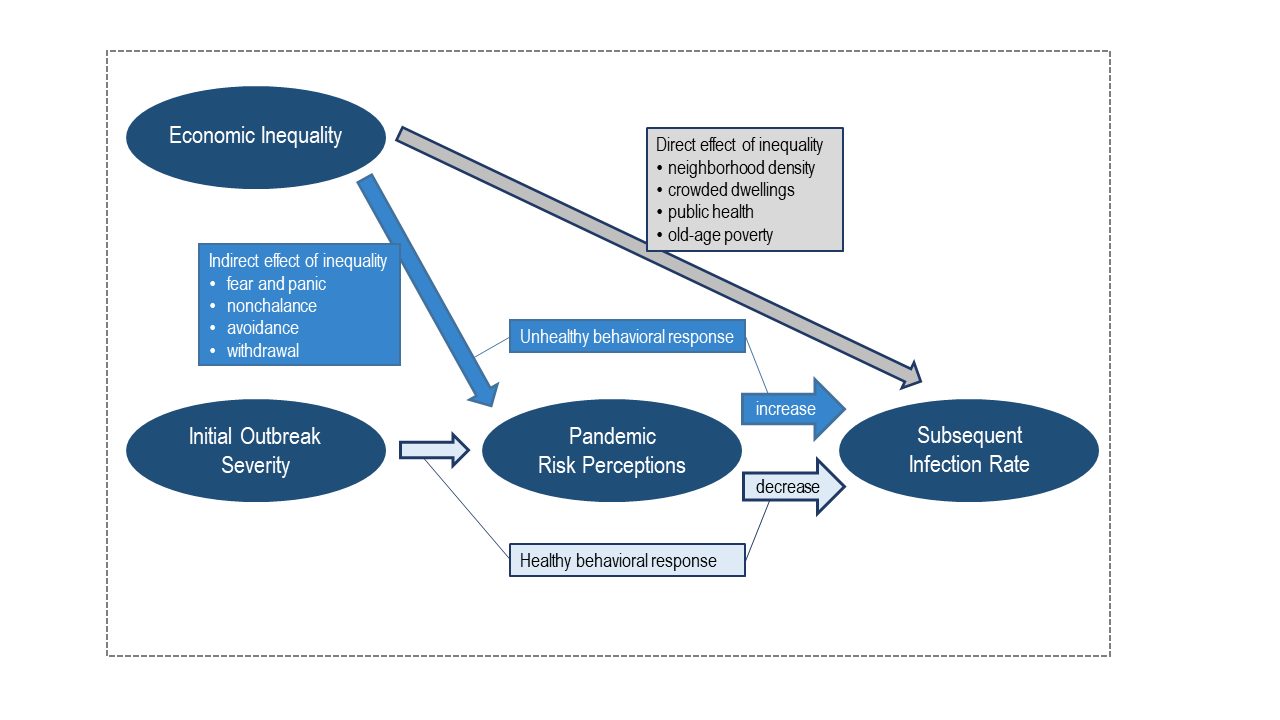
\includegraphics[width=17.78in]{results/Fig1}

\hypertarget{figure-2}{%
\subsection{Figure 2}\label{figure-2}}

As testing rates vary dramatically by country, we measure the number of
deaths with an 18-day lead as a better indicator of the severity of the
outbreak by country. Those who died were inevitably sick or showing
symptoms 18 days prior.

\begin{Shaded}
\begin{Highlighting}[]
\CommentTok{# this means the series ends at 06-01}

\NormalTok{deaths_long <-}\StringTok{ }\KeywordTok{subset}\NormalTok{(deaths_long, date }\OperatorTok{<}\StringTok{ }\KeywordTok{as.Date}\NormalTok{(}\StringTok{"2020-06-02"}\NormalTok{))}

\CommentTok{# keep two extra days for plotting empty space}

\NormalTok{deaths_long}\OperatorTok{$}\NormalTok{dead_lead <-}\StringTok{ }\KeywordTok{ifelse}\NormalTok{(deaths_long}\OperatorTok{$}\NormalTok{date }\OperatorTok{>}\StringTok{ }\KeywordTok{as.Date}\NormalTok{(}\StringTok{"2020-05-31"}\NormalTok{), }\OtherTok{NA}\NormalTok{, deaths_long}\OperatorTok{$}\NormalTok{dead_lead)}

\CommentTok{# Using countries}
\NormalTok{deaths_longC <-}\StringTok{ }\KeywordTok{subset}\NormalTok{(deaths_long, cow }\OperatorTok\StringTok{ }\NormalTok{use_countriesa)}


\CommentTok{# add Country name}
\NormalTok{deaths_longC}\OperatorTok{$}\NormalTok{Country <-}\StringTok{ }\KeywordTok{countrycode}\NormalTok{(deaths_longC}\OperatorTok{$}\NormalTok{cow, }\StringTok{"cown"}\NormalTok{, }\StringTok{"iso3c"}\NormalTok{)}
\NormalTok{deaths_longC}\OperatorTok{$}\NormalTok{Country <-}\StringTok{ }\KeywordTok{ifelse}\NormalTok{(deaths_longC}\OperatorTok{$}\NormalTok{cow }\OperatorTok{==}\StringTok{  }\DecValTok{347}\NormalTok{, }\StringTok{"KOS"}\NormalTok{, deaths_longC}\OperatorTok{$}\NormalTok{Country)}




\CommentTok{# log deaths}
\NormalTok{deaths_longC}\OperatorTok{$}\NormalTok{dead_lead_log <-}\StringTok{ }\KeywordTok{ifelse}\NormalTok{(deaths_longC}\OperatorTok{$}\NormalTok{dead_lead }\OperatorTok{>}\StringTok{ }\DecValTok{3}\NormalTok{,}\KeywordTok{log}\NormalTok{(deaths_longC}\OperatorTok{$}\NormalTok{dead_lead),}\DecValTok{1}\NormalTok{)}

\CommentTok{# squared log deaths to accentuate differences}
\NormalTok{deaths_longC}\OperatorTok{$}\NormalTok{dead_lead_log <-}\StringTok{ }\NormalTok{deaths_longC}\OperatorTok{$}\NormalTok{dead_lead_log}\OperatorTok{*}\NormalTok{deaths_longC}\OperatorTok{$}\NormalTok{dead_lead_log}

\CommentTok{# create a label map so they do not overlap}
\NormalTok{deaths_longCL <-}\StringTok{ }\KeywordTok{subset}\NormalTok{(deaths_longC, date }\OperatorTok{==}\StringTok{ }\KeywordTok{as.Date}\NormalTok{(}\StringTok{"2020-05-31"}\NormalTok{))}
\NormalTok{deaths_longCL <-}\StringTok{ }\NormalTok{deaths_longCL }\OperatorTok
\StringTok{  }\KeywordTok{mutate}\NormalTok{(}\DataTypeTok{date =} \KeywordTok{ifelse}\NormalTok{(Country }\OperatorTok{==}\StringTok{ "DEU"} \OperatorTok{|}\StringTok{ }\NormalTok{Country }\OperatorTok{==}\StringTok{ "RUS"} \OperatorTok{|}\StringTok{ }\NormalTok{Country }\OperatorTok{==}\StringTok{ "TUR"} \OperatorTok{|}\StringTok{ }\NormalTok{Country }\OperatorTok{==}\StringTok{ "ECU"} \OperatorTok{|}\StringTok{ }\NormalTok{Country }\OperatorTok{==}\StringTok{ "COL"} \OperatorTok{|}\StringTok{ }\NormalTok{Country }\OperatorTok{==}\StringTok{ "ZAF"} \OperatorTok{|}\StringTok{ }\NormalTok{Country }\OperatorTok{==}\StringTok{ "PRT"} \OperatorTok{|}\StringTok{ }\NormalTok{Country }\OperatorTok{==}\StringTok{ "BGD"} \OperatorTok{|}\StringTok{ }\NormalTok{Country }\OperatorTok{==}\StringTok{ "CHE"} \OperatorTok{|}\StringTok{ }\NormalTok{Country }\OperatorTok{==}\StringTok{ "UKR"} \OperatorTok{|}\StringTok{ }\NormalTok{Country }\OperatorTok{==}\StringTok{ "JPN"} \OperatorTok{|}\StringTok{ }\NormalTok{Country }\OperatorTok{==}\StringTok{ "DNK"} \OperatorTok{|}\StringTok{ }\NormalTok{Country }\OperatorTok{==}\StringTok{ "AFG"} \OperatorTok{|}\StringTok{ }\NormalTok{Country }\OperatorTok{==}\StringTok{ "CZE"} \OperatorTok{|}\StringTok{ }\NormalTok{Country }\OperatorTok{==}\StringTok{ "ISR"} \OperatorTok{|}\StringTok{ }\NormalTok{Country }\OperatorTok{==}\StringTok{ "KOR"} \OperatorTok{|}\StringTok{ }\NormalTok{Country }\OperatorTok{==}\StringTok{ "MAR"} \OperatorTok{|}\StringTok{ }\NormalTok{Country }\OperatorTok{==}\StringTok{ "GRC"} \OperatorTok{|}\StringTok{ }\NormalTok{Country }\OperatorTok{==}\StringTok{ "LUX"} \OperatorTok{|}\StringTok{ }\NormalTok{Country }\OperatorTok{==}\StringTok{ "HRV"} \OperatorTok{|}\StringTok{ }\NormalTok{Country }\OperatorTok{==}\StringTok{ "LTU"} \OperatorTok{|}\StringTok{ }\NormalTok{Country }\OperatorTok{==}\StringTok{ "ALB"} \OperatorTok{|}\StringTok{ }\NormalTok{Country }\OperatorTok{==}\StringTok{ "KGZ"} \OperatorTok{|}\StringTok{ }\NormalTok{Country }\OperatorTok{==}\StringTok{ "SVK"} \OperatorTok{|}\StringTok{ }\NormalTok{Country }\OperatorTok{==}\StringTok{ "NZL"} \OperatorTok{|}\StringTok{ }\NormalTok{Country }\OperatorTok{==}\StringTok{ "GEO"} \OperatorTok{|}\StringTok{ }\NormalTok{Country }\OperatorTok{==}\StringTok{ "ISL"} \OperatorTok{|}\StringTok{ }\NormalTok{Country }\OperatorTok{==}\StringTok{ "VNM"} \OperatorTok{|}\StringTok{ }\NormalTok{Country }\OperatorTok{==}\StringTok{ "TWN"}\NormalTok{, }\StringTok{"2020-06-06"}\NormalTok{, }\StringTok{"2020-06-01"}\NormalTok{),}
         \DataTypeTok{dead_lead_log =} \KeywordTok{ifelse}\NormalTok{(Country }\OperatorTok{==}\StringTok{ "CHE"}\NormalTok{, }\FloatTok{59.1}\NormalTok{, dead_lead_log),}
         \DataTypeTok{dead_lead_log =} \KeywordTok{ifelse}\NormalTok{(Country }\OperatorTok{==}\StringTok{ "DNK"}\NormalTok{, }\FloatTok{41.8}\NormalTok{, dead_lead_log),}
         \DataTypeTok{dead_lead_log =} \KeywordTok{ifelse}\NormalTok{(Country }\OperatorTok{==}\StringTok{ "UKR"}\NormalTok{, }\FloatTok{48.8}\NormalTok{, dead_lead_log),}
         \DataTypeTok{dead_lead_log =} \KeywordTok{ifelse}\NormalTok{(Country }\OperatorTok{==}\StringTok{ "CZE"}\NormalTok{, }\FloatTok{34.5}\NormalTok{, dead_lead_log),}
         \DataTypeTok{dead_lead_log =} \KeywordTok{ifelse}\NormalTok{(Country }\OperatorTok{==}\StringTok{ "KOR"}\NormalTok{, }\FloatTok{30.6}\NormalTok{, dead_lead_log),}
         \DataTypeTok{dead_lead_log =} \KeywordTok{ifelse}\NormalTok{(Country }\OperatorTok{==}\StringTok{ "MYS"}\NormalTok{, }\FloatTok{24.2}\NormalTok{, dead_lead_log),}
         \DataTypeTok{dead_lead_log =} \KeywordTok{ifelse}\NormalTok{(Country }\OperatorTok{==}\StringTok{ "AUS"}\NormalTok{, }\FloatTok{21.8}\NormalTok{, dead_lead_log),}
         \DataTypeTok{dead_lead_log =} \KeywordTok{ifelse}\NormalTok{(Country }\OperatorTok{==}\StringTok{ "LUX"}\NormalTok{, }\FloatTok{23.8}\NormalTok{, dead_lead_log),}
         \DataTypeTok{dead_lead_log =} \KeywordTok{ifelse}\NormalTok{(Country }\OperatorTok{==}\StringTok{ "FIN"}\NormalTok{, }\FloatTok{34.5}\NormalTok{, dead_lead_log),}
         \DataTypeTok{dead_lead_log =} \KeywordTok{ifelse}\NormalTok{(Country }\OperatorTok{==}\StringTok{ "KOS"}\NormalTok{, }\DecValTok{14}\NormalTok{, dead_lead_log),}
         \DataTypeTok{dead_lead_log =} \KeywordTok{ifelse}\NormalTok{(Country }\OperatorTok{==}\StringTok{ "ALB"}\NormalTok{, }\FloatTok{14.5}\NormalTok{, dead_lead_log),}
         \DataTypeTok{dead_lead_log =} \KeywordTok{ifelse}\NormalTok{(Country }\OperatorTok{==}\StringTok{ "LVA"}\NormalTok{, }\FloatTok{12.5}\NormalTok{, dead_lead_log),}
         \DataTypeTok{dead_lead_log =} \KeywordTok{ifelse}\NormalTok{(Country }\OperatorTok{==}\StringTok{ "GRC"}\NormalTok{, }\FloatTok{26.8}\NormalTok{, dead_lead_log),}
         \DataTypeTok{dead_lead_log =} \KeywordTok{ifelse}\NormalTok{(Country }\OperatorTok{==}\StringTok{ "KGZ"}\NormalTok{, }\FloatTok{12.5}\NormalTok{, dead_lead_log),}
         \DataTypeTok{dead_lead_log =} \KeywordTok{ifelse}\NormalTok{(Country }\OperatorTok{==}\StringTok{ "NZL"}\NormalTok{, }\DecValTok{9}\NormalTok{, dead_lead_log),}
         \DataTypeTok{dead_lead_log =} \KeywordTok{ifelse}\NormalTok{(Country }\OperatorTok{==}\StringTok{ "SVK"}\NormalTok{, }\FloatTok{10.5}\NormalTok{, dead_lead_log),}
         \DataTypeTok{dead_lead_log =} \KeywordTok{ifelse}\NormalTok{(Country }\OperatorTok{==}\StringTok{ "MEX"}\NormalTok{, }\DecValTok{99}\NormalTok{, dead_lead_log),}
         \DataTypeTok{dead_lead_log =} \KeywordTok{ifelse}\NormalTok{(Country }\OperatorTok{==}\StringTok{ "ESP"}\NormalTok{, }\FloatTok{103.8}\NormalTok{, dead_lead_log),}
         \DataTypeTok{dead_lead_log =} \KeywordTok{ifelse}\NormalTok{(Country }\OperatorTok{==}\StringTok{ "CRI"}\NormalTok{, }\FloatTok{7.35}\NormalTok{, dead_lead_log),}
         \DataTypeTok{dead_lead_log =} \KeywordTok{ifelse}\NormalTok{(Country }\OperatorTok{==}\StringTok{ "SLV"}\NormalTok{, }\FloatTok{5.78}\NormalTok{, dead_lead_log),}
         \DataTypeTok{dead_lead_log =} \KeywordTok{ifelse}\NormalTok{(Country }\OperatorTok{==}\StringTok{ "BRN"}\NormalTok{, }\FloatTok{2.6}\NormalTok{, dead_lead_log),}
         \DataTypeTok{dead_lead_log =} \KeywordTok{ifelse}\NormalTok{(Country }\OperatorTok{==}\StringTok{ "TWN"}\NormalTok{, }\DecValTok{3}\NormalTok{, dead_lead_log),}
         \DataTypeTok{dead_lead_log =} \KeywordTok{ifelse}\NormalTok{(Country }\OperatorTok{==}\StringTok{ "MLT"}\NormalTok{, }\FloatTok{4.16}\NormalTok{, dead_lead_log),}
         \DataTypeTok{dead_lead_log =} \KeywordTok{ifelse}\NormalTok{(Country }\OperatorTok{==}\StringTok{ "SWE"}\NormalTok{, }\FloatTok{73.2}\NormalTok{, dead_lead_log),}
         \DataTypeTok{dead_lead_log =} \KeywordTok{ifelse}\NormalTok{(Country }\OperatorTok{==}\StringTok{ "ZAF"}\NormalTok{, }\FloatTok{55.5}\NormalTok{, dead_lead_log),}
          \DataTypeTok{dead_lead_log =} \KeywordTok{ifelse}\NormalTok{(Country }\OperatorTok{==}\StringTok{ "ROU"}\NormalTok{, }\FloatTok{53.4}\NormalTok{, dead_lead_log),}
         \DataTypeTok{dead_lead_log =} \KeywordTok{ifelse}\NormalTok{(Country }\OperatorTok{==}\StringTok{ "ISL"}\NormalTok{, }\FloatTok{5.15}\NormalTok{, dead_lead_log),}
         \DataTypeTok{dead_lead_log =} \KeywordTok{ifelse}\NormalTok{(Country }\OperatorTok{==}\StringTok{ "CYP"}\NormalTok{, }\FloatTok{8.95}\NormalTok{, dead_lead_log),}
         \DataTypeTok{dead_lead_log =} \KeywordTok{ifelse}\NormalTok{(Country }\OperatorTok{==}\StringTok{ "SVK"}\NormalTok{, }\FloatTok{10.8}\NormalTok{, dead_lead_log))}

\CommentTok{# second go at labels}
\NormalTok{deaths_longCLa <-}\StringTok{ }\NormalTok{deaths_longCL}


\CommentTok{# labels need adjustment}
\NormalTok{deaths_longCLa <-}\StringTok{ }\NormalTok{deaths_longCLa }\OperatorTok
\StringTok{  }\KeywordTok{mutate}\NormalTok{(}\DataTypeTok{dead_lead_log =} \KeywordTok{ifelse}\NormalTok{(Country }\OperatorTok{==}\StringTok{ "AUS"}\NormalTok{, }\FloatTok{20.2}\NormalTok{, dead_lead_log),}
         \DataTypeTok{dead_lead_log =} \KeywordTok{ifelse}\NormalTok{(Country }\OperatorTok{==}\StringTok{ "BIH"}\NormalTok{, }\FloatTok{25.3}\NormalTok{, dead_lead_log),}
         \DataTypeTok{dead_lead_log =} \KeywordTok{ifelse}\NormalTok{(Country }\OperatorTok{==}\StringTok{ "BGR"}\NormalTok{, }\FloatTok{26.9}\NormalTok{, dead_lead_log),}
         \DataTypeTok{dead_lead_log =} \KeywordTok{ifelse}\NormalTok{(Country }\OperatorTok{==}\StringTok{ "MKD"}\NormalTok{, }\FloatTok{28.6}\NormalTok{, dead_lead_log),}
         \DataTypeTok{dead_lead_log =} \KeywordTok{ifelse}\NormalTok{(Country }\OperatorTok{==}\StringTok{ "MYS"}\NormalTok{, }\FloatTok{23.6}\NormalTok{, dead_lead_log))}


\NormalTok{fig2 <-}\StringTok{ }\KeywordTok{ggplot}\NormalTok{(}\DataTypeTok{data=}\NormalTok{deaths_longC, }\KeywordTok{aes}\NormalTok{(}\DataTypeTok{x=}\NormalTok{date , }\DataTypeTok{y=}\NormalTok{dead_lead_log, }\DataTypeTok{group=}\NormalTok{Country, }\DataTypeTok{color=}\NormalTok{Country)) }\OperatorTok{+}
\StringTok{    }\KeywordTok{geom_line}\NormalTok{() }\OperatorTok{+}
\StringTok{  }\KeywordTok{labs}\NormalTok{(}\DataTypeTok{x=} \StringTok{""}\NormalTok{, }\DataTypeTok{y =} \StringTok{"Outbreak Severity (18 day lead of COVID-19 deaths)"}\NormalTok{) }\OperatorTok{+}
\StringTok{  }\KeywordTok{geom_segment}\NormalTok{(}\KeywordTok{aes}\NormalTok{(}\DataTypeTok{x =} \KeywordTok{as.Date}\NormalTok{(}\StringTok{"2020-03-27"}\NormalTok{), }\DataTypeTok{y =} \DecValTok{1}\NormalTok{, }\DataTypeTok{xend =} \KeywordTok{as.Date}\NormalTok{(}\StringTok{"2020-03-27"}\NormalTok{), }\DataTypeTok{yend =} \DecValTok{135}\NormalTok{), }\DataTypeTok{linetype =} \StringTok{"dashed"}\NormalTok{, }\DataTypeTok{color =} \StringTok{"black"}\NormalTok{, }\DataTypeTok{size =} \FloatTok{0.8}\NormalTok{) }\OperatorTok{+}
\StringTok{  }\KeywordTok{geom_segment}\NormalTok{(}\KeywordTok{aes}\NormalTok{(}\DataTypeTok{x =} \KeywordTok{as.Date}\NormalTok{(}\StringTok{"2020-04-30"}\NormalTok{), }\DataTypeTok{y =} \DecValTok{1}\NormalTok{, }\DataTypeTok{xend =} \KeywordTok{as.Date}\NormalTok{(}\StringTok{"2020-04-30"}\NormalTok{), }\DataTypeTok{yend =} \DecValTok{135}\NormalTok{), }\DataTypeTok{linetype =} \StringTok{"dashed"}\NormalTok{, }\DataTypeTok{color =} \StringTok{"black"}\NormalTok{, }\DataTypeTok{size =} \FloatTok{0.8}\NormalTok{) }\OperatorTok{+}
\StringTok{  }\KeywordTok{annotate}\NormalTok{(}\StringTok{"text"}\NormalTok{, }\DataTypeTok{x=} \KeywordTok{as.Date}\NormalTok{(}\StringTok{"2020-01-21"}\NormalTok{), }\DataTypeTok{y=} \DecValTok{5}\NormalTok{, }
           \DataTypeTok{label=}\StringTok{"5"}\NormalTok{, }\DataTypeTok{size=}\FloatTok{4.5}\NormalTok{, }\DataTypeTok{color =} \StringTok{"gray20"}\NormalTok{) }\OperatorTok{+}
\StringTok{  }\KeywordTok{annotate}\NormalTok{(}\StringTok{"text"}\NormalTok{, }\DataTypeTok{x=} \KeywordTok{as.Date}\NormalTok{(}\StringTok{"2020-01-21"}\NormalTok{), }\DataTypeTok{y=} \DecValTok{30}\NormalTok{, }
           \DataTypeTok{label=}\StringTok{"250"}\NormalTok{, }\DataTypeTok{size=}\FloatTok{4.5}\NormalTok{, }\DataTypeTok{color =} \StringTok{"gray20"}\NormalTok{) }\OperatorTok{+}
\StringTok{  }\KeywordTok{annotate}\NormalTok{(}\StringTok{"text"}\NormalTok{, }\DataTypeTok{x=} \KeywordTok{as.Date}\NormalTok{(}\StringTok{"2020-01-21"}\NormalTok{), }\DataTypeTok{y=} \DecValTok{55}\NormalTok{, }
           \DataTypeTok{label=}\StringTok{"2k"}\NormalTok{, }\DataTypeTok{size=}\FloatTok{4.5}\NormalTok{, }\DataTypeTok{color =} \StringTok{"gray20"}\NormalTok{) }\OperatorTok{+}
\StringTok{  }\KeywordTok{annotate}\NormalTok{(}\StringTok{"text"}\NormalTok{, }\DataTypeTok{x=} \KeywordTok{as.Date}\NormalTok{(}\StringTok{"2020-01-21"}\NormalTok{), }\DataTypeTok{y=} \DecValTok{80}\NormalTok{, }
           \DataTypeTok{label=}\StringTok{"8k"}\NormalTok{, }\DataTypeTok{size=}\FloatTok{4.5}\NormalTok{, }\DataTypeTok{color =} \StringTok{"gray20"}\NormalTok{) }\OperatorTok{+}
\StringTok{  }\KeywordTok{annotate}\NormalTok{(}\StringTok{"text"}\NormalTok{, }\DataTypeTok{x=} \KeywordTok{as.Date}\NormalTok{(}\StringTok{"2020-01-21"}\NormalTok{), }\DataTypeTok{y=} \DecValTok{105}\NormalTok{, }
           \DataTypeTok{label=}\StringTok{"30k"}\NormalTok{, }\DataTypeTok{size=}\FloatTok{4.5}\NormalTok{, }\DataTypeTok{color =} \StringTok{"gray20"}\NormalTok{) }\OperatorTok{+}
\StringTok{  }\KeywordTok{annotate}\NormalTok{(}\StringTok{"text"}\NormalTok{, }\DataTypeTok{x=} \KeywordTok{as.Date}\NormalTok{(}\StringTok{"2020-01-21"}\NormalTok{), }\DataTypeTok{y=} \DecValTok{130}\NormalTok{, }
           \DataTypeTok{label=}\StringTok{"120k"}\NormalTok{, }\DataTypeTok{size=}\FloatTok{4.5}\NormalTok{, }\DataTypeTok{color =} \StringTok{"gray20"}\NormalTok{) }\OperatorTok{+}
\StringTok{  }\KeywordTok{annotate}\NormalTok{(}\StringTok{"text"}\NormalTok{, }\DataTypeTok{x=} \KeywordTok{as.Date}\NormalTok{(}\StringTok{"2020-04-13"}\NormalTok{), }\DataTypeTok{y=}\DecValTok{137}\NormalTok{, }\DataTypeTok{label=}\StringTok{"survey time-frame"}\NormalTok{, }\DataTypeTok{size =} \DecValTok{4}\NormalTok{, }\DataTypeTok{color=}\StringTok{"black"}\NormalTok{) }\OperatorTok{+}
\StringTok{  }\KeywordTok{scale_x_date}\NormalTok{(}\DataTypeTok{date_breaks =} \StringTok{"2 weeks"}\NormalTok{ , }\DataTypeTok{date_labels =} \StringTok{"%d-%b"}\NormalTok{) }\OperatorTok{+}
\StringTok{  }\KeywordTok{geom_text}\NormalTok{(}\DataTypeTok{data =}\NormalTok{ deaths_longCLa, }\KeywordTok{aes}\NormalTok{(}\DataTypeTok{label =}\NormalTok{ Country, }\DataTypeTok{colour =}\NormalTok{ Country, }\DataTypeTok{x =} \KeywordTok{as.Date}\NormalTok{(date), }\DataTypeTok{y =}\NormalTok{ dead_lead_log, }\DataTypeTok{hjust =} \FloatTok{-.1}\NormalTok{), }\DataTypeTok{size =} \FloatTok{2.62}\NormalTok{) }\OperatorTok{+}
\StringTok{  }\KeywordTok{theme}\NormalTok{(}\DataTypeTok{legend.position =} \StringTok{"none"}\NormalTok{,}
        \DataTypeTok{panel.background =} \KeywordTok{element_blank}\NormalTok{(),}
        \DataTypeTok{axis.text.y =} \KeywordTok{element_blank}\NormalTok{(),}
        \DataTypeTok{axis.ticks =} \KeywordTok{element_blank}\NormalTok{(),}
        \DataTypeTok{axis.title.y =} \KeywordTok{element_text}\NormalTok{(}\DataTypeTok{size=}\DecValTok{14}\NormalTok{, }\DataTypeTok{vjust=}\OperatorTok{-}\FloatTok{0.5}\NormalTok{),}
        \DataTypeTok{axis.text.x =} \KeywordTok{element_text}\NormalTok{(}\DataTypeTok{vjust=}\DecValTok{1}\NormalTok{, }\DataTypeTok{hjust=}\FloatTok{0.35}\NormalTok{, }\DataTypeTok{color =} \StringTok{"gray20"}\NormalTok{, }\DataTypeTok{size =} \DecValTok{12}\NormalTok{),}
        \DataTypeTok{plot.margin =} \KeywordTok{margin}\NormalTok{(}\DecValTok{0}\NormalTok{, }\DecValTok{1}\NormalTok{, }\DecValTok{0}\NormalTok{, }\DecValTok{0}\NormalTok{, }\StringTok{"cm"}\NormalTok{))}

\CommentTok{# log conversion}
\CommentTok{# 30 = 250}
\CommentTok{# 55 = 2,000}
\CommentTok{# 80 = 8,000}
\CommentTok{# 105 = 28,000}
\CommentTok{# 130 = 120,000}
\KeywordTok{agg_png}\NormalTok{(}\DataTypeTok{file =} \StringTok{"results/Fig2.png"}\NormalTok{, }\DataTypeTok{width =} \DecValTok{1200}\NormalTok{, }\DataTypeTok{height =} \DecValTok{1020}\NormalTok{,  }\DataTypeTok{res =} \DecValTok{144}\NormalTok{)}
\KeywordTok{print}\NormalTok{(fig2)}
\KeywordTok{dev.off}\NormalTok{()}
\end{Highlighting}
\end{Shaded}

\begin{verbatim}
## pdf 
##   2
\end{verbatim}

\begin{Shaded}
\begin{Highlighting}[]
\NormalTok{knitr}\OperatorTok{::}\KeywordTok{include_graphics}\NormalTok{(}\StringTok{"results/Fig2.png"}\NormalTok{)}
\end{Highlighting}
\end{Shaded}

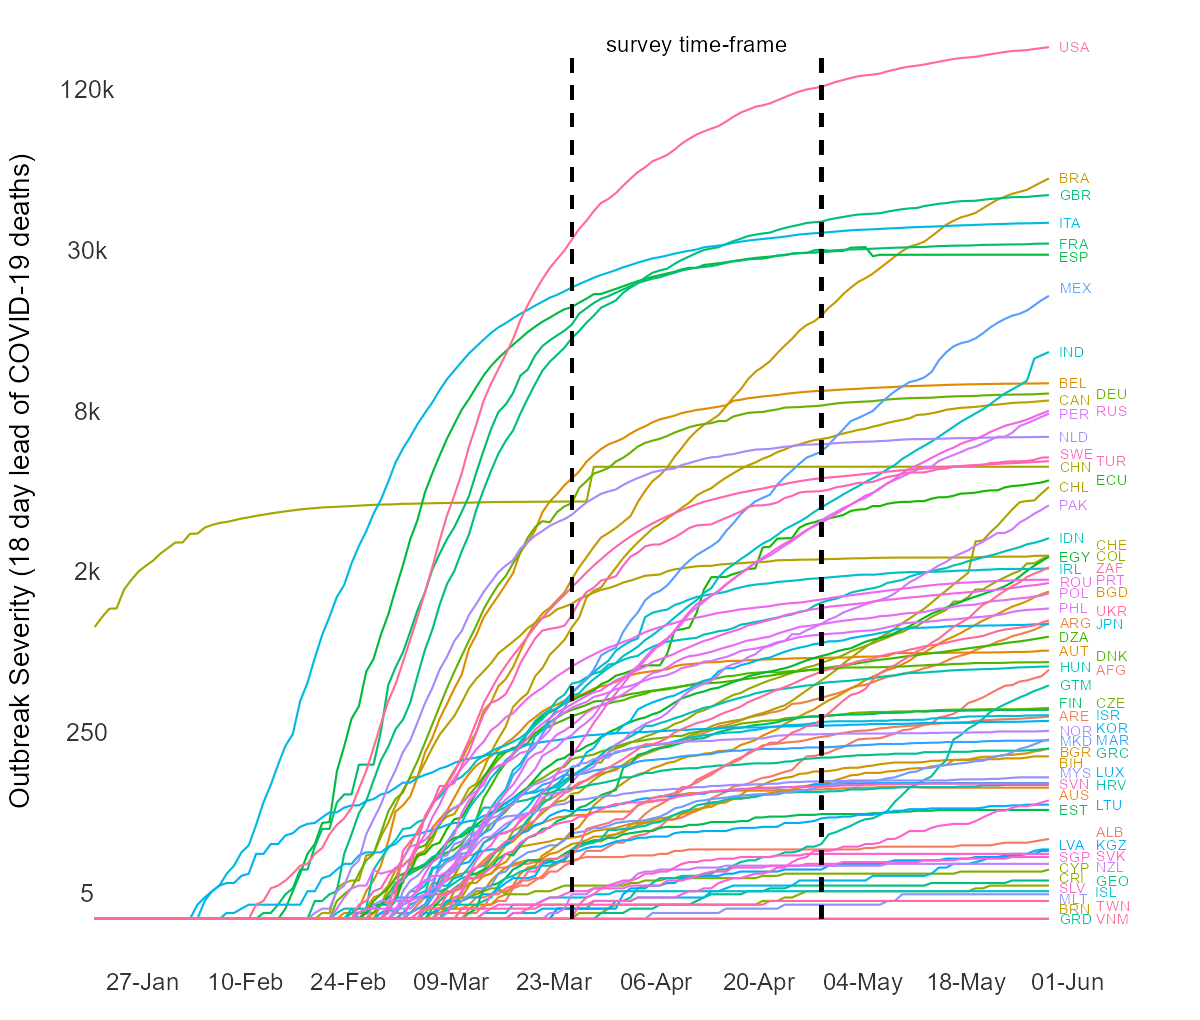
\includegraphics[width=16.67in]{results/Fig2}

\begin{Shaded}
\begin{Highlighting}[]
\KeywordTok{rm}\NormalTok{(deaths_longCL, deaths_longCLa)}
\end{Highlighting}
\end{Shaded}

\hypertarget{final-data-adjustments}{%
\subsection{Final Data Adjustments}\label{final-data-adjustments}}

\hypertarget{set-up-18-day-lead}{%
\paragraph{Set up 18-Day lead}\label{set-up-18-day-lead}}

\begin{Shaded}
\begin{Highlighting}[]
\NormalTok{infect_merge <-}\StringTok{ }\KeywordTok{as.data.frame}\NormalTok{(}\KeywordTok{matrix}\NormalTok{(}\DataTypeTok{nrow =} \DecValTok{74}\NormalTok{, }\DataTypeTok{ncol =} \DecValTok{1}\NormalTok{))}
\NormalTok{infect_merge[}\DecValTok{1}\OperatorTok{:}\DecValTok{74}\NormalTok{,}\DecValTok{1}\NormalTok{] <-}\StringTok{ }\KeywordTok{as.numeric}\NormalTok{(use_countriesa)}
\KeywordTok{colnames}\NormalTok{(infect_merge) <-}\StringTok{ }\KeywordTok{c}\NormalTok{(}\StringTok{"cow"}\NormalTok{)}

\NormalTok{d1 <-}\StringTok{ }\KeywordTok{subset}\NormalTok{(deaths_longC, date }\OperatorTok{==}\StringTok{ "2020-05-01"}\NormalTok{, }\DataTypeTok{select =} \KeywordTok{c}\NormalTok{(cow, dead_lead))}
\NormalTok{d2 <-}\StringTok{ }\KeywordTok{subset}\NormalTok{(deaths_longC, date }\OperatorTok{==}\StringTok{ "2020-05-31"}\NormalTok{, }\DataTypeTok{select =} \KeywordTok{c}\NormalTok{(cow, dead_lead, dead_1st_date))}

\NormalTok{infect_merge <-}\StringTok{ }\KeywordTok{left_join}\NormalTok{(infect_merge, d1, }\DataTypeTok{by =} \StringTok{"cow"}\NormalTok{)}
\NormalTok{infect_merge <-}\StringTok{ }\KeywordTok{left_join}\NormalTok{(infect_merge, d2, }\DataTypeTok{by =} \StringTok{"cow"}\NormalTok{)}

\KeywordTok{colnames}\NormalTok{(infect_merge) <-}\StringTok{ }\KeywordTok{c}\NormalTok{(}\StringTok{"cow"}\NormalTok{,}\StringTok{"dead_lead_may1"}\NormalTok{,}\StringTok{"dead_lead_may31"}\NormalTok{,}\StringTok{"dead_1st_date"}\NormalTok{)}

\KeywordTok{rm}\NormalTok{(d1,d2)}

\NormalTok{df <-}\StringTok{ }\KeywordTok{left_join}\NormalTok{(finaldf_C, infect_merge, }\DataTypeTok{by =} \StringTok{"cow"}\NormalTok{)}

\CommentTok{# fix Argentina and Indonesia (last top1 observation was 2004)}
\NormalTok{df}\OperatorTok{$}\NormalTok{top1 <-}\StringTok{ }\KeywordTok{ifelse}\NormalTok{(df}\OperatorTok{$}\NormalTok{cow }\OperatorTok{==}\StringTok{ }\DecValTok{160}\NormalTok{, }\FloatTok{.168}\NormalTok{, }\KeywordTok{ifelse}\NormalTok{(df}\OperatorTok{$}\NormalTok{cow }\OperatorTok{==}\StringTok{ }\DecValTok{850}\NormalTok{, }\FloatTok{.085}\NormalTok{, df}\OperatorTok{$}\NormalTok{top1))}
\end{Highlighting}
\end{Shaded}

\hypertarget{infection-increase-ratio-may-1-31}{%
\paragraph{Infection Increase (Ratio May
1-31)}\label{infection-increase-ratio-may-1-31}}

\begin{Shaded}
\begin{Highlighting}[]
\CommentTok{# There was a change in reporting in Spain and the deaths dropped suddenly on May 6th, adjust for this here. }

\NormalTok{df}\OperatorTok{$}\NormalTok{dead_lead_may1 <-}\StringTok{ }\KeywordTok{ifelse}\NormalTok{(df}\OperatorTok{$}\NormalTok{cow }\OperatorTok{==}\StringTok{ }\DecValTok{230}\NormalTok{, }\DecValTok{27000}\NormalTok{, df}\OperatorTok{$}\NormalTok{dead_lead_may1)}
\NormalTok{df <-}\StringTok{ }\NormalTok{df }\OperatorTok
\StringTok{  }\KeywordTok{mutate}\NormalTok{(}\DataTypeTok{rate_2 =} \KeywordTok{ifelse}\NormalTok{(dead_lead_may31 }\OperatorTok{==}\StringTok{ }\DecValTok{0}\NormalTok{, }\DecValTok{0}\NormalTok{, (dead_lead_may31 }\OperatorTok{-}\StringTok{ }\NormalTok{dead_lead_may1) }\OperatorTok{/}\StringTok{ }\NormalTok{(dead_lead_may1)),}
         \DataTypeTok{rate_2 =} \KeywordTok{ifelse}\NormalTok{(rate_}\DecValTok{2} \OperatorTok{>}\StringTok{ }\DecValTok{3}\NormalTok{, }\DecValTok{3}\NormalTok{, rate_}\DecValTok{2}\NormalTok{) }\CommentTok{# trim outliers}
\NormalTok{  )}

\CommentTok{# deaths per capita May 1-31}
\NormalTok{df}\OperatorTok{$}\NormalTok{newdthpc <-}\StringTok{ }\NormalTok{(df}\OperatorTok{$}\NormalTok{dead_lead_may31 }\OperatorTok{-}\StringTok{ }\NormalTok{df}\OperatorTok{$}\NormalTok{dead_lead_may1)}\OperatorTok{/}\NormalTok{df}\OperatorTok{$}\NormalTok{pop}
\CommentTok{#make per 10,000 instead of per 1,000}
\NormalTok{df}\OperatorTok{$}\NormalTok{newdthpc10 <-}\StringTok{ }\NormalTok{df}\OperatorTok{$}\NormalTok{newdthpc}\OperatorTok{*}\DecValTok{10}
\NormalTok{df}\OperatorTok{$}\NormalTok{rate_}\DecValTok{3}\NormalTok{ <-}\StringTok{ }\NormalTok{df}\OperatorTok{$}\NormalTok{newdthpc10}
\end{Highlighting}
\end{Shaded}

\hypertarget{squared-terms}{%
\paragraph{Squared Terms}\label{squared-terms}}

\begin{Shaded}
\begin{Highlighting}[]
\NormalTok{df <-}\StringTok{ }\NormalTok{df }\OperatorTok
\StringTok{  }\KeywordTok{mutate}\NormalTok{(}\DataTypeTok{gini_dispR =}\NormalTok{ gini_disp}\OperatorTok{/}\DecValTok{100}\NormalTok{, }\CommentTok{# make gini smaller to keep boundaries reasonable in SEM}
         \DataTypeTok{gini_disp2 =}\NormalTok{ gini_dispR}\OperatorTok{^}\DecValTok{2}\NormalTok{,}
         \DataTypeTok{concern_self2 =}\NormalTok{ concern_self}\OperatorTok{^}\DecValTok{2}\NormalTok{,}
         \DataTypeTok{gini_disp2C =}\NormalTok{ gini_disp2 }\OperatorTok{-}\StringTok{ }\KeywordTok{mean}\NormalTok{(gini_disp2),}
         \DataTypeTok{concern_self2C =}\NormalTok{ concern_self2 }\OperatorTok{-}\StringTok{ }\KeywordTok{mean}\NormalTok{(concern_self2))}
\end{Highlighting}
\end{Shaded}

\hypertarget{main-models}{%
\subsection{Main Models}\label{main-models}}

\hypertarget{statistics}{%
\subsubsection{Statistics}\label{statistics}}

\hypertarget{set-up-first-models-baseline-models}{%
\paragraph{Set up first models (baseline
models)}\label{set-up-first-models-baseline-models}}

M1 Timing + severity of outbreak should predict risk perceptions. M22
Risk perceptions + risk perceptions-curve should predict deaths.

\begin{Shaded}
\begin{Highlighting}[]
\CommentTok{# adjust risk for severity of outbreak}
\NormalTok{m1 <-}\StringTok{ }\KeywordTok{lm}\NormalTok{(concern_self }\OperatorTok{~}\StringTok{ }\NormalTok{days_since_peak }\OperatorTok{+}\StringTok{ }\NormalTok{conf_delta }\OperatorTok{+}\StringTok{ }\NormalTok{gov_resp, }\DataTypeTok{data =}\NormalTok{ df)}

\CommentTok{# predicted values}
\NormalTok{df}\OperatorTok{$}\NormalTok{m1p <-}\StringTok{ }\KeywordTok{predict.lm}\NormalTok{(m1, df)}

\CommentTok{# residuals}
\NormalTok{df}\OperatorTok{$}\NormalTok{m1r <-}\StringTok{ }\NormalTok{df}\OperatorTok{$}\NormalTok{concern_self }\OperatorTok{-}\StringTok{ }\NormalTok{df}\OperatorTok{$}\NormalTok{m1p }

\NormalTok{m1a <-}\StringTok{ }\KeywordTok{summary}\NormalTok{(m1)}
\NormalTok{m1a <-}\StringTok{ }\KeywordTok{paste0}\NormalTok{(}\StringTok{"Adjusted r-square = "}\NormalTok{, }\KeywordTok{round}\NormalTok{(m1a[[}\StringTok{"r.squared"}\NormalTok{]],}\DecValTok{3}\NormalTok{))}

\NormalTok{m23 <-}\StringTok{ }\KeywordTok{lm}\NormalTok{(rate_}\DecValTok{2} \OperatorTok{~}\StringTok{ }\NormalTok{days_since_peak }\OperatorTok{+}\StringTok{ }\NormalTok{conf_delta }\OperatorTok{+}\StringTok{ }\NormalTok{gov_resp }\OperatorTok{+}\StringTok{ }\NormalTok{concern_self }\OperatorTok{+}\StringTok{ }\KeywordTok{I}\NormalTok{(concern_self}\OperatorTok{^}\DecValTok{2}\NormalTok{), }\DataTypeTok{data =}\NormalTok{ df)}
\end{Highlighting}
\end{Shaded}

\hypertarget{descriptives}{%
\paragraph{Descriptives}\label{descriptives}}

\begin{Shaded}
\begin{Highlighting}[]
\NormalTok{cor <-}\StringTok{ }\KeywordTok{select}\NormalTok{(df, concern_self, concern_self_se, days_since_peak, conf_delta, gov_resp, rate_}\DecValTok{2}\NormalTok{, rate_}\DecValTok{3}\NormalTok{, gini_disp, top1, socpolicy, gdp)}

\NormalTok{corm <-}\StringTok{ }\NormalTok{cor }\OperatorTok
\StringTok{  }\KeywordTok{mutate}\NormalTok{(}\DataTypeTok{concern_selfsd =} \KeywordTok{sd}\NormalTok{(concern_self, }\DataTypeTok{na.rm =}\NormalTok{ T),}
         \DataTypeTok{concern_self_sesd =} \KeywordTok{sd}\NormalTok{(concern_self_se, }\DataTypeTok{na.rm =}\NormalTok{ T),}
         \DataTypeTok{days_since_peaksd =} \KeywordTok{sd}\NormalTok{(days_since_peak, }\DataTypeTok{na.rm =}\NormalTok{ T),}
         \DataTypeTok{conf_deltasd =} \KeywordTok{sd}\NormalTok{(conf_delta, }\DataTypeTok{na.rm =}\NormalTok{ T),}
         \DataTypeTok{gov_respsd =} \KeywordTok{sd}\NormalTok{(gov_resp, }\DataTypeTok{na.rm =}\NormalTok{ T),}
         \DataTypeTok{rate_2sd =} \KeywordTok{sd}\NormalTok{(rate_}\DecValTok{2}\NormalTok{, }\DataTypeTok{na.rm =}\NormalTok{ T),}
         \DataTypeTok{rate_3sd =} \KeywordTok{sd}\NormalTok{(rate_}\DecValTok{3}\NormalTok{, }\DataTypeTok{na.rm =}\NormalTok{ T),}
         \DataTypeTok{gini_dispsd =} \KeywordTok{sd}\NormalTok{(gini_disp, }\DataTypeTok{na.rm =}\NormalTok{ T),}
         \DataTypeTok{top1sd =} \KeywordTok{sd}\NormalTok{(top1, }\DataTypeTok{na.rm =}\NormalTok{ T),}
         \DataTypeTok{socpolicysd =} \KeywordTok{sd}\NormalTok{(socpolicy, }\DataTypeTok{na.rm =}\NormalTok{ T),}
         \DataTypeTok{gdpsd =} \KeywordTok{sd}\NormalTok{(gdp, }\DataTypeTok{na.rm =}\NormalTok{ T),}\DataTypeTok{concern_self_min =} \KeywordTok{min}\NormalTok{(concern_self, }\DataTypeTok{na.rm =}\NormalTok{ T),}
         \DataTypeTok{concern_self_se_min =} \KeywordTok{min}\NormalTok{(concern_self_se, }\DataTypeTok{na.rm =}\NormalTok{ T),}
         \DataTypeTok{days_since_peak_min =} \KeywordTok{min}\NormalTok{(days_since_peak, }\DataTypeTok{na.rm =}\NormalTok{ T),}
         \DataTypeTok{conf_delta_min =} \KeywordTok{min}\NormalTok{(conf_delta, }\DataTypeTok{na.rm =}\NormalTok{ T),}
         \DataTypeTok{gov_resp_min =} \KeywordTok{min}\NormalTok{(gov_resp, }\DataTypeTok{na.rm =}\NormalTok{ T),}
         \DataTypeTok{rate_2min =} \KeywordTok{min}\NormalTok{(rate_}\DecValTok{2}\NormalTok{, }\DataTypeTok{na.rm =}\NormalTok{ T),}
         \DataTypeTok{rate_3min =} \KeywordTok{min}\NormalTok{(rate_}\DecValTok{3}\NormalTok{, }\DataTypeTok{na.rm =}\NormalTok{ T),}
         \DataTypeTok{gini_disp_min =} \KeywordTok{min}\NormalTok{(gini_disp, }\DataTypeTok{na.rm =}\NormalTok{ T),}
         \DataTypeTok{top1_min =} \KeywordTok{min}\NormalTok{(top1, }\DataTypeTok{na.rm =}\NormalTok{ T),}
         \DataTypeTok{socpolicy_min =} \KeywordTok{min}\NormalTok{(socpolicy, }\DataTypeTok{na.rm =}\NormalTok{ T),}
         \DataTypeTok{gdp_min =} \KeywordTok{min}\NormalTok{(gdp, }\DataTypeTok{na.rm =}\NormalTok{ T),}
         \DataTypeTok{concern_self_max =} \KeywordTok{max}\NormalTok{(concern_self, }\DataTypeTok{na.rm =}\NormalTok{ T),}
         \DataTypeTok{concern_self_se_max =} \KeywordTok{max}\NormalTok{(concern_self_se, }\DataTypeTok{na.rm =}\NormalTok{ T),}
         \DataTypeTok{days_since_peak_max =} \KeywordTok{max}\NormalTok{(days_since_peak, }\DataTypeTok{na.rm =}\NormalTok{ T),}
         \DataTypeTok{conf_delta_max =} \KeywordTok{max}\NormalTok{(conf_delta, }\DataTypeTok{na.rm =}\NormalTok{ T),}
         \DataTypeTok{gov_resp_max =} \KeywordTok{max}\NormalTok{(gov_resp, }\DataTypeTok{na.rm =}\NormalTok{ T),}
         \DataTypeTok{rate_2max =} \KeywordTok{max}\NormalTok{(rate_}\DecValTok{2}\NormalTok{, }\DataTypeTok{na.rm =}\NormalTok{ T),}
         \DataTypeTok{rate_3max =} \KeywordTok{max}\NormalTok{(rate_}\DecValTok{3}\NormalTok{, }\DataTypeTok{na.rm =}\NormalTok{ T),}
         \DataTypeTok{gini_disp_max =} \KeywordTok{max}\NormalTok{(gini_disp, }\DataTypeTok{na.rm =}\NormalTok{ T),}
         \DataTypeTok{top1_max =} \KeywordTok{max}\NormalTok{(top1, }\DataTypeTok{na.rm =}\NormalTok{ T),}
         \DataTypeTok{socpolicy_max =} \KeywordTok{max}\NormalTok{(socpolicy, }\DataTypeTok{na.rm =}\NormalTok{ T),}
         \DataTypeTok{gdp_max =} \KeywordTok{max}\NormalTok{(gdp, }\DataTypeTok{na.rm =}\NormalTok{ T),}
         \DataTypeTok{n =} \KeywordTok{ifelse}\NormalTok{(}\OperatorTok{!}\KeywordTok{is.na}\NormalTok{(top1), }\DecValTok{74}\NormalTok{, }\DecValTok{57}\NormalTok{),}
         \DataTypeTok{concern_self =} \KeywordTok{mean}\NormalTok{(concern_self, }\DataTypeTok{na.rm =}\NormalTok{ T),}
         \DataTypeTok{concern_self_se =} \KeywordTok{mean}\NormalTok{(concern_self_se, }\DataTypeTok{na.rm =}\NormalTok{ T),}
         \DataTypeTok{days_since_peak =} \KeywordTok{mean}\NormalTok{(days_since_peak, }\DataTypeTok{na.rm =}\NormalTok{ T),}
         \DataTypeTok{conf_delta =} \KeywordTok{mean}\NormalTok{(conf_delta, }\DataTypeTok{na.rm =}\NormalTok{ T),}
         \DataTypeTok{gov_resp =} \KeywordTok{mean}\NormalTok{(gov_resp, }\DataTypeTok{na.rm =}\NormalTok{ T),}
         \DataTypeTok{rate_2 =} \KeywordTok{mean}\NormalTok{(rate_}\DecValTok{2}\NormalTok{, }\DataTypeTok{na.rm =}\NormalTok{ T),}
         \DataTypeTok{rate_3 =} \KeywordTok{mean}\NormalTok{(rate_}\DecValTok{3}\NormalTok{, }\DataTypeTok{na.rm =}\NormalTok{ T),}
         \DataTypeTok{gini_disp =} \KeywordTok{mean}\NormalTok{(gini_disp, }\DataTypeTok{na.rm =}\NormalTok{ T),}
         \DataTypeTok{top1 =} \KeywordTok{mean}\NormalTok{(top1, }\DataTypeTok{na.rm =}\NormalTok{ T),}
         \DataTypeTok{socpolicy =} \KeywordTok{mean}\NormalTok{(socpolicy, }\DataTypeTok{na.rm =}\NormalTok{ T),}
         \DataTypeTok{gdp =} \KeywordTok{mean}\NormalTok{(gdp, }\DataTypeTok{na.rm =}\NormalTok{ T))}

\NormalTok{cor2 <-}\StringTok{ }\KeywordTok{round}\NormalTok{(corm[}\DecValTok{1}\NormalTok{,}\DecValTok{1}\OperatorTok{:}\DecValTok{11}\NormalTok{], }\DecValTok{2}\NormalTok{)}
\NormalTok{cor2[}\DecValTok{2}\NormalTok{,] <-}\StringTok{ }\KeywordTok{round}\NormalTok{(corm[}\DecValTok{1}\NormalTok{,}\DecValTok{12}\OperatorTok{:}\DecValTok{21}\NormalTok{], }\DecValTok{2}\NormalTok{)}
\NormalTok{cor2[}\DecValTok{3}\NormalTok{,] <-}\StringTok{ }\KeywordTok{round}\NormalTok{(corm[}\DecValTok{1}\NormalTok{,}\DecValTok{22}\OperatorTok{:}\DecValTok{31}\NormalTok{], }\DecValTok{2}\NormalTok{)}
\NormalTok{cor2[}\DecValTok{4}\NormalTok{,] <-}\StringTok{ }\KeywordTok{round}\NormalTok{(corm[}\DecValTok{1}\NormalTok{,}\DecValTok{32}\OperatorTok{:}\DecValTok{41}\NormalTok{], }\DecValTok{2}\NormalTok{)}
\NormalTok{cor2[}\DecValTok{5}\NormalTok{,}\DecValTok{1}\OperatorTok{:}\DecValTok{11}\NormalTok{] <-}\StringTok{ }\DecValTok{74}
\NormalTok{cor2[}\DecValTok{5}\NormalTok{,}\DecValTok{9}\NormalTok{] <-}\StringTok{ }\DecValTok{57}



\KeywordTok{colnames}\NormalTok{(cor2) <-}\StringTok{ }\KeywordTok{c}\NormalTok{(}\StringTok{"Risk Perception"}\NormalTok{, }\StringTok{"SE of Risk Perception by Country"}\NormalTok{, }\StringTok{"Days Since Curve Inflection"}\NormalTok{, }\StringTok{"New Cases Past Week"}\NormalTok{,}\StringTok{"Strength of Gov Intervention"}\NormalTok{, }\StringTok{"Increase in Infection"}\NormalTok{, }\StringTok{"Increase in Infection per capita"}\NormalTok{, }\StringTok{"Disposable Income Gini"}\NormalTok{, }\StringTok{"Top 1% Income Concentration"}\NormalTok{, }\StringTok{"Welfare State"}\NormalTok{, }\StringTok{"GDP, per capita"}\NormalTok{)}

\NormalTok{cor2 <-}\StringTok{ }\KeywordTok{t}\NormalTok{(cor2)}

\KeywordTok{colnames}\NormalTok{(cor2) <-}\StringTok{ }\KeywordTok{c}\NormalTok{(}\StringTok{"Mean"}\NormalTok{, }\StringTok{"SD"}\NormalTok{, }\StringTok{"Min"}\NormalTok{, }\StringTok{"Max"}\NormalTok{, }\StringTok{"N"}\NormalTok{)}

\KeywordTok{kable_styling}\NormalTok{(}\KeywordTok{kable}\NormalTok{(cor2, }\DataTypeTok{col.names =} \KeywordTok{c}\NormalTok{(}\StringTok{"Mean"}\NormalTok{, }\StringTok{"SD"}\NormalTok{, }\StringTok{"Min"}\NormalTok{, }\StringTok{"Max"}\NormalTok{, }\StringTok{"N"}\NormalTok{)))}
\end{Highlighting}
\end{Shaded}

\begin{table}[H]
\centering
\begin{tabular}{l|r|r|r|r|r}
\hline
  & Mean & SD & Min & Max & N\\
\hline
Risk Perception & 4.50 & 0.36 & 17.32 & -0.94 & 74\\
\hline
SE of Risk Perception by Country & 0.10 & 0.09 & 3.65 & 1.96 & 74\\
\hline
Days Since Curve Inflection & 31.28 & 19.85 & 0.01 & 5.20 & 74\\
\hline
New Cases Past Week & 0.37 & 0.60 & 0.00 & 0.34 & 74\\
\hline
Strength of Gov Intervention & 0.00 & 1.00 & -1.00 & 62.00 & 74\\
\hline
Increase in Infection & 0.65 & 0.89 & -2.20 & 1.00 & 74\\
\hline
Increase in Infection per capita & 0.23 & 0.40 & 0.00 & 2.52 & 74\\
\hline
Disposable Income Gini & 34.85 & 6.81 & 0.00 & 3.00 & 74\\
\hline
Top 1\% Income Concentration & 0.12 & 0.05 & 23.50 & 1.85 & 57\\
\hline
Welfare State & 0.62 & 1.08 & 0.05 & 49.00 & 74\\
\hline
GDP, per capita & 26.17 & 0.36 & 17.32 & -0.94 & 74\\
\hline
\end{tabular}
\end{table}

\begin{Shaded}
\begin{Highlighting}[]
\NormalTok{tbl <-}\StringTok{ }\KeywordTok{as.data.frame}\NormalTok{(}\KeywordTok{c}\NormalTok{(}\StringTok{"3-item survey scale (COVIDiStress)"}\NormalTok{, }\StringTok{"Standard Error of individual level data"}\NormalTok{,}\StringTok{"}\CharTok{\textbackslash{}"}\StringTok{Outbreak Severity, actual}\CharTok{\textbackslash{}"}\StringTok{; zero, or days since infection rate week-over-week started decreasing (Johns Hopkins, 18-day lead in COVID-19 deaths)"}\NormalTok{, }\StringTok{"}\CharTok{\textbackslash{}"}\StringTok{Outbreak Severity, perceived}\CharTok{\textbackslash{}"}\StringTok{; confirmned cases (Johns Hopkins)"}\NormalTok{, }\StringTok{"Severity of lockdown scale (Oxford/Blavatnik)"}\NormalTok{,}\StringTok{"Ratio of infection, May 31st to 1"}\NormalTok{,}\StringTok{"Same as above, divided by population"}\NormalTok{,}\StringTok{"Average of all available data (Solt)"}\NormalTok{,}\StringTok{"Top 1% share (WID)"}\NormalTok{, }\StringTok{"Labor Market Coverage (ILO) & Social Spending (OECD) averaged"}\NormalTok{, }\StringTok{"In thousands, (Maddison)"}\NormalTok{))}

\KeywordTok{colnames}\NormalTok{(tbl) <-}\StringTok{ }\KeywordTok{c}\NormalTok{(}\StringTok{"Measurement"}\NormalTok{)}
\NormalTok{tbl1 <-}\StringTok{ }\KeywordTok{cbind}\NormalTok{(tbl, cor2)}

\KeywordTok{write.csv}\NormalTok{(tbl1, }\DataTypeTok{file =} \StringTok{"results/Tbl1.csv"}\NormalTok{)}
\end{Highlighting}
\end{Shaded}

\hypertarget{correlations}{%
\paragraph{Correlations}\label{correlations}}

\begin{Shaded}
\begin{Highlighting}[]
\NormalTok{f1 <-}\StringTok{ }\KeywordTok{cor}\NormalTok{(cor, }\DataTypeTok{use =} \StringTok{"pairwise.complete.obs"}\NormalTok{)}


\NormalTok{cor1 <-}\StringTok{ }\KeywordTok{kable}\NormalTok{(f1, }\DataTypeTok{digits =} \DecValTok{2}\NormalTok{, }\DataTypeTok{col.names =} \KeywordTok{c}\NormalTok{(}\StringTok{"Risk Perception"}\NormalTok{, }\StringTok{"SE of Risk Perception by Country"}\NormalTok{, }\StringTok{"Days Since Curve Inflection"}\NormalTok{, }\StringTok{"New Cases Past Week"}\NormalTok{,}\StringTok{"Strength of Gov Intervention"}\NormalTok{, }\StringTok{"Increase in Infection (ratio May 1-31)"}\NormalTok{, }\StringTok{"Increase in Infection (per capita May 1-31)"}\NormalTok{, }\StringTok{"Disposable Income Gini"}\NormalTok{, }\StringTok{"Top 1% Income Concentration"}\NormalTok{, }\StringTok{"Welfare State"}\NormalTok{, }\StringTok{"GDP, per capita (k)"}\NormalTok{))}

\KeywordTok{kable_styling}\NormalTok{(cor1)}
\end{Highlighting}
\end{Shaded}

\begin{table}[H]
\centering
\begin{tabular}{l|r|r|r|r|r|r|r|r|r|r|r}
\hline
  & Risk Perception & SE of Risk Perception by Country & Days Since Curve Inflection & New Cases Past Week & Strength of Gov Intervention & Increase in Infection (ratio May 1-31) & Increase in Infection (per capita May 1-31) & Disposable Income Gini & Top 1\% Income Concentration & Welfare State & GDP, per capita (k)\\
\hline
concern\_self & 1.00 & 0.02 & -0.38 & 0.41 & -0.19 & 0.48 & 0.27 & 0.55 & 0.51 & -0.35 & -0.32\\
\hline
concern\_self\_se & 0.02 & 1.00 & -0.19 & 0.04 & 0.16 & 0.08 & -0.11 & 0.13 & 0.00 & -0.30 & -0.24\\
\hline
days\_since\_peak & -0.38 & -0.19 & 1.00 & -0.39 & 0.18 & -0.77 & -0.27 & -0.51 & -0.47 & 0.51 & 0.53\\
\hline
conf\_delta & 0.41 & 0.04 & -0.39 & 1.00 & -0.12 & 0.25 & 0.29 & 0.16 & 0.39 & -0.20 & -0.26\\
\hline
gov\_resp & -0.19 & 0.16 & 0.18 & -0.12 & 1.00 & -0.30 & -0.19 & -0.08 & -0.31 & -0.04 & -0.09\\
\hline
rate\_2 & 0.48 & 0.08 & -0.77 & 0.25 & -0.30 & 1.00 & 0.36 & 0.55 & 0.64 & -0.46 & -0.53\\
\hline
rate\_3 & 0.27 & -0.11 & -0.27 & 0.29 & -0.19 & 0.36 & 1.00 & 0.23 & 0.41 & 0.07 & -0.01\\
\hline
gini\_disp & 0.55 & 0.13 & -0.51 & 0.16 & -0.08 & 0.55 & 0.23 & 1.00 & 0.67 & -0.69 & -0.53\\
\hline
top1 & 0.51 & 0.00 & -0.47 & 0.39 & -0.31 & 0.64 & 0.41 & 0.67 & 1.00 & -0.38 & -0.18\\
\hline
socpolicy & -0.35 & -0.30 & 0.51 & -0.20 & -0.04 & -0.46 & 0.07 & -0.69 & -0.38 & 1.00 & 0.61\\
\hline
gdp & -0.32 & -0.24 & 0.53 & -0.26 & -0.09 & -0.53 & -0.01 & -0.53 & -0.18 & 0.61 & 1.00\\
\hline
\end{tabular}
\end{table}

\hypertarget{additional-fig---cis-cases-per-country}{%
\paragraph{Additional Fig - CiS Cases per
country}\label{additional-fig---cis-cases-per-country}}

The COVIDiSTRESS (CiS) survey has a huge variance in cases per country

\begin{Shaded}
\begin{Highlighting}[]
\KeywordTok{ggplot}\NormalTok{(df, }\KeywordTok{aes}\NormalTok{(}\DataTypeTok{y =}\NormalTok{ concern_self_se, }\DataTypeTok{x =}\NormalTok{ cases)) }\OperatorTok{+}
\StringTok{  }\KeywordTok{geom_point}\NormalTok{() }\OperatorTok{+}
\StringTok{  }\KeywordTok{xlab}\NormalTok{(}\StringTok{"Cases Per Country"}\NormalTok{) }\OperatorTok{+}
\StringTok{  }\KeywordTok{ylab}\NormalTok{(}\StringTok{"Standard Error of the Mean"}\NormalTok{) }\OperatorTok{+}
\StringTok{  }\KeywordTok{theme_classic}\NormalTok{()}
\end{Highlighting}
\end{Shaded}

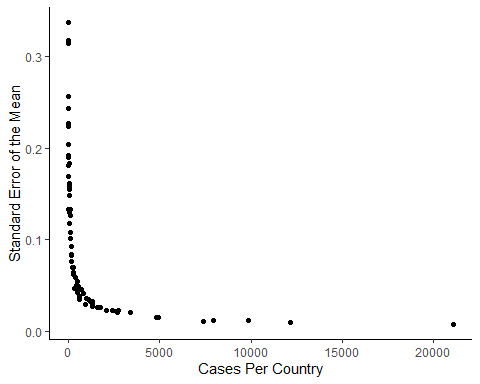
\includegraphics{02_ineq_risk_output_files/figure-latex/plot_case_numbers-1.pdf}

\begin{Shaded}
\begin{Highlighting}[]
\CommentTok{# ggplot(df, aes(x = reorder(iso, concern_self), y = concern_self)) + }
\CommentTok{#  geom_bar(stat = "identity") +}
\CommentTok{#  geom_errorbar(aes(ymin = ymin, ymax = ymax))}
\end{Highlighting}
\end{Shaded}

\hypertarget{additional-figs---residuals}{%
\paragraph{Additional Figs -
Residuals}\label{additional-figs---residuals}}

This visualizes the relationship between observed and predicted values
of risk perceptions and the regression results used for this prediction.

This introduces the difference between `over' and `under' concern with
the Coronavirus on average in a population.

\begin{Shaded}
\begin{Highlighting}[]
\CommentTok{# plot fitted v observed}
\KeywordTok{ggplot}\NormalTok{(df, }\KeywordTok{aes}\NormalTok{(}\DataTypeTok{y=}\NormalTok{m1p, }\DataTypeTok{x=}\NormalTok{concern_self)) }\OperatorTok{+}
\StringTok{  }\KeywordTok{geom_point}\NormalTok{() }\OperatorTok{+}
\StringTok{  }\KeywordTok{geom_text_repel}\NormalTok{(}\KeywordTok{aes}\NormalTok{(}\DataTypeTok{label=}\NormalTok{iso), }\DataTypeTok{vjust =} \FloatTok{1.5}\NormalTok{) }\OperatorTok{+}
\StringTok{  }\KeywordTok{geom_abline}\NormalTok{(}\DataTypeTok{slope=}\DecValTok{1}\NormalTok{) }\OperatorTok{+}

\StringTok{  }\KeywordTok{xlab}\NormalTok{(}\StringTok{"Observed Risk Perceptions"}\NormalTok{) }\OperatorTok{+}
\StringTok{  }\KeywordTok{ylab}\NormalTok{(}\StringTok{"Predicted Risk Perceptions"}\NormalTok{) }\OperatorTok{+}
\StringTok{  }\KeywordTok{theme_classic}\NormalTok{()}
\end{Highlighting}
\end{Shaded}

\begin{verbatim}
## Warning: ggrepel: 1 unlabeled data points (too many overlaps). Consider
## increasing max.overlaps
\end{verbatim}

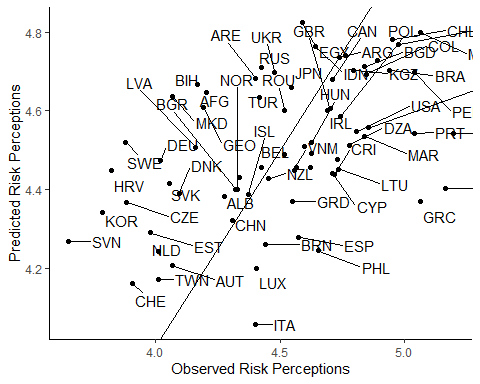
\includegraphics{02_ineq_risk_output_files/figure-latex/adjusted_risk-1.pdf}

\hypertarget{figure-3}{%
\paragraph{Figure 3}\label{figure-3}}

\begin{Shaded}
\begin{Highlighting}[]
\KeywordTok{agg_png}\NormalTok{(}\DataTypeTok{file =} \StringTok{"results/Fig3.png"}\NormalTok{, }\DataTypeTok{width =} \DecValTok{1000}\NormalTok{, }\DataTypeTok{height =} \DecValTok{600}\NormalTok{, }\DataTypeTok{res =} \DecValTok{144}\NormalTok{)}
\KeywordTok{ggplot}\NormalTok{(df, }\KeywordTok{aes}\NormalTok{(}\DataTypeTok{y=}\NormalTok{m1r, }\DataTypeTok{x=}\NormalTok{gini_disp)) }\OperatorTok{+}
\StringTok{  }\KeywordTok{geom_smooth}\NormalTok{(}\DataTypeTok{method=}\NormalTok{lm, }\DataTypeTok{se=}\NormalTok{T, }\DataTypeTok{size =} \FloatTok{0.3}\NormalTok{, }\DataTypeTok{color =} \StringTok{"gray30"}\NormalTok{) }\OperatorTok{+}
\StringTok{  }\KeywordTok{geom_text_repel}\NormalTok{(}\KeywordTok{aes}\NormalTok{(}\DataTypeTok{label=}\NormalTok{iso), }\DataTypeTok{size =} \DecValTok{3}\NormalTok{, }\DataTypeTok{color =} \StringTok{"blue4"}\NormalTok{, }\DataTypeTok{segment.size =} \FloatTok{0.1}\NormalTok{) }\OperatorTok{+}
\StringTok{  }\KeywordTok{xlab}\NormalTok{(}\StringTok{"Disposable Income Inequality"}\NormalTok{) }\OperatorTok{+}
\StringTok{  }\KeywordTok{ylab}\NormalTok{(}\StringTok{"Risk Perceptions (M1 residuals)"}\NormalTok{) }\OperatorTok{+}
\StringTok{  }\KeywordTok{labs}\NormalTok{(}\DataTypeTok{title =} \StringTok{""}\NormalTok{, }\DataTypeTok{subtitle =} \StringTok{"}\CharTok{\textbackslash{}'}\StringTok{Over}\CharTok{\textbackslash{}'}\StringTok{ or }\CharTok{\textbackslash{}'}\StringTok{under}\CharTok{\textbackslash{}'}\StringTok{ concern explained by income gini"}\NormalTok{) }\OperatorTok{+}
\StringTok{  }\KeywordTok{theme_classic}\NormalTok{() }\OperatorTok{+}\StringTok{ }
\StringTok{  }\KeywordTok{theme}\NormalTok{(}
  \DataTypeTok{plot.title =} \KeywordTok{element_text}\NormalTok{(),}
  \DataTypeTok{plot.subtitle =} \KeywordTok{element_text}\NormalTok{(}\DataTypeTok{face =} \StringTok{"italic"}\NormalTok{),}
  \DataTypeTok{plot.caption =} \KeywordTok{element_text}\NormalTok{(}\DataTypeTok{size =} \DecValTok{9}\NormalTok{, }\DataTypeTok{color =} \StringTok{"grey30"}\NormalTok{, }\DataTypeTok{vjust =} \FloatTok{-2.5}\NormalTok{),}
  \DataTypeTok{axis.title.x =} \KeywordTok{element_text}\NormalTok{(}\DataTypeTok{vjust =} \FloatTok{-0.8}\NormalTok{),}
  \DataTypeTok{axis.title.y =} \KeywordTok{element_text}\NormalTok{(}\DataTypeTok{vjust =} \DecValTok{2}\NormalTok{),}
\NormalTok{  )}
\end{Highlighting}
\end{Shaded}

\begin{verbatim}
## `geom_smooth()` using formula 'y ~ x'
\end{verbatim}

\begin{Shaded}
\begin{Highlighting}[]
\KeywordTok{invisible}\NormalTok{(}\KeywordTok{dev.off}\NormalTok{())}
\NormalTok{knitr}\OperatorTok{::}\KeywordTok{include_graphics}\NormalTok{(}\StringTok{"results/Fig3.png"}\NormalTok{)}
\end{Highlighting}
\end{Shaded}

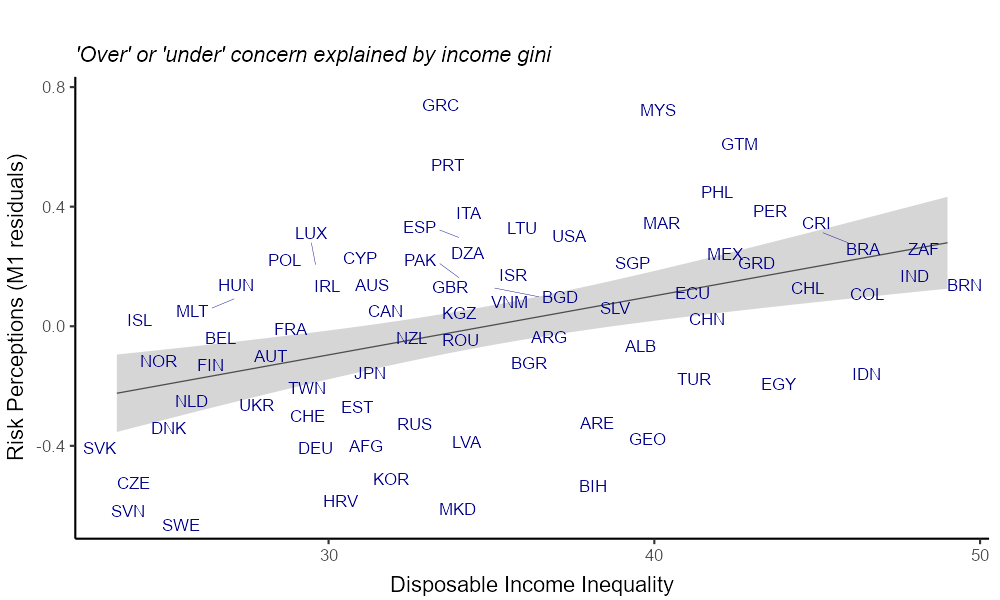
\includegraphics[width=13.89in]{results/Fig3}

\begin{Shaded}
\begin{Highlighting}[]
\CommentTok{#    }
\end{Highlighting}
\end{Shaded}

\hypertarget{additional-fig---3-way-plot}{%
\paragraph{Additional Fig - 3 Way
Plot}\label{additional-fig---3-way-plot}}

\begin{Shaded}
\begin{Highlighting}[]
\NormalTok{mid <-}\StringTok{ }\DecValTok{34}
\CommentTok{# trim gini to get better color display}
\NormalTok{df}\OperatorTok{$}\NormalTok{gini_color <-}\StringTok{ }\KeywordTok{ifelse}\NormalTok{(df}\OperatorTok{$}\NormalTok{gini_disp}\OperatorTok{<}\DecValTok{45}\NormalTok{, df}\OperatorTok{$}\NormalTok{gini_disp, }\DecValTok{45}\NormalTok{)}

\KeywordTok{ggplot}\NormalTok{(}\DataTypeTok{data=}\NormalTok{df, }\KeywordTok{aes}\NormalTok{(}\DataTypeTok{x=}\NormalTok{conf_delta, }\DataTypeTok{y=}\NormalTok{concern_self, }\DataTypeTok{color =}\NormalTok{ gini_color)) }\OperatorTok{+}
\StringTok{  }\KeywordTok{geom_point}\NormalTok{() }\OperatorTok{+}
\StringTok{  }\KeywordTok{geom_smooth}\NormalTok{(}\DataTypeTok{method=}\NormalTok{lm, }\DataTypeTok{se=}\OtherTok{FALSE}\NormalTok{, }\DataTypeTok{color =} \StringTok{"gray50"}\NormalTok{, }\DataTypeTok{linetype =} \StringTok{"dashed"}\NormalTok{) }\OperatorTok{+}
\StringTok{  }\KeywordTok{geom_text_repel}\NormalTok{(}\KeywordTok{aes}\NormalTok{(}\DataTypeTok{label =}\NormalTok{ iso), }\DataTypeTok{size =} \FloatTok{2.8}\NormalTok{) }\OperatorTok{+}
\StringTok{  }\KeywordTok{scale_color_gradient2}\NormalTok{(}\DataTypeTok{midpoint=}\NormalTok{mid, }\DataTypeTok{low=}\StringTok{"blue"}\NormalTok{, }\DataTypeTok{mid=}\StringTok{"gray55"}\NormalTok{, }\DataTypeTok{high=}\StringTok{"red"}\NormalTok{, }\DataTypeTok{space=}\StringTok{"Lab"}\NormalTok{) }\OperatorTok{+}
\StringTok{  }\KeywordTok{labs}\NormalTok{(}\DataTypeTok{x=} \StringTok{"New Case Rate, past week"}\NormalTok{, }\DataTypeTok{y =} \StringTok{"Risk Perceptions"}\NormalTok{, }\DataTypeTok{color =} \StringTok{"Income Inequality}\CharTok{\textbackslash{}n}\StringTok{(Gini, post}\CharTok{\textbackslash{}n}\StringTok{tax & transfer)"}\NormalTok{) }\OperatorTok{+}
\StringTok{      }\KeywordTok{theme}\NormalTok{(}\DataTypeTok{panel.background =} \KeywordTok{element_rect}\NormalTok{(}\DataTypeTok{fill =} \StringTok{"white"}\NormalTok{, }\DataTypeTok{colour =} \StringTok{"grey50"}\NormalTok{),}
        \DataTypeTok{panel.grid.major =} \KeywordTok{element_blank}\NormalTok{(),}
        \DataTypeTok{panel.grid.minor =} \KeywordTok{element_blank}\NormalTok{(),}
        \DataTypeTok{legend.title =} \KeywordTok{element_text}\NormalTok{(}\DataTypeTok{size =} \DecValTok{10}\NormalTok{))}
\end{Highlighting}
\end{Shaded}

\begin{verbatim}
## `geom_smooth()` using formula 'y ~ x'
\end{verbatim}

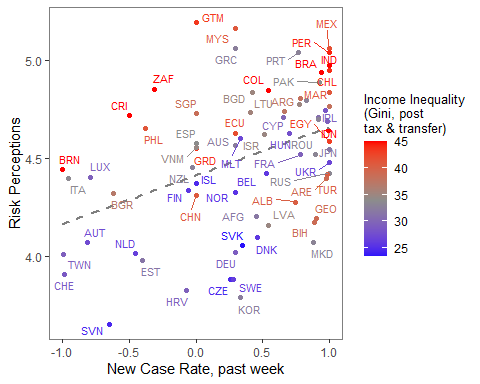
\includegraphics{02_ineq_risk_output_files/figure-latex/plot9-1.pdf}

\hypertarget{main-analyses}{%
\subsection{Main Analyses}\label{main-analyses}}

\hypertarget{predicting-risk-perceptions}{%
\subsubsection{Predicting Risk
Perceptions}\label{predicting-risk-perceptions}}

\hypertarget{table-1.-m1-through-m5}{%
\paragraph{Table 1. M1 through M5}\label{table-1.-m1-through-m5}}

So far this works to convert html to png
\url{https://cloudconvert.com/html-to-png}, but we should play around
with htmltools package to automate this in the code

\begin{Shaded}
\begin{Highlighting}[]
\CommentTok{#m1x <- lm(concern_self ~ days_since_peak + conf_delta + gov_resp*gov_resp_avg, data = df)}

\NormalTok{m2 <-}\StringTok{ }\KeywordTok{lm}\NormalTok{(concern_self }\OperatorTok{~}\StringTok{ }\NormalTok{days_since_peak }\OperatorTok{+}\StringTok{ }\NormalTok{conf_delta }\OperatorTok{+}\StringTok{ }\NormalTok{gov_resp }\OperatorTok{+}\StringTok{ }\NormalTok{gini_disp, }\DataTypeTok{data =}\NormalTok{ df)}

\CommentTok{# predicted values for sem}
\NormalTok{df}\OperatorTok{$}\NormalTok{m2p <-}\StringTok{ }\KeywordTok{predict.lm}\NormalTok{(m2, df)}

\CommentTok{# residuals}
\NormalTok{df}\OperatorTok{$}\NormalTok{m2r <-}\StringTok{ }\NormalTok{df}\OperatorTok{$}\NormalTok{concern_self }\OperatorTok{-}\StringTok{ }\NormalTok{df}\OperatorTok{$}\NormalTok{m2p }

\NormalTok{m3 <-}\StringTok{ }\KeywordTok{lm}\NormalTok{(concern_self }\OperatorTok{~}\StringTok{ }\NormalTok{days_since_peak }\OperatorTok{+}\StringTok{ }\NormalTok{conf_delta }\OperatorTok{+}\StringTok{ }\NormalTok{gov_resp }\OperatorTok{+}\StringTok{ }\NormalTok{socpolicy, }\DataTypeTok{data =}\NormalTok{ df)}

\NormalTok{m4 <-}\StringTok{ }\KeywordTok{lm}\NormalTok{(concern_self }\OperatorTok{~}\StringTok{ }\NormalTok{days_since_peak }\OperatorTok{+}\StringTok{ }\NormalTok{conf_delta }\OperatorTok{+}\StringTok{ }\NormalTok{gov_resp }\OperatorTok{+}\StringTok{ }\NormalTok{gdp, }\DataTypeTok{data =}\NormalTok{ df)}

\NormalTok{m5 <-}\StringTok{ }\KeywordTok{lm}\NormalTok{(concern_self }\OperatorTok{~}\StringTok{ }\NormalTok{days_since_peak }\OperatorTok{+}\StringTok{ }\NormalTok{conf_delta }\OperatorTok{+}\StringTok{ }\NormalTok{gov_resp }\OperatorTok{+}\StringTok{ }\NormalTok{gini_disp }\OperatorTok{+}\StringTok{ }\NormalTok{socpolicy }\OperatorTok{+}\StringTok{ }\NormalTok{gdp, }\DataTypeTok{data =}\NormalTok{ df)}


\KeywordTok{tab_model}\NormalTok{(m1, m2, m3, m4, m5, }\DataTypeTok{p.style =} \StringTok{"stars"}\NormalTok{, }\DataTypeTok{p.threshold =} \KeywordTok{c}\NormalTok{(}\FloatTok{0.10}\NormalTok{, }\FloatTok{0.05}\NormalTok{, }\FloatTok{0.01}\NormalTok{), }\DataTypeTok{show.ci =}\NormalTok{ F, }\DataTypeTok{rm.terms =} \KeywordTok{c}\NormalTok{(}\StringTok{"(Intercept)"}\NormalTok{), }\DataTypeTok{show.loglik =}\NormalTok{ T, }\DataTypeTok{show.aic =}\NormalTok{ T, }\DataTypeTok{dv.labels =} \KeywordTok{c}\NormalTok{(}\StringTok{"M1"}\NormalTok{, }\StringTok{"M2"}\NormalTok{,}\StringTok{"M3"}\NormalTok{, }\StringTok{"M4"}\NormalTok{,}\StringTok{"M5"}\NormalTok{), }\DataTypeTok{pred.labels =} \KeywordTok{c}\NormalTok{(}\StringTok{"Days Since Curve Inflection"}\NormalTok{, }\StringTok{"New Case Rate"}\NormalTok{, }\StringTok{"Government Intervention"}\NormalTok{, }\StringTok{"Disposable Income Inequality"}\NormalTok{, }\StringTok{"Welfare State Strength"}\NormalTok{, }\StringTok{"GDP Per Capita"}\NormalTok{), }\DataTypeTok{file =} \StringTok{"results/Tbl1.html"}\NormalTok{)}
\end{Highlighting}
\end{Shaded}

~

M1

M2

M3

M4

M5

Predictors

Estimates

Estimates

Estimates

Estimates

Estimates

Days Since Curve Inflection

-0.00 **

0.00

-0.00

-0.00

0.00

New Case Rate

0.18 ***

0.20 ***

0.18 ***

0.18 **

0.20 ***

Government Intervention

-0.04

-0.04

-0.05

-0.05

-0.04

Disposable Income Inequality

0.03 ***

0.03 ***

Welfare State Strength

-0.08 *

0.04

GDP Per Capita

-0.00

-0.00

Observations

74

74

74

74

74

R2 / R2 adjusted

0.238 / 0.206

0.427 / 0.393

0.277 / 0.235

0.262 / 0.219

0.433 / 0.382

AIC

47.802

28.783

45.915

47.492

31.982

log-Likelihood

-18.901

-8.392

-16.957

-17.746

-7.991

\begin{itemize}
\tightlist
\item
  p\textless0.1~~~** p\textless0.05~~~*** p\textless0.01
\end{itemize}

\hypertarget{standardized-coefficients-for-table-1}{%
\paragraph{Standardized Coefficients for Table
1}\label{standardized-coefficients-for-table-1}}

\begin{Shaded}
\begin{Highlighting}[]
\KeywordTok{tab_model}\NormalTok{(m1, m2, m3, m4, m5, }\DataTypeTok{p.style =} \StringTok{"stars"}\NormalTok{, }\DataTypeTok{p.threshold =} \KeywordTok{c}\NormalTok{(}\FloatTok{0.10}\NormalTok{, }\FloatTok{0.05}\NormalTok{, }\FloatTok{0.01}\NormalTok{), }\DataTypeTok{show.ci =}\NormalTok{ F, }\DataTypeTok{rm.terms =} \KeywordTok{c}\NormalTok{(}\StringTok{"(Intercept)"}\NormalTok{), }\DataTypeTok{show.std =}\NormalTok{ T, }\DataTypeTok{dv.labels =} \KeywordTok{c}\NormalTok{(}\StringTok{"M1_Z"}\NormalTok{, }\StringTok{"M2_Z"}\NormalTok{,}\StringTok{"M3_Z"}\NormalTok{, }\StringTok{"M4_Z"}\NormalTok{,}\StringTok{"M5_Z"}\NormalTok{), }\DataTypeTok{pred.labels =} \KeywordTok{c}\NormalTok{(}\StringTok{"Days Since Curve Inflection"}\NormalTok{, }\StringTok{"New Case Rate"}\NormalTok{, }\StringTok{"Government Intervention"}\NormalTok{, }\StringTok{"Disposable Income Inequality"}\NormalTok{, }\StringTok{"Welfare State Strength"}\NormalTok{, }\StringTok{"GDP Per Capita"}\NormalTok{))}
\end{Highlighting}
\end{Shaded}

~

M1\_Z

M2\_Z

M3\_Z

M4\_Z

M5\_Z

Predictors

Estimates

std. Beta

Estimates

std. Beta

Estimates

std. Beta

Estimates

std. Beta

Estimates

std. Beta

Days Since Curve Inflection

-0.00 **

-0.24

0.00

0.03

-0.00

-0.12

-0.00

-0.14

0.00

0.01

New Case Rate

0.18 ***

0.31

0.20 ***

0.33

0.18 ***

0.30

0.18 **

0.29

0.20 ***

0.34

Government Intervention

-0.04

-0.11

-0.04

-0.11

-0.05

-0.14

-0.05

-0.14

-0.04

-0.10

Disposable Income Inequality

0.03 ***

0.50

0.03 ***

0.57

Welfare State Strength

-0.08 *

-0.23

0.04

0.12

GDP Per Capita

-0.00

-0.19

-0.00

-0.03

Observations

74

74

74

74

74

R2 / R2 adjusted

0.238 / 0.206

0.427 / 0.393

0.277 / 0.235

0.262 / 0.219

0.433 / 0.382

\begin{itemize}
\tightlist
\item
  p\textless0.1~~~** p\textless0.05~~~*** p\textless0.01
\end{itemize}

\hypertarget{additional-table-m2_resid--the-regression-behind-fig-3}{%
\paragraph{Additional Table ``M2\_resid''- The Regression behind Fig
3}\label{additional-table-m2_resid--the-regression-behind-fig-3}}

\begin{Shaded}
\begin{Highlighting}[]
\NormalTok{m3r <-}\StringTok{ }\KeywordTok{lm}\NormalTok{(m1r }\OperatorTok{~}\StringTok{ }\NormalTok{days_since_peak }\OperatorTok{+}\StringTok{ }\NormalTok{conf_delta }\OperatorTok{+}\StringTok{ }\NormalTok{gov_resp }\OperatorTok{+}\StringTok{ }\NormalTok{gini_disp, }\DataTypeTok{data =}\NormalTok{ df)}

\KeywordTok{tab_model}\NormalTok{(m3r, }\DataTypeTok{p.style =} \StringTok{"stars"}\NormalTok{, }\DataTypeTok{p.threshold =} \KeywordTok{c}\NormalTok{(}\FloatTok{0.10}\NormalTok{, }\FloatTok{0.05}\NormalTok{, }\FloatTok{0.01}\NormalTok{), }\DataTypeTok{show.ci =}\NormalTok{ F, }\DataTypeTok{rm.terms =} \KeywordTok{c}\NormalTok{(}\StringTok{"(Intercept)"}\NormalTok{), }\DataTypeTok{show.std =}\NormalTok{ T, }\DataTypeTok{dv.labels =} \KeywordTok{c}\NormalTok{(}\StringTok{"M2_resid"}\NormalTok{), }\DataTypeTok{pred.labels =} \KeywordTok{c}\NormalTok{(}\StringTok{"Days Since Curve Inflection"}\NormalTok{, }\StringTok{"New Case Rate"}\NormalTok{, }\StringTok{"Intervention Severity"}\NormalTok{, }\StringTok{"Disposable Income Inequality"}\NormalTok{))}
\end{Highlighting}
\end{Shaded}

~

M2\_resid

Predictors

Estimates

std. Beta

Days Since Curve Inflection

0.00 **

0.30

New Case Rate

0.01

0.03

Intervention Severity

-0.00

-0.00

Disposable Income Inequality

0.03 ***

0.58

Observations

74

R2 / R2 adjusted

0.247 / 0.204

\begin{itemize}
\tightlist
\item
  p\textless0.1~~~** p\textless0.05~~~*** p\textless0.01
\end{itemize}

\hypertarget{additional-table---top-1-instead-of-gini}{%
\paragraph{Additional Table - Top 1\% instead of
Gini}\label{additional-table---top-1-instead-of-gini}}

\begin{Shaded}
\begin{Highlighting}[]
\CommentTok{# create dataset with top1 data cases only}

\NormalTok{dft <-}\StringTok{ }\NormalTok{df[(}\OperatorTok{!}\KeywordTok{is.na}\NormalTok{(df}\OperatorTok{$}\NormalTok{top1)),]}

\NormalTok{m1t <-}\StringTok{ }\KeywordTok{lm}\NormalTok{(concern_self }\OperatorTok{~}\StringTok{ }\NormalTok{days_since_peak }\OperatorTok{+}\StringTok{ }\NormalTok{conf_delta }\OperatorTok{+}\StringTok{ }\NormalTok{gov_resp, }\DataTypeTok{data =}\NormalTok{ dft)}

\NormalTok{m2t <-}\StringTok{ }\KeywordTok{lm}\NormalTok{(concern_self }\OperatorTok{~}\StringTok{ }\NormalTok{days_since_peak }\OperatorTok{+}\StringTok{ }\NormalTok{conf_delta }\OperatorTok{+}\StringTok{ }\NormalTok{gov_resp }\OperatorTok{+}\StringTok{ }\NormalTok{top1, }\DataTypeTok{data =}\NormalTok{ dft)}

\NormalTok{m3t <-}\StringTok{ }\KeywordTok{lm}\NormalTok{(concern_self }\OperatorTok{~}\StringTok{ }\NormalTok{days_since_peak }\OperatorTok{+}\StringTok{ }\NormalTok{conf_delta }\OperatorTok{+}\StringTok{ }\NormalTok{gov_resp }\OperatorTok{+}\StringTok{ }\NormalTok{socpolicy, }\DataTypeTok{data =}\NormalTok{ dft)}

\NormalTok{m4t <-}\StringTok{ }\KeywordTok{lm}\NormalTok{(concern_self }\OperatorTok{~}\StringTok{ }\NormalTok{days_since_peak }\OperatorTok{+}\StringTok{ }\NormalTok{conf_delta }\OperatorTok{+}\StringTok{ }\NormalTok{gov_resp }\OperatorTok{+}\StringTok{ }\NormalTok{gdp, }\DataTypeTok{data =}\NormalTok{ dft)}

\NormalTok{m5t <-}\StringTok{ }\KeywordTok{lm}\NormalTok{(concern_self }\OperatorTok{~}\StringTok{ }\NormalTok{days_since_peak }\OperatorTok{+}\StringTok{ }\NormalTok{conf_delta }\OperatorTok{+}\StringTok{ }\NormalTok{gov_resp }\OperatorTok{+}\StringTok{ }\NormalTok{top1 }\OperatorTok{+}\StringTok{ }\NormalTok{socpolicy }\OperatorTok{+}\StringTok{ }\NormalTok{gdp, }\DataTypeTok{data =}\NormalTok{ dft)}

\KeywordTok{tab_model}\NormalTok{(m1t, m2t, m3t, m4t, m5t, }\DataTypeTok{p.style =} \StringTok{"stars"}\NormalTok{, }\DataTypeTok{p.threshold =} \KeywordTok{c}\NormalTok{(}\FloatTok{0.10}\NormalTok{, }\FloatTok{0.05}\NormalTok{, }\FloatTok{0.01}\NormalTok{), }\DataTypeTok{show.ci =}\NormalTok{ F, }\DataTypeTok{rm.terms =} \KeywordTok{c}\NormalTok{(}\StringTok{"(Intercept)"}\NormalTok{), }\DataTypeTok{show.loglik =}\NormalTok{ T, }\DataTypeTok{show.aic =}\NormalTok{ T, }\DataTypeTok{dv.labels =} \KeywordTok{c}\NormalTok{(}\StringTok{"M11"}\NormalTok{, }\StringTok{"M12"}\NormalTok{,}\StringTok{"M13"}\NormalTok{, }\StringTok{"M14"}\NormalTok{,}\StringTok{"M15"}\NormalTok{), }\DataTypeTok{pred.labels =} \KeywordTok{c}\NormalTok{(}\StringTok{"Days Since Curve Inflection"}\NormalTok{, }\StringTok{"New Case Rate"}\NormalTok{, }\StringTok{"Government Intervention"}\NormalTok{, }\StringTok{"Top 1% Income Concentration"}\NormalTok{, }\StringTok{"Welfare State Strength"}\NormalTok{, }\StringTok{"GDP Per Capita"}\NormalTok{))}
\end{Highlighting}
\end{Shaded}

~

M11

M12

M13

M14

M15

Predictors

Estimates

Estimates

Estimates

Estimates

Estimates

Days Since Curve Inflection

-0.00

0.00

-0.00

-0.00

0.00

New Case Rate

0.27 ***

0.22 ***

0.25 ***

0.25 ***

0.20 **

Government Intervention

-0.06

-0.03

-0.06

-0.07

-0.04

Top 1\% Income Concentration

2.78 ***

2.75 **

Welfare State Strength

-0.05

-0.01

GDP Per Capita

-0.00

-0.00

Observations

57

57

57

57

57

R2 / R2 adjusted

0.270 / 0.229

0.363 / 0.314

0.286 / 0.231

0.278 / 0.222

0.374 / 0.298

AIC

38.338

32.563

39.074

39.732

35.628

log-Likelihood

-14.169

-10.282

-13.537

-13.866

-9.814

\begin{itemize}
\tightlist
\item
  p\textless0.1~~~** p\textless0.05~~~*** p\textless0.01
\end{itemize}

\hypertarget{additional-table---standardized-results-for-above}{%
\paragraph{Additional Table - Standardized Results for
above}\label{additional-table---standardized-results-for-above}}

\begin{Shaded}
\begin{Highlighting}[]
\KeywordTok{tab_model}\NormalTok{(m1t, m2t, m3t, m4t, m5t, }\DataTypeTok{p.style =} \StringTok{"stars"}\NormalTok{, }\DataTypeTok{p.threshold =} \KeywordTok{c}\NormalTok{(}\FloatTok{0.10}\NormalTok{, }\FloatTok{0.05}\NormalTok{, }\FloatTok{0.01}\NormalTok{), }\DataTypeTok{show.ci =}\NormalTok{ F, }\DataTypeTok{rm.terms =} \KeywordTok{c}\NormalTok{(}\StringTok{"(Intercept)"}\NormalTok{), }\DataTypeTok{show.std =}\NormalTok{ T, }\DataTypeTok{dv.labels =} \KeywordTok{c}\NormalTok{(}\StringTok{"M11_Z"}\NormalTok{, }\StringTok{"M12_Z"}\NormalTok{,}\StringTok{"M13_Z"}\NormalTok{, }\StringTok{"M14_Z"}\NormalTok{,}\StringTok{"M15_Z"}\NormalTok{), }\DataTypeTok{pred.labels =} \KeywordTok{c}\NormalTok{(}\StringTok{"Days Since Curve Inflection"}\NormalTok{, }\StringTok{"New Case Rate"}\NormalTok{, }\StringTok{"Intervention Severity"}\NormalTok{, }\StringTok{"Top 1% Income Concentration"}\NormalTok{, }\StringTok{"Welfare State Strength"}\NormalTok{, }\StringTok{"GDP Per Capita"}\NormalTok{))}
\end{Highlighting}
\end{Shaded}

~

M11\_Z

M12\_Z

M13\_Z

M14\_Z

M15\_Z

Predictors

Estimates

std. Beta

Estimates

std. Beta

Estimates

std. Beta

Estimates

std. Beta

Estimates

std. Beta

Days Since Curve Inflection

-0.00

-0.07

0.00

0.05

-0.00

-0.02

-0.00

-0.04

0.00

0.10

New Case Rate

0.27 ***

0.44

0.22 ***

0.36

0.25 ***

0.42

0.25 ***

0.42

0.20 **

0.33

Intervention Severity

-0.06

-0.16

-0.03

-0.08

-0.06

-0.17

-0.07

-0.18

-0.04

-0.10

Top 1\% Income Concentration

2.78 ***

0.37

2.75 **

0.36

Welfare State Strength

-0.05

-0.14

-0.01

-0.03

GDP Per Capita

-0.00

-0.10

-0.00

-0.10

Observations

57

57

57

57

57

R2 / R2 adjusted

0.270 / 0.229

0.363 / 0.314

0.286 / 0.231

0.278 / 0.222

0.374 / 0.298

\begin{itemize}
\tightlist
\item
  p\textless0.1~~~** p\textless0.05~~~*** p\textless0.01
\end{itemize}

\hypertarget{predicting-infection-increase-ratio-may-1---may-31}{%
\subsubsection{Predicting Infection Increase (ratio), May 1 - May
31}\label{predicting-infection-increase-ratio-may-1---may-31}}

Conf\_delta (new cases) measures a type of information the public and
media consumes, it is actually a cause of a lower increase ratio of
infection, probably because having awareness of a high infection
increase leads to behavioral and policy changes.

\hypertarget{additional-table.-infection-increase-as-dv}{%
\paragraph{Additional Table. Infection Increase as
DV}\label{additional-table.-infection-increase-as-dv}}

These are the OLS analyses that mirror those in Table 2, but without ML
simultaneous estimation. Here OLS is our `first run', but it is biased
because it cannot estimate mediation effects and therefore M40-M43 (and
M50-M53 with top 1\%) are the preferred models due to maximum-likelihood
estimation.

\begin{Shaded}
\begin{Highlighting}[]
\NormalTok{m21 <-}\StringTok{ }\KeywordTok{lm}\NormalTok{(rate_}\DecValTok{2} \OperatorTok{~}\StringTok{ }\NormalTok{days_since_peak }\OperatorTok{+}\StringTok{ }\NormalTok{conf_delta }\OperatorTok{+}\StringTok{ }\NormalTok{gov_resp , }\DataTypeTok{data =}\NormalTok{ df)}

\NormalTok{m22 <-}\StringTok{ }\KeywordTok{lm}\NormalTok{(rate_}\DecValTok{2} \OperatorTok{~}\StringTok{ }\NormalTok{days_since_peak }\OperatorTok{+}\StringTok{ }\NormalTok{conf_delta }\OperatorTok{+}\StringTok{ }\NormalTok{gov_resp }\OperatorTok{+}\StringTok{ }\NormalTok{concern_self, }\DataTypeTok{data =}\NormalTok{ df)}

\NormalTok{m23 <-}\StringTok{ }\KeywordTok{lm}\NormalTok{(rate_}\DecValTok{2} \OperatorTok{~}\StringTok{ }\NormalTok{days_since_peak }\OperatorTok{+}\StringTok{ }\NormalTok{conf_delta }\OperatorTok{+}\StringTok{ }\NormalTok{gov_resp }\OperatorTok{+}\StringTok{ }\NormalTok{concern_self }\OperatorTok{+}\StringTok{ }\KeywordTok{I}\NormalTok{(concern_self}\OperatorTok{^}\DecValTok{2}\NormalTok{), }\DataTypeTok{data =}\NormalTok{ df)}

\NormalTok{m24 <-}\StringTok{ }\KeywordTok{lm}\NormalTok{(rate_}\DecValTok{2} \OperatorTok{~}\StringTok{ }\NormalTok{days_since_peak }\OperatorTok{+}\StringTok{ }\NormalTok{conf_delta }\OperatorTok{+}\StringTok{ }\NormalTok{gov_resp }\OperatorTok{+}\StringTok{  }\NormalTok{gini_disp, }\DataTypeTok{data =}\NormalTok{ df)}

\NormalTok{m25 <-}\StringTok{ }\KeywordTok{lm}\NormalTok{(rate_}\DecValTok{2} \OperatorTok{~}\StringTok{ }\NormalTok{days_since_peak }\OperatorTok{+}\StringTok{ }\NormalTok{conf_delta }\OperatorTok{+}\StringTok{ }\NormalTok{gov_resp }\OperatorTok{+}\StringTok{ }\NormalTok{concern_self }\OperatorTok{+}\StringTok{ }\NormalTok{gini_disp, }\DataTypeTok{data =}\NormalTok{ df)}

\NormalTok{m26 <-}\StringTok{ }\KeywordTok{lm}\NormalTok{(rate_}\DecValTok{2} \OperatorTok{~}\StringTok{ }\NormalTok{days_since_peak }\OperatorTok{+}\StringTok{ }\NormalTok{conf_delta }\OperatorTok{+}\StringTok{ }\NormalTok{gov_resp }\OperatorTok{+}\StringTok{ }\NormalTok{gini_disp }\OperatorTok{+}\StringTok{ }\KeywordTok{I}\NormalTok{(gini_disp}\OperatorTok{^}\DecValTok{2}\NormalTok{), }\DataTypeTok{data =}\NormalTok{ df)}

\NormalTok{m27 <-}\StringTok{ }\KeywordTok{lm}\NormalTok{(rate_}\DecValTok{2} \OperatorTok{~}\StringTok{ }\NormalTok{days_since_peak }\OperatorTok{+}\StringTok{ }\NormalTok{conf_delta }\OperatorTok{+}\StringTok{ }\NormalTok{gov_resp }\OperatorTok{+}\StringTok{  }\NormalTok{concern_self }\OperatorTok{+}\StringTok{ }\KeywordTok{I}\NormalTok{(concern_self}\OperatorTok{^}\DecValTok{2}\NormalTok{) }\OperatorTok{+}\StringTok{ }\NormalTok{gini_disp }\OperatorTok{+}\StringTok{ }\KeywordTok{I}\NormalTok{(gini_disp}\OperatorTok{^}\DecValTok{2}\NormalTok{), }\DataTypeTok{data =}\NormalTok{ df)}



\KeywordTok{tab_model}\NormalTok{(m21, m22, m23, m24, m25, m26, m27, }\DataTypeTok{p.style =} \StringTok{"stars"}\NormalTok{, }\DataTypeTok{p.threshold =} \KeywordTok{c}\NormalTok{(}\FloatTok{0.10}\NormalTok{, }\FloatTok{0.05}\NormalTok{, }\FloatTok{0.01}\NormalTok{), }\DataTypeTok{show.ci =}\NormalTok{ F, }\DataTypeTok{rm.terms =} \KeywordTok{c}\NormalTok{(}\StringTok{"(Intercept)"}\NormalTok{), }\DataTypeTok{show.loglik =}\NormalTok{ T, }\DataTypeTok{show.aic =}\NormalTok{ T, }\DataTypeTok{dv.labels =} \KeywordTok{c}\NormalTok{(}\StringTok{"M21"}\NormalTok{, }\StringTok{"M22"}\NormalTok{,}\StringTok{"M23"}\NormalTok{, }\StringTok{"M24"}\NormalTok{,}\StringTok{"M25"}\NormalTok{,}\StringTok{"M26"}\NormalTok{,}\StringTok{"M27"}\NormalTok{), }\DataTypeTok{pred.labels =} \KeywordTok{c}\NormalTok{(}\StringTok{"Days Since Curve Inflection"}\NormalTok{, }\StringTok{"New Case Rate"}\NormalTok{, }\StringTok{"Government Intervention"}\NormalTok{, }\StringTok{"Risk Perceptions"}\NormalTok{, }\StringTok{"Risk Perceptions^2"}\NormalTok{, }\StringTok{"Disposable Income Inequality"}\NormalTok{, }\StringTok{"Disposable Income Inequality^2"}\NormalTok{))}
\end{Highlighting}
\end{Shaded}

~

M21

M22

M23

M24

M25

M26

M27

Predictors

Estimates

Estimates

Estimates

Estimates

Estimates

Estimates

Estimates

Days Since Curve Inflection

-0.03 ***

-0.03 ***

-0.03 ***

-0.03 ***

-0.03 ***

-0.03 ***

-0.03 ***

New Case Rate

-0.10

-0.21 *

-0.18

-0.09

-0.18

-0.03

-0.10

Government Intervention

-0.15 **

-0.13 **

-0.09

-0.16 **

-0.14 **

-0.15 **

-0.10 *

Risk Perceptions

0.60 ***

-10.87 ***

0.45 **

-10.07 ***

Risk Perceptions\^{}2

1.29 ***

1.18 ***

Disposable Income Inequality

0.03 ***

0.02

-0.13

-0.12

Disposable Income Inequality\^{}2

0.00

0.00

Observations

74

74

74

74

74

74

74

R2 / R2 adjusted

0.631 / 0.615

0.675 / 0.656

0.718 / 0.698

0.665 / 0.645

0.684 / 0.660

0.677 / 0.654

0.735 / 0.707

AIC

128.460

121.002

112.397

123.274

121.030

122.469

111.901

log-Likelihood

-59.230

-54.501

-49.198

-55.637

-53.515

-54.235

-46.951

\begin{itemize}
\tightlist
\item
  p\textless0.1~~~** p\textless0.05~~~*** p\textless0.01
\end{itemize}

\begin{Shaded}
\begin{Highlighting}[]
\NormalTok{m27_beta <-}\StringTok{ }\KeywordTok{lm.beta}\NormalTok{(m27)}
\NormalTok{m27_beta_concern <-}\StringTok{ }\NormalTok{m27_beta[[}\StringTok{"standardized.coefficients"}\NormalTok{]][[}\StringTok{"concern_self"}\NormalTok{]] }\OperatorTok{+}\StringTok{ }\NormalTok{m27_beta[[}\StringTok{"standardized.coefficients"}\NormalTok{]][[}\StringTok{"I(concern_self^2)"}\NormalTok{]]}

\NormalTok{m27_beta_gini <-}\StringTok{ }\NormalTok{m27_beta[[}\StringTok{"standardized.coefficients"}\NormalTok{]][[}\StringTok{"gini_disp"}\NormalTok{]] }\OperatorTok{+}\StringTok{ }\NormalTok{m27_beta[[}\StringTok{"standardized.coefficients"}\NormalTok{]][[}\StringTok{"I(gini_disp^2)"}\NormalTok{]]}
\end{Highlighting}
\end{Shaded}

\hypertarget{standardized-coefficients-m27}{%
\paragraph{Standardized Coefficients
M27}\label{standardized-coefficients-m27}}

Standardized combined effect of term + term\^{}2

Risk Perceptions = Disposable Income Inequality =

\hypertarget{additional-table.-infection-increase-as-dv-using-top-1-instead.}{%
\paragraph{Additional Table. Infection Increase as DV Using Top 1\%
instead.}\label{additional-table.-infection-increase-as-dv-using-top-1-instead.}}

\begin{Shaded}
\begin{Highlighting}[]
\NormalTok{m31 <-}\StringTok{ }\KeywordTok{lm}\NormalTok{(rate_}\DecValTok{2} \OperatorTok{~}\StringTok{ }\NormalTok{days_since_peak }\OperatorTok{+}\StringTok{ }\NormalTok{conf_delta }\OperatorTok{+}\StringTok{ }\NormalTok{gov_resp , }\DataTypeTok{data =}\NormalTok{ dft)}

\NormalTok{m32 <-}\StringTok{ }\KeywordTok{lm}\NormalTok{(rate_}\DecValTok{2} \OperatorTok{~}\StringTok{ }\NormalTok{days_since_peak }\OperatorTok{+}\StringTok{ }\NormalTok{conf_delta }\OperatorTok{+}\StringTok{ }\NormalTok{gov_resp }\OperatorTok{+}\StringTok{ }\NormalTok{concern_self, }\DataTypeTok{data =}\NormalTok{ dft)}

\NormalTok{m33 <-}\StringTok{ }\KeywordTok{lm}\NormalTok{(rate_}\DecValTok{2} \OperatorTok{~}\StringTok{ }\NormalTok{days_since_peak }\OperatorTok{+}\StringTok{ }\NormalTok{conf_delta }\OperatorTok{+}\StringTok{ }\NormalTok{gov_resp }\OperatorTok{+}\StringTok{ }\NormalTok{concern_self }\OperatorTok{+}\StringTok{ }\KeywordTok{I}\NormalTok{(concern_self}\OperatorTok{^}\DecValTok{2}\NormalTok{), }\DataTypeTok{data =}\NormalTok{ dft)}

\NormalTok{m34 <-}\StringTok{ }\KeywordTok{lm}\NormalTok{(rate_}\DecValTok{2} \OperatorTok{~}\StringTok{ }\NormalTok{days_since_peak }\OperatorTok{+}\StringTok{ }\NormalTok{conf_delta }\OperatorTok{+}\StringTok{ }\NormalTok{gov_resp }\OperatorTok{+}\StringTok{  }\NormalTok{top1, }\DataTypeTok{data =}\NormalTok{ dft)}

\NormalTok{m35 <-}\StringTok{ }\KeywordTok{lm}\NormalTok{(rate_}\DecValTok{2} \OperatorTok{~}\StringTok{ }\NormalTok{days_since_peak }\OperatorTok{+}\StringTok{ }\NormalTok{conf_delta }\OperatorTok{+}\StringTok{ }\NormalTok{gov_resp }\OperatorTok{+}\StringTok{ }\NormalTok{concern_self }\OperatorTok{+}\StringTok{ }\NormalTok{top1, }\DataTypeTok{data =}\NormalTok{ df)}

\NormalTok{m36 <-}\StringTok{ }\KeywordTok{lm}\NormalTok{(rate_}\DecValTok{2} \OperatorTok{~}\StringTok{ }\NormalTok{days_since_peak }\OperatorTok{+}\StringTok{ }\NormalTok{conf_delta }\OperatorTok{+}\StringTok{ }\NormalTok{gov_resp }\OperatorTok{+}\StringTok{ }\NormalTok{top1 }\OperatorTok{+}\StringTok{ }\KeywordTok{I}\NormalTok{(top1}\OperatorTok{^}\DecValTok{2}\NormalTok{), }\DataTypeTok{data =}\NormalTok{ dft)}

\NormalTok{m37 <-}\StringTok{ }\KeywordTok{lm}\NormalTok{(rate_}\DecValTok{2} \OperatorTok{~}\StringTok{ }\NormalTok{days_since_peak }\OperatorTok{+}\StringTok{ }\NormalTok{conf_delta }\OperatorTok{+}\StringTok{ }\NormalTok{gov_resp }\OperatorTok{+}\StringTok{  }\NormalTok{concern_self }\OperatorTok{+}\StringTok{ }\KeywordTok{I}\NormalTok{(concern_self}\OperatorTok{^}\DecValTok{2}\NormalTok{) }\OperatorTok{+}\StringTok{ }\NormalTok{top1 }\OperatorTok{+}\StringTok{ }\KeywordTok{I}\NormalTok{(top1}\OperatorTok{^}\DecValTok{2}\NormalTok{), }\DataTypeTok{data =}\NormalTok{ dft)}

\KeywordTok{tab_model}\NormalTok{(m31, m32, m33, m34, m35, m36, m37, }\DataTypeTok{p.style =} \StringTok{"stars"}\NormalTok{, }\DataTypeTok{p.threshold =} \KeywordTok{c}\NormalTok{(}\FloatTok{0.10}\NormalTok{, }\FloatTok{0.05}\NormalTok{, }\FloatTok{0.01}\NormalTok{), }\DataTypeTok{show.ci =}\NormalTok{ F, }\DataTypeTok{rm.terms =} \KeywordTok{c}\NormalTok{(}\StringTok{"(Intercept)"}\NormalTok{), }\DataTypeTok{show.loglik =}\NormalTok{ T, }\DataTypeTok{show.aic =}\NormalTok{ T, }\DataTypeTok{dv.labels =} \KeywordTok{c}\NormalTok{(}\StringTok{"M31"}\NormalTok{, }\StringTok{"M32"}\NormalTok{,}\StringTok{"M33"}\NormalTok{, }\StringTok{"M34"}\NormalTok{,}\StringTok{"M35"}\NormalTok{,}\StringTok{"M36"}\NormalTok{, }\StringTok{"M37"}\NormalTok{), }\DataTypeTok{pred.labels =} \KeywordTok{c}\NormalTok{(}\StringTok{"Days Since Curve Inflection"}\NormalTok{, }\StringTok{"New Case Rate"}\NormalTok{, }\StringTok{"Government Intervention"}\NormalTok{, }\StringTok{"Risk Perceptions"}\NormalTok{, }\StringTok{"Risk Perceptions^2"}\NormalTok{, }\StringTok{"Disposable Income Inequality"}\NormalTok{, }\StringTok{"Disposable Income Inequality^2"}\NormalTok{))}
\end{Highlighting}
\end{Shaded}

~

M31

M32

M33

M34

M35

M36

M37

Predictors

Estimates

Estimates

Estimates

Estimates

Estimates

Estimates

Estimates

Days Since Curve Inflection

-0.03 ***

-0.03 ***

-0.03 ***

-0.03 ***

-0.03 ***

-0.03 ***

-0.03 ***

New Case Rate

-0.03

-0.17

-0.14

-0.14

-0.20 *

-0.13

-0.18

Government Intervention

-0.11

-0.07

-0.05

-0.04

-0.03

-0.05

-0.02

Risk Perceptions

0.51 **

-8.48 **

0.29

-6.52 *

Risk Perceptions\^{}2

1.02 **

0.78 *

Disposable Income Inequality

5.67 ***

4.87 ***

0.96

-0.87

Disposable Income Inequality\^{}2

15.40

16.88

Observations

57

57

57

57

57

57

57

R2 / R2 adjusted

0.622 / 0.601

0.666 / 0.640

0.699 / 0.670

0.710 / 0.688

0.722 / 0.695

0.713 / 0.685

0.747 / 0.711

AIC

85.389

80.449

76.373

72.373

71.958

73.723

70.580

log-Likelihood

-37.695

-34.224

-31.186

-30.186

-28.979

-29.861

-26.290

\begin{itemize}
\tightlist
\item
  p\textless0.1~~~** p\textless0.05~~~*** p\textless0.01
\end{itemize}

\hypertarget{standardized-coefficients-m37}{%
\paragraph{Standardized Coefficients
M37}\label{standardized-coefficients-m37}}

\begin{Shaded}
\begin{Highlighting}[]
\NormalTok{m37_beta <-}\StringTok{ }\KeywordTok{lm.beta}\NormalTok{(m37)}
\NormalTok{m37_beta_concern <-}\StringTok{ }\NormalTok{m37_beta[[}\StringTok{"standardized.coefficients"}\NormalTok{]][[}\StringTok{"concern_self"}\NormalTok{]] }\OperatorTok{+}\StringTok{ }\NormalTok{m37_beta[[}\StringTok{"standardized.coefficients"}\NormalTok{]][[}\StringTok{"I(concern_self^2)"}\NormalTok{]]}

\NormalTok{m37_beta_gini <-}\StringTok{ }\NormalTok{m37_beta[[}\StringTok{"standardized.coefficients"}\NormalTok{]][[}\StringTok{"top1"}\NormalTok{]] }\OperatorTok{+}\StringTok{ }\NormalTok{m37_beta[[}\StringTok{"standardized.coefficients"}\NormalTok{]][[}\StringTok{"I(top1^2)"}\NormalTok{]]}
\end{Highlighting}
\end{Shaded}

Standardized combined effect of term + term\^{}2

Risk Perceptions = Disposable Income Inequality =

\hypertarget{mediation-analysis}{%
\subsubsection{Mediation Analysis}\label{mediation-analysis}}

SEM squared variables must be constructed by hand. To keep estimates
`under control', it is useful to center the variables.

\hypertarget{m40-baseline-model}{%
\paragraph{M40 Baseline Model}\label{m40-baseline-model}}

This is a maximum-likelihood estimated combination of M1 and M23, i.e.,
a structural equation model.

\begin{Shaded}
\begin{Highlighting}[]
\NormalTok{m40 <-}\StringTok{ '     rate_2 ~ days_since_peak + conf_delta + gov_resp + concern_self + b2*concern_self2  + c1*gini_dispR + c2*gini_disp2}
\StringTok{             concern_self ~ days_since_peak + conf_delta + gov_resp + a1*gini_dispR + a2*gini_disp2}
\StringTok{           # this is critical because we constructed one out of the other   }
\StringTok{             concern_self2 ~ concern_self}
\StringTok{           # covariances}

\StringTok{           # intercepts}
\StringTok{             rate_2 ~ 1}
\StringTok{             concern_self ~ 1}
\StringTok{           # constraints}
\StringTok{             c1 == 0}
\StringTok{             c2 == 0}
\StringTok{             b2 == 0}
\StringTok{             a1 == 0}
\StringTok{             a2 == 0}
\StringTok{         '}
\NormalTok{m40fit <-}\StringTok{ }\KeywordTok{sem}\NormalTok{(m40, }\DataTypeTok{data =}\NormalTok{ df)}
\KeywordTok{summary}\NormalTok{(m40fit, }\DataTypeTok{fit.measures =}\NormalTok{ T)}
\end{Highlighting}
\end{Shaded}

\begin{verbatim}
## lavaan 0.6-7 ended normally after 76 iterations
## 
##   Estimator                                         ML
##   Optimization method                           NLMINB
##   Number of free parameters                         19
##   Number of equality constraints                     5
##                                                       
##   Number of observations                            74
##                                                       
## Model Test User Model:
##                                                       
##   Test statistic                                41.957
##   Degrees of freedom                                10
##   P-value (Chi-square)                           0.000
## 
## Model Test Baseline Model:
## 
##   Test statistic                               741.545
##   Degrees of freedom                                18
##   P-value                                        0.000
## 
## User Model versus Baseline Model:
## 
##   Comparative Fit Index (CFI)                    0.956
##   Tucker-Lewis Index (TLI)                       0.920
## 
## Loglikelihood and Information Criteria:
## 
##   Loglikelihood user model (H0)                -36.505
##   Loglikelihood unrestricted model (H1)        -15.526
##                                                       
##   Akaike (AIC)                                 101.010
##   Bayesian (BIC)                               133.267
##   Sample-size adjusted Bayesian (BIC)           89.147
## 
## Root Mean Square Error of Approximation:
## 
##   RMSEA                                          0.208
##   90 Percent confidence interval - lower         0.145
##   90 Percent confidence interval - upper         0.275
##   P-value RMSEA <= 0.05                          0.000
## 
## Standardized Root Mean Square Residual:
## 
##   SRMR                                           0.116
## 
## Parameter Estimates:
## 
##   Standard errors                             Standard
##   Information                                 Expected
##   Information saturated (h1) model          Structured
## 
## Regressions:
##                    Estimate  Std.Err  z-value  P(>|z|)
##   rate_2 ~                                            
##     dys_snc_p        -0.032    0.003   -9.526    0.000
##     conf_delt        -0.215    0.112   -1.912    0.056
##     gov_resp         -0.130    0.061   -2.149    0.032
##     cncrn_slf         0.597    0.188    3.176    0.001
##     cncrn_sl2 (b2)    0.000                           
##     gini_dspR (c1)    0.000       NA                  
##     gini_dsp2 (c2)    0.000                           
##   concern_self ~                                      
##     dys_snc_p        -0.004    0.002   -2.156    0.031
##     conf_delt         0.185    0.066    2.799    0.005
##     gov_resp         -0.039    0.037   -1.043    0.297
##     gini_dspR (a1)    0.000       NA                  
##     gini_dsp2 (a2)    0.000       NA                  
##   concern_self2 ~                                     
##     cncrn_slf         8.900    0.048  186.460    0.000
## 
## Intercepts:
##                    Estimate  Std.Err  z-value  P(>|z|)
##    .rate_2           -0.955    0.870   -1.097    0.273
##    .concern_self      4.572    0.084   54.532    0.000
##    .concern_self2   -19.670    0.216  -91.217    0.000
## 
## Variances:
##                    Estimate  Std.Err  z-value  P(>|z|)
##    .rate_2            0.255    0.042    6.083    0.000
##    .concern_self      0.098    0.016    6.083    0.000
##    .concern_self2     0.022    0.004    6.083    0.000
## 
## Constraints:
##                                                |Slack|
##     c1 - 0                                       0.000
##     c2 - 0                                       0.000
##     b2 - 0                                       0.000
##     a1 - 0                                       0.000
##     a2 - 0                                       0.000
\end{verbatim}

\begin{Shaded}
\begin{Highlighting}[]
\KeywordTok{standardizedsolution}\NormalTok{(m40fit)}
\end{Highlighting}
\end{Shaded}

\begin{verbatim}
##                lhs op             rhs est.std    se        z pvalue ci.lower
## 1           rate_2  ~ days_since_peak  -0.713 0.057  -12.591  0.000   -0.824
## 2           rate_2  ~      conf_delta  -0.145 0.075   -1.929  0.054   -0.292
## 3           rate_2  ~        gov_resp  -0.146 0.067   -2.173  0.030   -0.278
## 4           rate_2  ~    concern_self   0.241 0.076    3.180  0.001    0.093
## 5           rate_2  ~   concern_self2   0.000 0.003    0.000  1.000   -0.006
## 6           rate_2  ~      gini_dispR   0.000 0.000    0.000  1.000    0.000
## 7           rate_2  ~      gini_disp2   0.000 0.000    0.000  1.000    0.000
## 8     concern_self  ~ days_since_peak  -0.240 0.107   -2.230  0.026   -0.450
## 9     concern_self  ~      conf_delta   0.308 0.104    2.969  0.003    0.105
## 10    concern_self  ~        gov_resp  -0.108 0.102   -1.051  0.293   -0.309
## 11    concern_self  ~      gini_dispR   0.000 0.000    0.000  1.000    0.000
## 12    concern_self  ~      gini_disp2   0.000 0.000    0.000  1.000    0.000
## 13   concern_self2  ~    concern_self   0.999 0.000 4104.510  0.000    0.998
## 14          rate_2 ~1                  -1.077 0.975   -1.104  0.270   -2.989
## 15    concern_self ~1                  12.772 1.022   12.498  0.000   10.769
## 16          rate_2 ~~          rate_2   0.325 0.052    6.232  0.000    0.223
## 17    concern_self ~~    concern_self   0.762 0.081    9.387  0.000    0.603
## 18   concern_self2 ~~   concern_self2   0.002 0.000    4.368  0.000    0.001
## 19 days_since_peak ~~ days_since_peak   1.000 0.000       NA     NA    1.000
## 20 days_since_peak ~~      conf_delta  -0.386 0.000       NA     NA   -0.386
## 21 days_since_peak ~~        gov_resp   0.178 0.000       NA     NA    0.178
## 22 days_since_peak ~~      gini_dispR  -0.508 0.000       NA     NA   -0.508
## 23 days_since_peak ~~      gini_disp2  -0.514 0.000       NA     NA   -0.514
## 24      conf_delta ~~      conf_delta   1.000 0.000       NA     NA    1.000
## 25      conf_delta ~~        gov_resp  -0.123 0.000       NA     NA   -0.123
## 26      conf_delta ~~      gini_dispR   0.155 0.000       NA     NA    0.155
## 27      conf_delta ~~      gini_disp2   0.133 0.000       NA     NA    0.133
## 28        gov_resp ~~        gov_resp   1.000 0.000       NA     NA    1.000
## 29        gov_resp ~~      gini_dispR  -0.080 0.000       NA     NA   -0.080
## 30        gov_resp ~~      gini_disp2  -0.081 0.000       NA     NA   -0.081
## 31      gini_dispR ~~      gini_dispR   1.000 0.000       NA     NA    1.000
## 32      gini_dispR ~~      gini_disp2   0.995 0.000       NA     NA    0.995
## 33      gini_disp2 ~~      gini_disp2   1.000 0.000       NA     NA    1.000
## 34   concern_self2 ~1                  -6.168 0.493  -12.522  0.000   -7.133
## 35 days_since_peak ~1                   1.586 0.000       NA     NA    1.586
## 36      conf_delta ~1                   0.615 0.000       NA     NA    0.615
## 37        gov_resp ~1                   0.000 0.000       NA     NA    0.000
## 38      gini_dispR ~1                   5.149 0.000       NA     NA    5.149
## 39      gini_disp2 ~1                   2.577 0.000       NA     NA    2.577
##    ci.upper
## 1    -0.602
## 2     0.002
## 3    -0.014
## 4     0.390
## 5     0.006
## 6     0.000
## 7     0.000
## 8    -0.029
## 9     0.512
## 10    0.093
## 11    0.000
## 12    0.000
## 13    0.999
## 14    0.835
## 15   14.775
## 16    0.427
## 17    0.921
## 18    0.003
## 19    1.000
## 20   -0.386
## 21    0.178
## 22   -0.508
## 23   -0.514
## 24    1.000
## 25   -0.123
## 26    0.155
## 27    0.133
## 28    1.000
## 29   -0.080
## 30   -0.081
## 31    1.000
## 32    0.995
## 33    1.000
## 34   -5.203
## 35    1.586
## 36    0.615
## 37    0.000
## 38    5.149
## 39    2.577
\end{verbatim}

\hypertarget{m41}{%
\paragraph{M41}\label{m41}}

This is a model that is M40 plus linear mediation of inequality by risk
perceptions

\begin{Shaded}
\begin{Highlighting}[]
\NormalTok{m41 <-}\StringTok{ '   # direct effect}
\StringTok{             rate_2 ~ c1*gini_dispR + c2*gini_disp2 + days_since_peak + conf_delta + gov_resp }
\StringTok{           # mediator}
\StringTok{             concern_self ~ a1*gini_dispR + a2*gini_disp2 + days_since_peak + conf_delta + gov_resp }
\StringTok{             rate_2 ~ b1*concern_self + b2*concern_self2}
\StringTok{           # this is critical because we constructed one out of the other   }
\StringTok{             concern_self2 ~ concern_self}
\StringTok{           # covariances}

\StringTok{           # intercepts}
\StringTok{             rate_2 ~ 1}
\StringTok{             concern_self ~ 1}
\StringTok{           # constraints}
\StringTok{             c2 == 0}
\StringTok{             a2 == 0}
\StringTok{             b2 == 0}
\StringTok{           # indirect effect }
\StringTok{             ab := a1*b1}
\StringTok{           # total effect}
\StringTok{             total := c1 + a1*b1}
\StringTok{         '}
\NormalTok{m41fit <-}\StringTok{ }\KeywordTok{sem}\NormalTok{(m41, }\DataTypeTok{data =}\NormalTok{ df)}

\NormalTok{Tbl4 <-}\StringTok{ }\KeywordTok{semTable}\NormalTok{(m41fit, }\DataTypeTok{type =} \StringTok{"html"}\NormalTok{, }\DataTypeTok{print.results =}\NormalTok{ F)}
\end{Highlighting}
\end{Shaded}

\begin{Shaded}
\begin{Highlighting}[]
\KeywordTok{semTable}\NormalTok{(m41fit, }\DataTypeTok{type =} \StringTok{"html"}\NormalTok{, }\DataTypeTok{print.results =}\NormalTok{ F)}
\end{Highlighting}
\end{Shaded}

\begin{Shaded}
\begin{Highlighting}[]
\KeywordTok{save_html}\NormalTok{(Tbl4, }\StringTok{"Tbl4.html"}\NormalTok{, }\DataTypeTok{background =} \StringTok{"white"}\NormalTok{, }\DataTypeTok{libdir =} \StringTok{"results/"}\NormalTok{)}
 
\KeywordTok{file.move}\NormalTok{(}\StringTok{"Tbl4.html"}\NormalTok{, }\StringTok{"results/Tbl4.html"}\NormalTok{)}
\end{Highlighting}
\end{Shaded}

\begin{verbatim}
## 0 files moved. 1 failed.
\end{verbatim}

\begin{verbatim}
## Some files failed to move because it would have caused files to be overwritten. 
##     * To allow overwriting, use `overwrite = TRUE`.
\end{verbatim}

\begin{Shaded}
\begin{Highlighting}[]
\KeywordTok{knit_print.html}\NormalTok{(Tbl4)}
\end{Highlighting}
\end{Shaded}

gini.dispR

1.62

1.15

1.41

.157

gini.disp2

0.00

days.since.peak

-0.03

0.00

-8.06

.000

conf.delta

-0.18

0.11

-1.57

.117

gov.resp

-0.14

0.06

-2.28

.022

concern.self

0.45

0.21

2.09

.037

concern.self2

0.00

gini.dispR

2.67

0.54

4.93

.000

gini.disp2

0.00

days.since.peak

0.00

0.00

0.24

.811

conf.delta

0.20

0.06

3.47

.001

gov.resp

-0.04

0.03

-1.25

.213

concern.self

8.90

0.05

186.46

.000

rate.2

-0.93

0.86

-1.08

.280

concern.self

3.49

0.23

15.03

.000

concern.self2

-19.67

0.22

-91.22

.000

gini.dispR

0.35+

gini.disp2

0.13+

days.since.peak

31.28+

conf.delta

0.37+

gov.resp

-0.00+

rate.2

0.25

0.04

6.08

.000

concern.self

0.07

0.01

6.08

.000

concern.self2

0.02

0.00

6.08

.000

gini.dispR

0.00+

gini.disp2

0.00+

days.since.peak

388.85+

conf.delta

0.36+

gov.resp

0.99+

gini.dispR w/gini.disp2

0.00+

gini.dispR w/days.since.peak

-0.68+

gini.dispR w/conf.delta

0.01+

gini.dispR w/gov.resp

-0.01+

gini.disp2 w/days.since.peak

-0.50+

gini.disp2 w/conf.delta

0.00+

gini.disp2 w/gov.resp

-0.00+

days.since.peak w/conf.delta

-4.54+

days.since.peak w/gov.resp

3.49+

conf.delta w/gov.resp

-0.07+

ab

1.19

0.62

1.92

.054

total

2.81

1.02

2.75

.006

χ2

18.97(8)

.015

CFI

0.98

TLI

0.97

RMSEA

0.14

\begin{Shaded}
\begin{Highlighting}[]
\KeywordTok{standardizedsolution}\NormalTok{(m41fit)}
\end{Highlighting}
\end{Shaded}

\begin{verbatim}
##                lhs op             rhs est.std    se        z pvalue ci.lower
## 1           rate_2  ~      gini_dispR   0.124 0.087    1.420  0.155   -0.047
## 2           rate_2  ~      gini_disp2   0.000 0.000    0.000  1.000    0.000
## 3           rate_2  ~ days_since_peak  -0.662 0.068   -9.696  0.000   -0.796
## 4           rate_2  ~      conf_delta  -0.120 0.076   -1.576  0.115   -0.270
## 5           rate_2  ~        gov_resp  -0.154 0.066   -2.311  0.021   -0.284
## 6     concern_self  ~      gini_dispR   0.504 0.089    5.640  0.000    0.329
## 7     concern_self  ~      gini_disp2   0.000 0.000    0.000  1.000    0.000
## 8     concern_self  ~ days_since_peak   0.026 0.119    0.223  0.824   -0.206
## 9     concern_self  ~      conf_delta   0.332 0.090    3.692  0.000    0.156
## 10    concern_self  ~        gov_resp  -0.112 0.089   -1.256  0.209   -0.286
## 11          rate_2  ~    concern_self   0.180 0.086    2.091  0.036    0.011
## 12          rate_2  ~   concern_self2   0.000 0.004    0.000  1.000   -0.008
## 13   concern_self2  ~    concern_self   0.999 0.000 4198.761  0.000    0.998
## 14          rate_2 ~1                  -1.047 0.963   -1.087  0.277   -2.934
## 15    concern_self ~1                   9.739 1.182    8.237  0.000    7.421
## 16          rate_2 ~~          rate_2   0.316 0.050    6.304  0.000    0.218
## 17    concern_self ~~    concern_self   0.573 0.079    7.218  0.000    0.418
## 18   concern_self2 ~~   concern_self2   0.002 0.000    4.468  0.000    0.001
## 19      gini_dispR ~~      gini_dispR   1.000 0.000       NA     NA    1.000
## 20      gini_dispR ~~      gini_disp2   0.995 0.000       NA     NA    0.995
## 21      gini_dispR ~~ days_since_peak  -0.508 0.000       NA     NA   -0.508
## 22      gini_dispR ~~      conf_delta   0.155 0.000       NA     NA    0.155
## 23      gini_dispR ~~        gov_resp  -0.080 0.000       NA     NA   -0.080
## 24      gini_disp2 ~~      gini_disp2   1.000 0.000       NA     NA    1.000
## 25      gini_disp2 ~~ days_since_peak  -0.514 0.000       NA     NA   -0.514
## 26      gini_disp2 ~~      conf_delta   0.133 0.000       NA     NA    0.133
## 27      gini_disp2 ~~        gov_resp  -0.081 0.000       NA     NA   -0.081
## 28 days_since_peak ~~ days_since_peak   1.000 0.000       NA     NA    1.000
## 29 days_since_peak ~~      conf_delta  -0.386 0.000       NA     NA   -0.386
## 30 days_since_peak ~~        gov_resp   0.178 0.000       NA     NA    0.178
## 31      conf_delta ~~      conf_delta   1.000 0.000       NA     NA    1.000
## 32      conf_delta ~~        gov_resp  -0.123 0.000       NA     NA   -0.123
## 33        gov_resp ~~        gov_resp   1.000 0.000       NA     NA    1.000
## 34   concern_self2 ~1                  -6.168 0.470  -13.135  0.000   -7.088
## 35      gini_dispR ~1                   5.149 0.000       NA     NA    5.149
## 36      gini_disp2 ~1                   2.577 0.000       NA     NA    2.577
## 37 days_since_peak ~1                   1.586 0.000       NA     NA    1.586
## 38      conf_delta ~1                   0.615 0.000       NA     NA    0.615
## 39        gov_resp ~1                   0.000 0.000       NA     NA    0.000
## 43              ab :=           a1*b1   0.091 0.047    1.946  0.052   -0.001
## 44           total :=        c1+a1*b1   0.215 0.077    2.803  0.005    0.065
##    ci.upper
## 1     0.295
## 2     0.000
## 3    -0.528
## 4     0.029
## 5    -0.023
## 6     0.680
## 7     0.000
## 8     0.259
## 9     0.508
## 10    0.063
## 11    0.350
## 12    0.008
## 13    0.999
## 14    0.841
## 15   12.056
## 16    0.415
## 17    0.729
## 18    0.003
## 19    1.000
## 20    0.995
## 21   -0.508
## 22    0.155
## 23   -0.080
## 24    1.000
## 25   -0.514
## 26    0.133
## 27   -0.081
## 28    1.000
## 29   -0.386
## 30    0.178
## 31    1.000
## 32   -0.123
## 33    1.000
## 34   -5.248
## 35    5.149
## 36    2.577
## 37    1.586
## 38    0.615
## 39    0.000
## 43    0.183
## 44    0.365
\end{verbatim}

\begin{Shaded}
\begin{Highlighting}[]
\NormalTok{knitr}\OperatorTok{::}\KeywordTok{include_graphics}\NormalTok{(}\StringTok{"results/Fig4.png"}\NormalTok{)}
\end{Highlighting}
\end{Shaded}

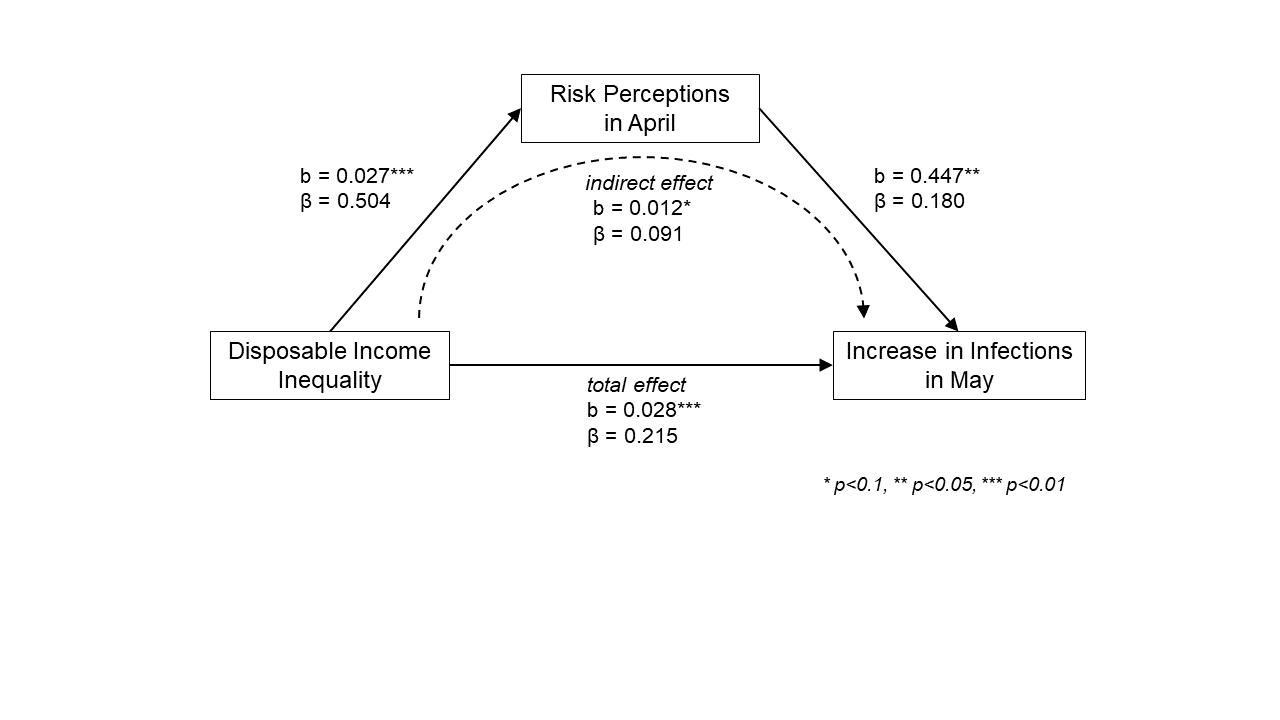
\includegraphics[width=17.78in]{results/Fig4}

\hypertarget{m42}{%
\paragraph{M42}\label{m42}}

This adds the squared term for risk perceptions.

\begin{Shaded}
\begin{Highlighting}[]
\NormalTok{m42 <-}\StringTok{ '   # direct effect}
\StringTok{             rate_2 ~ c1*gini_dispR + c2*gini_disp2 + days_since_peak + conf_delta + gov_resp }
\StringTok{           # mediator}
\StringTok{             concern_self ~ a1*gini_dispR + a2*gini_disp2 + days_since_peak + conf_delta + gov_resp }
\StringTok{             rate_2 ~ b1*concern_self + b2*concern_self2}
\StringTok{           # this is critical because we constructed one out of the other   }
\StringTok{             concern_self2 ~ concern_self}
\StringTok{           # covariances}

\StringTok{           # intercepts}
\StringTok{             rate_2 ~ 1}
\StringTok{             concern_self ~ 1}
\StringTok{           # constraints}
\StringTok{             c2 == 0}
\StringTok{             a2 == 0}

\StringTok{         '}
\NormalTok{m42fit <-}\StringTok{ }\KeywordTok{sem}\NormalTok{(m42, }\DataTypeTok{data =}\NormalTok{ df, }\DataTypeTok{meanstructure =}\NormalTok{ T)}
\KeywordTok{summary}\NormalTok{(m42fit, }\DataTypeTok{fit.measures =}\NormalTok{ T)}
\end{Highlighting}
\end{Shaded}

\begin{verbatim}
## lavaan 0.6-7 ended normally after 107 iterations
## 
##   Estimator                                         ML
##   Optimization method                           NLMINB
##   Number of free parameters                         19
##   Number of equality constraints                     2
##                                                       
##   Number of observations                            74
##                                                       
## Model Test User Model:
##                                                       
##   Test statistic                                 8.340
##   Degrees of freedom                                 7
##   P-value (Chi-square)                           0.304
## 
## Model Test Baseline Model:
## 
##   Test statistic                               741.545
##   Degrees of freedom                                18
##   P-value                                        0.000
## 
## User Model versus Baseline Model:
## 
##   Comparative Fit Index (CFI)                    0.998
##   Tucker-Lewis Index (TLI)                       0.995
## 
## Loglikelihood and Information Criteria:
## 
##   Loglikelihood user model (H0)                -19.696
##   Loglikelihood unrestricted model (H1)        -15.526
##                                                       
##   Akaike (AIC)                                  73.393
##   Bayesian (BIC)                               112.562
##   Sample-size adjusted Bayesian (BIC)           58.988
## 
## Root Mean Square Error of Approximation:
## 
##   RMSEA                                          0.051
##   90 Percent confidence interval - lower         0.000
##   90 Percent confidence interval - upper         0.158
##   P-value RMSEA <= 0.05                          0.427
## 
## Standardized Root Mean Square Residual:
## 
##   SRMR                                           0.007
## 
## Parameter Estimates:
## 
##   Standard errors                             Standard
##   Information                                 Expected
##   Information saturated (h1) model          Structured
## 
## Regressions:
##                    Estimate  Std.Err  z-value  P(>|z|)
##   rate_2 ~                                            
##     gini_dspR (c1)    1.519    1.068    1.422    0.155
##     gini_dsp2 (c2)    0.000                           
##     dys_snc_p        -0.030    0.003   -8.803    0.000
##     conf_delt        -0.144    0.106   -1.355    0.175
##     gov_resp         -0.100    0.056   -1.798    0.072
##   concern_self ~                                      
##     gini_dspR (a1)    2.667    0.541    4.930    0.000
##     gini_dsp2 (a2)    0.000       NA                  
##     dys_snc_p         0.000    0.002    0.239    0.811
##     conf_delt         0.199    0.057    3.470    0.001
##     gov_resp         -0.040    0.032   -1.246    0.213
##   rate_2 ~                                            
##     cncrn_slf (b1)  -10.874    3.273   -3.322    0.001
##     cncrn_sl2 (b2)    1.272    0.367    3.464    0.001
##   concern_self2 ~                                     
##     cncrn_slf         8.900    0.048  186.460    0.000
## 
## Intercepts:
##                    Estimate  Std.Err  z-value  P(>|z|)
##    .rate_2           24.142    7.265    3.323    0.001
##    .concern_self      3.486    0.232   15.028    0.000
##    .concern_self2   -19.670    0.216  -91.217    0.000
## 
## Variances:
##                    Estimate  Std.Err  z-value  P(>|z|)
##    .rate_2            0.215    0.035    6.083    0.000
##    .concern_self      0.073    0.012    6.083    0.000
##    .concern_self2     0.022    0.004    6.083    0.000
## 
## Constraints:
##                                                |Slack|
##     c2 - 0                                       0.000
##     a2 - 0                                       0.000
\end{verbatim}

\begin{Shaded}
\begin{Highlighting}[]
\KeywordTok{standardizedsolution}\NormalTok{(m42fit)}
\end{Highlighting}
\end{Shaded}

\begin{verbatim}
##                lhs op             rhs est.std    se        z pvalue ci.lower
## 1           rate_2  ~      gini_dispR   0.116 0.083    1.398  0.162   -0.047
## 2           rate_2  ~      gini_disp2   0.000 0.000    0.000  1.000   -0.001
## 3           rate_2  ~ days_since_peak  -0.674 0.112   -6.035  0.000   -0.892
## 4           rate_2  ~      conf_delta  -0.097 0.073   -1.334  0.182   -0.239
## 5           rate_2  ~        gov_resp  -0.113 0.064   -1.751  0.080   -0.239
## 6     concern_self  ~      gini_dispR   0.504 0.122    4.139  0.000    0.266
## 7     concern_self  ~      gini_disp2   0.000 0.001    0.000  1.000   -0.002
## 8     concern_self  ~ days_since_peak   0.026 0.455    0.058  0.954   -0.865
## 9     concern_self  ~      conf_delta   0.332 0.105    3.157  0.002    0.126
## 10    concern_self  ~        gov_resp  -0.112 0.091   -1.230  0.219   -0.290
## 11          rate_2  ~    concern_self  -4.396 1.516   -2.899  0.004   -7.368
## 12          rate_2  ~   concern_self2   4.580 1.530    2.993  0.003    1.581
## 13   concern_self2  ~    concern_self   0.999 0.001 1821.250  0.000    0.998
## 14          rate_2 ~1                  27.267 8.951    3.046  0.002    9.722
## 15    concern_self ~1                   9.739 1.988    4.897  0.000    5.841
## 16          rate_2 ~~          rate_2   0.275 0.091    3.016  0.003    0.096
## 17    concern_self ~~    concern_self   0.573 0.204    2.807  0.005    0.173
## 18   concern_self2 ~~   concern_self2   0.002 0.001    1.938  0.053    0.000
## 19      gini_dispR ~~      gini_dispR   1.000 0.000       NA     NA    1.000
## 20      gini_dispR ~~      gini_disp2   0.995 0.000       NA     NA    0.995
## 21      gini_dispR ~~ days_since_peak  -0.508 0.000       NA     NA   -0.508
## 22      gini_dispR ~~      conf_delta   0.155 0.000       NA     NA    0.155
## 23      gini_dispR ~~        gov_resp  -0.080 0.000       NA     NA   -0.080
## 24      gini_disp2 ~~      gini_disp2   1.000 0.000       NA     NA    1.000
## 25      gini_disp2 ~~ days_since_peak  -0.514 0.000       NA     NA   -0.514
## 26      gini_disp2 ~~      conf_delta   0.133 0.000       NA     NA    0.133
## 27      gini_disp2 ~~        gov_resp  -0.081 0.000       NA     NA   -0.081
## 28 days_since_peak ~~ days_since_peak   1.000 0.000       NA     NA    1.000
## 29 days_since_peak ~~      conf_delta  -0.386 0.000       NA     NA   -0.386
## 30 days_since_peak ~~        gov_resp   0.178 0.000       NA     NA    0.178
## 31      conf_delta ~~      conf_delta   1.000 0.000       NA     NA    1.000
## 32      conf_delta ~~        gov_resp  -0.123 0.000       NA     NA   -0.123
## 33        gov_resp ~~        gov_resp   1.000 0.000       NA     NA    1.000
## 34   concern_self2 ~1                  -6.168 1.114   -5.537  0.000   -8.351
## 35      gini_dispR ~1                   5.149 0.000       NA     NA    5.149
## 36      gini_disp2 ~1                   2.577 0.000       NA     NA    2.577
## 37 days_since_peak ~1                   1.586 0.000       NA     NA    1.586
## 38      conf_delta ~1                   0.615 0.000       NA     NA    0.615
## 39        gov_resp ~1                   0.000 0.000       NA     NA    0.000
##    ci.upper
## 1     0.279
## 2     0.001
## 3    -0.455
## 4     0.045
## 5     0.013
## 6     0.743
## 7     0.002
## 8     0.918
## 9     0.538
## 10    0.066
## 11   -1.424
## 12    7.580
## 13    1.000
## 14   44.811
## 15   13.636
## 16    0.453
## 17    0.974
## 18    0.004
## 19    1.000
## 20    0.995
## 21   -0.508
## 22    0.155
## 23   -0.080
## 24    1.000
## 25   -0.514
## 26    0.133
## 27   -0.081
## 28    1.000
## 29   -0.386
## 30    0.178
## 31    1.000
## 32   -0.123
## 33    1.000
## 34   -3.985
## 35    5.149
## 36    2.577
## 37    1.586
## 38    0.615
## 39    0.000
\end{verbatim}

\hypertarget{m43}{%
\paragraph{M43}\label{m43}}

\hypertarget{m43-raw-estimates}{%
\subparagraph{M43 raw estimates}\label{m43-raw-estimates}}

\begin{Shaded}
\begin{Highlighting}[]
\NormalTok{m43 <-}\StringTok{ '   # direct effect}
\StringTok{             rate_2 ~ c1*gini_dispR + c2*gini_disp2 + w11*days_since_peak + w12*conf_delta + w13*gov_resp }
\StringTok{           # mediator}
\StringTok{             concern_self ~ a1*gini_dispR + a2*gini_disp2 + w1*days_since_peak + w2*conf_delta + w3*gov_resp }
\StringTok{             rate_2 ~ b1*concern_self + b2*concern_self2 }
\StringTok{           # this is critical because we constructed one out of the other   }
\StringTok{             concern_self2 ~ concern_self}
\StringTok{           # intercept naming}
\StringTok{             concern_self ~ i1*1}
\StringTok{             rate_2 ~ i2*1}
\StringTok{           # constraint}
\StringTok{             a2 == 0}

\StringTok{         '}
\NormalTok{m43fit <-}\StringTok{ }\KeywordTok{sem}\NormalTok{(m43, }\DataTypeTok{data =}\NormalTok{ df, }\DataTypeTok{meanstructure =}\NormalTok{ T)}

\KeywordTok{summary}\NormalTok{(m43fit, }\DataTypeTok{fit.measures =}\NormalTok{ T)}
\end{Highlighting}
\end{Shaded}

\begin{verbatim}
## lavaan 0.6-7 ended normally after 117 iterations
## 
##   Estimator                                         ML
##   Optimization method                           NLMINB
##   Number of free parameters                         19
##   Number of equality constraints                     1
##                                                       
##   Number of observations                            74
##                                                       
## Model Test User Model:
##                                                       
##   Test statistic                                 5.838
##   Degrees of freedom                                 6
##   P-value (Chi-square)                           0.442
## 
## Model Test Baseline Model:
## 
##   Test statistic                               741.545
##   Degrees of freedom                                18
##   P-value                                        0.000
## 
## User Model versus Baseline Model:
## 
##   Comparative Fit Index (CFI)                    1.000
##   Tucker-Lewis Index (TLI)                       1.001
## 
## Loglikelihood and Information Criteria:
## 
##   Loglikelihood user model (H0)                -18.445
##   Loglikelihood unrestricted model (H1)        -15.526
##                                                       
##   Akaike (AIC)                                  72.890
##   Bayesian (BIC)                               114.364
##   Sample-size adjusted Bayesian (BIC)           57.639
## 
## Root Mean Square Error of Approximation:
## 
##   RMSEA                                          0.000
##   90 Percent confidence interval - lower         0.000
##   90 Percent confidence interval - upper         0.149
##   P-value RMSEA <= 0.05                          0.556
## 
## Standardized Root Mean Square Residual:
## 
##   SRMR                                           0.007
## 
## Parameter Estimates:
## 
##   Standard errors                             Standard
##   Information                                 Expected
##   Information saturated (h1) model          Structured
## 
## Regressions:
##                    Estimate  Std.Err  z-value  P(>|z|)
##   rate_2 ~                                            
##     gin_dspR  (c1)  -12.445    8.643   -1.440    0.150
##     gin_dsp2  (c2)   19.457   12.014    1.620    0.105
##     dys_snc_ (w11)   -0.029    0.003   -8.435    0.000
##     conf_dlt (w12)   -0.104    0.108   -0.960    0.337
##     gov_resp (w13)   -0.101    0.055   -1.836    0.066
##   concern_self ~                                      
##     gin_dspR  (a1)    2.667    0.541    4.930    0.000
##     gin_dsp2  (a2)    0.000       NA                  
##     dys_snc_  (w1)    0.000    0.002    0.239    0.811
##     conf_dlt  (w2)    0.199    0.057    3.470    0.001
##     gov_resp  (w3)   -0.040    0.032   -1.246    0.213
##   rate_2 ~                                            
##     cncrn_sl  (b1)  -10.065    3.218   -3.127    0.002
##     cncrn_s2  (b2)    1.184    0.361    3.280    0.001
##   concern_self2 ~                                     
##     cncrn_sl          8.900    0.048  186.460    0.000
## 
## Intercepts:
##                    Estimate  Std.Err  z-value  P(>|z|)
##    .cncrn_slf (i1)    3.486    0.232   15.028    0.000
##    .rate_2    (i2)   24.651    7.288    3.382    0.001
##    .cncrn_sl2       -19.670    0.216  -91.217    0.000
## 
## Variances:
##                    Estimate  Std.Err  z-value  P(>|z|)
##    .rate_2            0.208    0.034    6.083    0.000
##    .concern_self      0.073    0.012    6.083    0.000
##    .concern_self2     0.022    0.004    6.083    0.000
## 
## Constraints:
##                                                |Slack|
##     a2 - 0                                       0.000
\end{verbatim}

\begin{Shaded}
\begin{Highlighting}[]
\KeywordTok{standardizedsolution}\NormalTok{(m43fit)}
\end{Highlighting}
\end{Shaded}

\begin{verbatim}
##                lhs op             rhs est.std     se        z pvalue ci.lower
## 1           rate_2  ~      gini_dispR  -0.953  0.713   -1.337  0.181   -2.350
## 2           rate_2  ~      gini_disp2   1.076  0.729    1.477  0.140   -0.352
## 3           rate_2  ~ days_since_peak  -0.649  0.192   -3.371  0.001   -1.026
## 4           rate_2  ~      conf_delta  -0.070  0.076   -0.927  0.354   -0.219
## 5           rate_2  ~        gov_resp  -0.113  0.069   -1.637  0.102   -0.249
## 6     concern_self  ~      gini_dispR   0.504  0.180    2.799  0.005    0.151
## 7     concern_self  ~      gini_disp2   0.000  0.002    0.000  1.000   -0.004
## 8     concern_self  ~ days_since_peak   0.026  0.833    0.032  0.975   -1.606
## 9     concern_self  ~      conf_delta   0.332  0.137    2.427  0.015    0.064
## 10    concern_self  ~        gov_resp  -0.112  0.095   -1.171  0.242   -0.299
## 11          rate_2  ~    concern_self  -4.075  1.843   -2.211  0.027   -7.688
## 12          rate_2  ~   concern_self2   4.271  1.884    2.267  0.023    0.578
## 13   concern_self2  ~    concern_self   0.999  0.001 1002.766  0.000    0.997
## 14    concern_self ~1                   9.739  3.244    3.002  0.003    3.380
## 15          rate_2 ~1                  27.883 11.322    2.463  0.014    5.692
## 16          rate_2 ~~          rate_2   0.266  0.158    1.689  0.091   -0.043
## 17    concern_self ~~    concern_self   0.573  0.363    1.577  0.115   -0.139
## 18   concern_self2 ~~   concern_self2   0.002  0.002    1.067  0.286   -0.002
## 19      gini_dispR ~~      gini_dispR   1.000  0.000       NA     NA    1.000
## 20      gini_dispR ~~      gini_disp2   0.995  0.000       NA     NA    0.995
## 21      gini_dispR ~~ days_since_peak  -0.508  0.000       NA     NA   -0.508
## 22      gini_dispR ~~      conf_delta   0.155  0.000       NA     NA    0.155
## 23      gini_dispR ~~        gov_resp  -0.080  0.000       NA     NA   -0.080
## 24      gini_disp2 ~~      gini_disp2   1.000  0.000       NA     NA    1.000
## 25      gini_disp2 ~~ days_since_peak  -0.514  0.000       NA     NA   -0.514
## 26      gini_disp2 ~~      conf_delta   0.133  0.000       NA     NA    0.133
## 27      gini_disp2 ~~        gov_resp  -0.081  0.000       NA     NA   -0.081
## 28 days_since_peak ~~ days_since_peak   1.000  0.000       NA     NA    1.000
## 29 days_since_peak ~~      conf_delta  -0.386  0.000       NA     NA   -0.386
## 30 days_since_peak ~~        gov_resp   0.178  0.000       NA     NA    0.178
## 31      conf_delta ~~      conf_delta   1.000  0.000       NA     NA    1.000
## 32      conf_delta ~~        gov_resp  -0.123  0.000       NA     NA   -0.123
## 33        gov_resp ~~        gov_resp   1.000  0.000       NA     NA    1.000
## 34   concern_self2 ~1                  -6.168  1.966   -3.138  0.002  -10.021
## 35      gini_dispR ~1                   5.149  0.000       NA     NA    5.149
## 36      gini_disp2 ~1                   2.577  0.000       NA     NA    2.577
## 37 days_since_peak ~1                   1.586  0.000       NA     NA    1.586
## 38      conf_delta ~1                   0.615  0.000       NA     NA    0.615
## 39        gov_resp ~1                   0.000  0.000       NA     NA    0.000
##    ci.upper
## 1     0.444
## 2     2.505
## 3    -0.272
## 4     0.078
## 5     0.022
## 6     0.858
## 7     0.004
## 8     1.659
## 9     0.600
## 10    0.075
## 11   -0.463
## 12    7.964
## 13    1.001
## 14   16.098
## 15   50.074
## 16    0.576
## 17    1.286
## 18    0.006
## 19    1.000
## 20    0.995
## 21   -0.508
## 22    0.155
## 23   -0.080
## 24    1.000
## 25   -0.514
## 26    0.133
## 27   -0.081
## 28    1.000
## 29   -0.386
## 30    0.178
## 31    1.000
## 32   -0.123
## 33    1.000
## 34   -2.315
## 35    5.149
## 36    2.577
## 37    1.586
## 38    0.615
## 39    0.000
\end{verbatim}

\hypertarget{m43-for-predictioncalculation}{%
\paragraph{M43 for
prediction/calculation}\label{m43-for-predictioncalculation}}

This strategy follows Hayes and Preacher (2010). The effect is
non-linear meaning that it is heterogeneous. There is no single value of
the income inequality effect. Hayes and Preacher (2010) suggest
estimating an \textbf{instantaneous indirect effect} which is actually
based on derivatives and then can be plotted as different effects at
different levels.

Table 1 in Hayes and Preacher (2010) offers the derivation of the
formulas:

Mediation Formulas

\(\hat{Y} = i_{2} + c'_{1}X + c'_{2}X^{2} + b_{1}M + b_{2}M^{2}\)

\(\hat{M} = i_{1} + aX\)

Instantaneous Indirect Effects of \(X\) on \(Y\) through \(M\) are
derived as (Table 1):

\(a(b_{1} + 2b_{2}\hat{M})\))

The only problem is that the effect of X includes a squared term, this
squared term must be treated as a covariate (like \(W\) in their paper)
and then the model should work, changing the squared term's fixed value
for each.

Also, to get predicted instantaneous indirect effect we need to remove
the covariance of concern\_self and gini\_disp2 from contaminating the
estimates. We fixed gini\_disp2 to zero in the equation for
concern\_self, thus the algorithm find every other possible way to
explain this residual correlation before letting it fall into the
residual. This likely skews the results, therefore, for prediction
purposes we allow all of this correlation to simply fall into the
residual thus alighing the instantaneous indirect effect with the
predicted values of rate\_2

\begin{Shaded}
\begin{Highlighting}[]
\NormalTok{m43p <-}\StringTok{ '   # direct effect}
\StringTok{             rate_2 ~ c1*gini_dispR + c2*gini_disp2 + w11*days_since_peak + w12*conf_delta + w13*gov_resp }
\StringTok{           # mediator}
\StringTok{             concern_self ~ a1*gini_dispR + a2*gini_disp2 + w1*days_since_peak + w2*conf_delta + w3*gov_resp }
\StringTok{             rate_2 ~ b1*concern_self + b2*concern_self2 }
\StringTok{           # this is critical because we constructed one out of the other   }
\StringTok{             concern_self2 ~ concern_self}
\StringTok{           # to fix the residual variance out of the predictions of the model this is necessary}
\StringTok{             concern_self ~~ gini_disp2}
\StringTok{           # intercept naming}
\StringTok{             concern_self ~ i1*1}
\StringTok{             rate_2 ~ i2*1}
\StringTok{           # constraint}
\StringTok{             a2 == 0}
\StringTok{           # instantaneous indir effect calc at values}
\StringTok{             x1 := .225}
\StringTok{             x2 := .25}
\StringTok{             x3 := .275}
\StringTok{             x4 := .30}
\StringTok{             x5 := .325}
\StringTok{             x6 := .35}
\StringTok{             x7 := .375}
\StringTok{             x8 := .40}
\StringTok{             x9 := .425}
\StringTok{             x10 := .45}
\StringTok{             x11 := .475}
\StringTok{             x12 := .50}
\StringTok{           # requires fixing covariates and gini_disp2 = 0 }
\StringTok{             predm1 := i1+(a1*x1)+w1*.30+w2*0.37+0*w3}
\StringTok{             predm2 := i1+(a1*x2)+w1*.30+w2*0.37+0*w3}
\StringTok{             predm3 := i1+(a1*x3)+w1*.30+w2*0.37+0*w3}
\StringTok{             predm4 := i1+(a1*x4)+w1*.30+w2*0.37+0*w3}
\StringTok{             predm5 := i1+(a1*x5)+w1*.30+w2*0.37+0*w3}
\StringTok{             predm6 := i1+(a1*x6)+w1*.30+w2*0.37+0*w3}
\StringTok{             predm7 := i1+(a1*x7)+w1*.30+w2*0.37+0*w3}
\StringTok{             predm8 := i1+(a1*x8)+w1*.30+w2*0.37+0*w3}
\StringTok{             predm9 := i1+(a1*x9)+w1*.30+w2*0.37+0*w3}
\StringTok{             predm10 := i1+(a1*x10)+w1*.30+w2*0.37+0*w3}
\StringTok{             predm11 := i1+(a1*x11)+w1*.30+w2*0.37+0*w3}
\StringTok{             predm12 := i1+(a1*x12)+w1*.30+w2*0.37+0*w3}
\StringTok{           # instantaneous indirect effects (gini_disp2 must be held constant here)}
\StringTok{             theta1 := (b1+2*b2*predm1)*a1}
\StringTok{             theta2 := (b1+2*b2*predm2)*a1}
\StringTok{             theta3 := (b1+2*b2*predm3)*a1}
\StringTok{             theta4 := (b1+2*b2*predm4)*a1}
\StringTok{             theta5 := (b1+2*b2*predm5)*a1}
\StringTok{             theta6 := (b1+2*b2*predm6)*a1}
\StringTok{             theta7 := (b1+2*b2*predm7)*a1}
\StringTok{             theta8 := (b1+2*b2*predm8)*a1}
\StringTok{             theta9 := (b1+2*b2*predm9)*a1}
\StringTok{             theta10 := (b1+2*b2*predm10)*a1}
\StringTok{             theta11 := (b1+2*b2*predm11)*a1}
\StringTok{             theta12 := (b1+2*b2*predm12)*a1}
\StringTok{           # pred values}
\StringTok{             predy1 := i2 + c1*x1 + c2*x1*x1 + b1*predm1 + b2*predm1*predm1 + w11*.30+w12*0.37+0*w13}
\StringTok{             predy2 := i2 + c1*x2 + c2*x2*x2 + b1*predm2 + b2*predm2*predm2 + w11*.30+w12*0.37+0*w13}
\StringTok{             predy3 := i2 + c1*x3 + c2*x3*x3 + b1*predm3 + b2*predm3*predm3 + w11*.30+w12*0.37+0*w13}
\StringTok{             predy4 := i2 + c1*x4 + c2*x4*x4 + b1*predm4 + b2*predm4*predm4 + w11*.30+w12*0.37+0*w13}
\StringTok{             predy5 := i2 + c1*x5 + c2*x5*x5 + b1*predm5 + b2*predm5*predm5 + w11*.30+w12*0.37+0*w13}
\StringTok{             predy6 := i2 + c1*x6 + c2*x6*x6 + b1*predm6 + b2*predm6*predm6 + w11*.30+w12*0.37+0*w13}
\StringTok{             predy7 := i2 + c1*x7 + c2*x7*x7 + b1*predm7 + b2*predm7*predm7 + w11*.30+w12*0.37+0*w13}
\StringTok{             predy8 := i2 + c1*x8 + c2*x8*x8 + b1*predm8 + b2*predm8*predm8 + w11*.30+w12*0.37+0*w13}
\StringTok{             predy9 := i2 + c1*x9 + c2*x9*x9 + b1*predm9 + b2*predm9*predm9 + w11*.30+w12*0.37+0*w13}
\StringTok{             predy10 := i2 + c1*x10 + c2*x10*x10 + b1*predm10 + b2*predm10*predm10 + w11*.30+w12*0.37+0*w13}
\StringTok{             predy11 := i2 + c1*x11 + c2*x11*x11 + b1*predm11 + b2*predm11*predm11 + w11*.30+w12*0.37+0*w13}
\StringTok{             predy12 := i2 + c1*x12 + c2*x12*x12 + b1*predm12 + b2*predm12*predm12 + w11*.30+w12*0.37+0*w13}

\StringTok{         '}
\NormalTok{m43pfit <-}\StringTok{ }\KeywordTok{sem}\NormalTok{(m43p, }\DataTypeTok{data =}\NormalTok{ df, }\DataTypeTok{meanstructure =}\NormalTok{ T)}
\end{Highlighting}
\end{Shaded}

\hypertarget{table-2.-main-models}{%
\paragraph{Table 2. Main Models}\label{table-2.-main-models}}

We used an html template from tab\_model command and hand edited the
values to produce a table that was visually identical to Table 1.
Automation would be ideal here, but we double checked the scores.

\begin{Shaded}
\begin{Highlighting}[]
\CommentTok{# set up frames}

\NormalTok{m40tab <-}\StringTok{ }\KeywordTok{matrix}\NormalTok{(}\KeywordTok{summary}\NormalTok{(m40fit, }\DataTypeTok{fit.measures =}\NormalTok{ T))}
\NormalTok{m40fits <-}\StringTok{ }\KeywordTok{as.data.frame}\NormalTok{(m40tab[[}\DecValTok{1}\NormalTok{]])}
\NormalTok{m40parm <-}\StringTok{ }\KeywordTok{as.data.frame}\NormalTok{(m40tab[[}\DecValTok{2}\NormalTok{]])}
\NormalTok{m40parm <-}\StringTok{ }\KeywordTok{select}\NormalTok{(m40parm, }\OperatorTok{-}\KeywordTok{c}\NormalTok{(label, exo))}
\NormalTok{m41tab <-}\StringTok{ }\KeywordTok{matrix}\NormalTok{(}\KeywordTok{summary}\NormalTok{(m41fit, }\DataTypeTok{fit.measures =}\NormalTok{ T))}
\NormalTok{m41fits <-}\StringTok{ }\KeywordTok{as.data.frame}\NormalTok{(m41tab[[}\DecValTok{1}\NormalTok{]])}
\NormalTok{m41parm <-}\StringTok{ }\KeywordTok{as.data.frame}\NormalTok{(m41tab[[}\DecValTok{2}\NormalTok{]])}
\NormalTok{m41parm <-}\StringTok{ }\KeywordTok{select}\NormalTok{(m41parm, }\OperatorTok{-}\KeywordTok{c}\NormalTok{(label, exo))}
\NormalTok{m42tab <-}\StringTok{ }\KeywordTok{matrix}\NormalTok{(}\KeywordTok{summary}\NormalTok{(m42fit, }\DataTypeTok{fit.measures =}\NormalTok{ T))}
\NormalTok{m42fits <-}\StringTok{ }\KeywordTok{as.data.frame}\NormalTok{(m42tab[[}\DecValTok{1}\NormalTok{]])}
\NormalTok{m42parm <-}\StringTok{ }\KeywordTok{as.data.frame}\NormalTok{(m42tab[[}\DecValTok{2}\NormalTok{]])}
\NormalTok{m42parm <-}\StringTok{ }\KeywordTok{select}\NormalTok{(m42parm, }\OperatorTok{-}\KeywordTok{c}\NormalTok{(label,exo))}
\NormalTok{m43tab <-}\StringTok{ }\KeywordTok{matrix}\NormalTok{(}\KeywordTok{summary}\NormalTok{(m43fit, }\DataTypeTok{fit.measures =}\NormalTok{ T))}
\NormalTok{m43fits <-}\StringTok{ }\KeywordTok{as.data.frame}\NormalTok{(m43tab[[}\DecValTok{1}\NormalTok{]])}
\NormalTok{m43parm <-}\StringTok{ }\KeywordTok{as.data.frame}\NormalTok{(m43tab[[}\DecValTok{2}\NormalTok{]])}
\NormalTok{m43parm <-}\StringTok{ }\KeywordTok{select}\NormalTok{(m43parm, }\OperatorTok{-}\KeywordTok{c}\NormalTok{(label, exo))}

\CommentTok{# combine and name which results go with which models}

\NormalTok{semtab <-}\StringTok{ }\KeywordTok{rbind}\NormalTok{(m40parm,m41parm,m42parm,m43parm)}
\NormalTok{semtab_labels <-}\StringTok{ }\KeywordTok{as.data.frame}\NormalTok{(}\KeywordTok{matrix}\NormalTok{(}\DataTypeTok{nrow =} \KeywordTok{length}\NormalTok{(semtab[,}\DecValTok{1}\NormalTok{]), }\DataTypeTok{ncol =} \DecValTok{1}\NormalTok{))}
\NormalTok{semtab_labels}\OperatorTok{$}\NormalTok{V1 <-}\StringTok{ }\KeywordTok{as.list}\NormalTok{(}\KeywordTok{unlist}\NormalTok{(}\KeywordTok{strsplit}\NormalTok{(}\KeywordTok{paste}\NormalTok{(}\KeywordTok{paste}\NormalTok{(}\KeywordTok{replicate}\NormalTok{(}\KeywordTok{length}\NormalTok{(m40parm[,}\DecValTok{1}\NormalTok{]), }\StringTok{"m40"}\NormalTok{), }\DataTypeTok{collapse =} \StringTok{","}\NormalTok{), }\KeywordTok{paste}\NormalTok{(}\KeywordTok{replicate}\NormalTok{(}\KeywordTok{length}\NormalTok{(m41parm[,}\DecValTok{1}\NormalTok{]), }\StringTok{"m41"}\NormalTok{), }\DataTypeTok{collapse =} \StringTok{","}\NormalTok{), }\KeywordTok{paste}\NormalTok{(}\KeywordTok{replicate}\NormalTok{(}\KeywordTok{length}\NormalTok{(m42parm[,}\DecValTok{1}\NormalTok{]), }\StringTok{"m42"}\NormalTok{), }\DataTypeTok{collapse =} \StringTok{","}\NormalTok{), }\KeywordTok{paste}\NormalTok{(}\KeywordTok{replicate}\NormalTok{(}\KeywordTok{length}\NormalTok{(m43parm[,}\DecValTok{1}\NormalTok{]), }\StringTok{"m43"}\NormalTok{), }\DataTypeTok{collapse =} \StringTok{","}\NormalTok{), }\DataTypeTok{sep =} \StringTok{","}\NormalTok{), }\StringTok{","}\NormalTok{)))}

\NormalTok{semtab <-}\StringTok{ }\KeywordTok{cbind}\NormalTok{(semtab_labels, semtab)}
\NormalTok{semtab <-}\StringTok{ }\NormalTok{semtab }\OperatorTok
\StringTok{  }\KeywordTok{mutate}\NormalTok{(}\DataTypeTok{est =} \KeywordTok{round}\NormalTok{(est,}\DecValTok{3}\NormalTok{),}
         \DataTypeTok{se =} \KeywordTok{round}\NormalTok{(se,}\DecValTok{3}\NormalTok{),}
         \DataTypeTok{pvalue =} \KeywordTok{round}\NormalTok{(pvalue,}\DecValTok{3}\NormalTok{),}
         \DataTypeTok{stars =} \KeywordTok{ifelse}\NormalTok{(pvalue}\OperatorTok{>}\FloatTok{0.1}\NormalTok{,}\StringTok{""}\NormalTok{, }\KeywordTok{ifelse}\NormalTok{(pvalue}\OperatorTok{>}\FloatTok{0.05}\NormalTok{,}\StringTok{"*"}\NormalTok{, }\KeywordTok{ifelse}\NormalTok{(pvalue}\OperatorTok{>}\FloatTok{0.01}\NormalTok{,}\StringTok{"**"}\NormalTok{,}\StringTok{"***"}\NormalTok{))),}
         \DataTypeTok{est =} \KeywordTok{ifelse}\NormalTok{(rhs }\OperatorTok{==}\StringTok{ "gini_dispR"} \OperatorTok{|}\StringTok{ }\NormalTok{rhs }\OperatorTok{==}\StringTok{ "gini_disp2"}\NormalTok{, est}\OperatorTok{/}\DecValTok{100}\NormalTok{, est),}
         \DataTypeTok{se =} \KeywordTok{ifelse}\NormalTok{(rhs }\OperatorTok{==}\StringTok{ "gini_dispR"} \OperatorTok{|}\StringTok{ }\NormalTok{rhs }\OperatorTok{==}\StringTok{ "gini_disp2"}\NormalTok{, se}\OperatorTok{/}\DecValTok{100}\NormalTok{, se)}
\NormalTok{  )}

\NormalTok{semtab <-}\StringTok{ }\KeywordTok{subset}\NormalTok{(semtab, op }\OperatorTok{==}\StringTok{ "~"} \OperatorTok{&}\StringTok{ }\NormalTok{lhs}\OperatorTok{!=}\StringTok{ "concern_self2"}\NormalTok{)}


\NormalTok{semfits <-}\StringTok{ }\KeywordTok{round}\NormalTok{(}\KeywordTok{cbind}\NormalTok{(m40fits,m41fits,m42fits,m43fits),}\DecValTok{3}\NormalTok{)}
\KeywordTok{colnames}\NormalTok{(semfits) <-}\StringTok{ }\KeywordTok{c}\NormalTok{(}\StringTok{"m40"}\NormalTok{,}\StringTok{"m41"}\NormalTok{,}\StringTok{"m42"}\NormalTok{,}\StringTok{"m43"}\NormalTok{)}

\CommentTok{# get r-squared}
\NormalTok{m40r2 <-}\StringTok{ }\KeywordTok{round}\NormalTok{(}\KeywordTok{as.data.frame}\NormalTok{(}\KeywordTok{inspect}\NormalTok{(m40fit,}\StringTok{'r2'}\NormalTok{)),}\DecValTok{3}\NormalTok{)}
\NormalTok{m41r2 <-}\StringTok{ }\KeywordTok{round}\NormalTok{(}\KeywordTok{as.data.frame}\NormalTok{(}\KeywordTok{inspect}\NormalTok{(m41fit,}\StringTok{'r2'}\NormalTok{)),}\DecValTok{3}\NormalTok{)}
\NormalTok{m42r2 <-}\StringTok{ }\KeywordTok{round}\NormalTok{(}\KeywordTok{as.data.frame}\NormalTok{(}\KeywordTok{inspect}\NormalTok{(m42fit,}\StringTok{'r2'}\NormalTok{)),}\DecValTok{3}\NormalTok{)}
\NormalTok{m43r2 <-}\StringTok{ }\KeywordTok{round}\NormalTok{(}\KeywordTok{as.data.frame}\NormalTok{(}\KeywordTok{inspect}\NormalTok{(m43fit,}\StringTok{'r2'}\NormalTok{)),}\DecValTok{3}\NormalTok{)}

\NormalTok{semr2s <-}\StringTok{ }\KeywordTok{cbind}\NormalTok{(m40r2,m41r2,m42r2,m43r2)}
\NormalTok{semr2s <-}\StringTok{ }\NormalTok{semr2s[}\DecValTok{1}\OperatorTok{:}\DecValTok{2}\NormalTok{,]}
\KeywordTok{colnames}\NormalTok{(semr2s) <-}\StringTok{ }\KeywordTok{c}\NormalTok{(}\StringTok{"m40"}\NormalTok{,}\StringTok{"m41"}\NormalTok{,}\StringTok{"m42"}\NormalTok{,}\StringTok{"m43"}\NormalTok{)}

\NormalTok{semfits <-}\StringTok{ }\KeywordTok{rbind}\NormalTok{(semfits,semr2s)}

\NormalTok{semfits <-}\StringTok{ }\NormalTok{semfits[}\KeywordTok{c}\NormalTok{(}\StringTok{"rate_2"}\NormalTok{, }\StringTok{"concern_self"}\NormalTok{, }\StringTok{"aic"}\NormalTok{, }\StringTok{"bic"}\NormalTok{, }\StringTok{"logl"}\NormalTok{),]}

\KeywordTok{rm}\NormalTok{(m40tab, m40fits, m40parm, m41tab, m41fits, m41parm, m42tab, m42fits, m42parm, m43tab, m43fits, m43parm, m40r2,m41r2,m42r2,m43r2, semr2s, semtab_labels)}

\KeywordTok{kable}\NormalTok{(semtab)}
\KeywordTok{kable}\NormalTok{(semfits)}
\end{Highlighting}
\end{Shaded}

To create a table identical to the tab\_model table we adjust the html
code by hand, but hopefully we can automate this in the future.

\begin{Shaded}
\begin{Highlighting}[]
\NormalTok{knitr}\OperatorTok{::}\KeywordTok{include_graphics}\NormalTok{(}\StringTok{"results/Tbl2.png"}\NormalTok{)}
\end{Highlighting}
\end{Shaded}

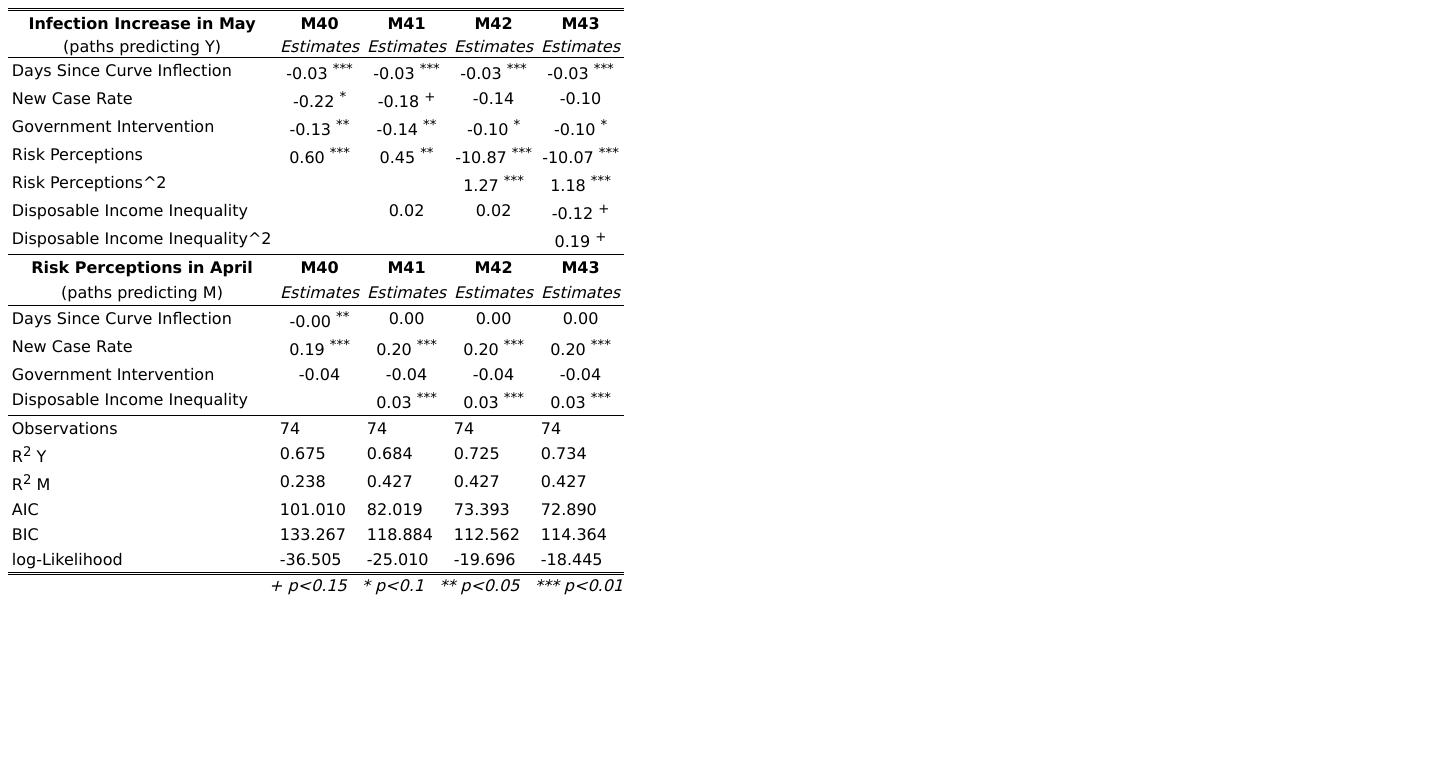
\includegraphics[width=20in]{results/Tbl2}

\hypertarget{figure-5}{%
\paragraph{Figure 5}\label{figure-5}}

\begin{Shaded}
\begin{Highlighting}[]
\NormalTok{m43mat <-}\StringTok{ }\KeywordTok{summary}\NormalTok{(m43pfit)}
\NormalTok{m43mat <-}\StringTok{ }\KeywordTok{as.data.frame}\NormalTok{(m43mat[[}\StringTok{"PE"}\NormalTok{]])}
\NormalTok{a43 <-}\StringTok{ }\NormalTok{m43mat[}\DecValTok{38}\OperatorTok{:}\DecValTok{49}\NormalTok{,]}
\NormalTok{a43 <-}\StringTok{ }\KeywordTok{select}\NormalTok{(a43, rhs)}
\NormalTok{a43}\OperatorTok{$}\NormalTok{rhs <-}\StringTok{ }\KeywordTok{as.numeric}\NormalTok{(a43}\OperatorTok{$}\NormalTok{rhs)}
\KeywordTok{colnames}\NormalTok{(a43) <-}\StringTok{ }\KeywordTok{c}\NormalTok{(}\StringTok{"X_gini"}\NormalTok{)}
\NormalTok{b43 <-}\StringTok{ }\NormalTok{m43mat[}\DecValTok{50}\OperatorTok{:}\DecValTok{61}\NormalTok{,]}
\NormalTok{b43 <-}\StringTok{ }\KeywordTok{select}\NormalTok{(b43, label, est)}
\KeywordTok{colnames}\NormalTok{(b43) <-}\StringTok{ }\KeywordTok{c}\NormalTok{(}\StringTok{"moderator"}\NormalTok{,}\StringTok{"pred_M"}\NormalTok{)}
\NormalTok{c43 <-}\StringTok{ }\NormalTok{m43mat[}\DecValTok{62}\OperatorTok{:}\DecValTok{73}\NormalTok{,]}
\NormalTok{c43 <-}\StringTok{ }\KeywordTok{select}\NormalTok{(c43, est, se, z, pvalue)}
\KeywordTok{colnames}\NormalTok{(c43) <-}\StringTok{ }\KeywordTok{c}\NormalTok{(}\StringTok{"inst_indr_effect"}\NormalTok{,}\StringTok{"iie_se"}\NormalTok{,}\StringTok{"iie_z"}\NormalTok{,}\StringTok{"iie_p"}\NormalTok{)}
\NormalTok{d43 <-}\StringTok{ }\NormalTok{m43mat[}\DecValTok{74}\OperatorTok{:}\DecValTok{85}\NormalTok{,]}
\NormalTok{d43 <-}\StringTok{ }\KeywordTok{select}\NormalTok{(d43, est, se, z, pvalue)}
\KeywordTok{colnames}\NormalTok{(d43) <-}\StringTok{ }\KeywordTok{c}\NormalTok{(}\StringTok{"pred_Y"}\NormalTok{,}\StringTok{"Y_se"}\NormalTok{,}\StringTok{"Y_z"}\NormalTok{,}\StringTok{"Y_p"}\NormalTok{)}

\NormalTok{m43mat <-}\StringTok{ }\KeywordTok{cbind}\NormalTok{(a43,b43,c43,d43)}

\CommentTok{# Now transform so that all values are relative to an 'average', axis cross}

\CommentTok{# 1 - rescale Gini back into its 100-point original scale}
\NormalTok{m43mat <-}\StringTok{ }\NormalTok{m43mat }\OperatorTok
\StringTok{  }\KeywordTok{mutate}\NormalTok{(}\DataTypeTok{X_gini =} \KeywordTok{round}\NormalTok{(X_gini}\OperatorTok{*}\DecValTok{100}\NormalTok{,}\DecValTok{1}\NormalTok{),}
         \DataTypeTok{pred_MC =}\NormalTok{ pred_M }\OperatorTok{-}\StringTok{ }\KeywordTok{mean}\NormalTok{(pred_M),}
         \DataTypeTok{iie_orig =}\NormalTok{ inst_indr_effect}\OperatorTok{/}\DecValTok{100}\NormalTok{,}
         \DataTypeTok{iie_origC =}\NormalTok{ iie_orig }\OperatorTok{-}\StringTok{ }\KeywordTok{mean}\NormalTok{(iie_orig),}
         \DataTypeTok{pred_YavgC =} \FloatTok{0.33820}\OperatorTok{*}\NormalTok{pred_Y, }\CommentTok{# make avg-Y_hat mean = avg-Y mean}
         \DataTypeTok{ymin =}\NormalTok{ pred_YavgC }\OperatorTok{-}\StringTok{ }\FloatTok{1.96}\OperatorTok{*}\NormalTok{Y_se}\OperatorTok{*}\FloatTok{0.33820}\NormalTok{,}
         \DataTypeTok{ymax =}\NormalTok{ pred_YavgC }\OperatorTok{+}\StringTok{ }\FloatTok{1.96}\OperatorTok{*}\NormalTok{Y_se}\OperatorTok{*}\FloatTok{0.33820}\NormalTok{)}\CommentTok{# add 95% confidence intervals)}



\KeywordTok{rm}\NormalTok{(a43,b43,c43,d43)}
\end{Highlighting}
\end{Shaded}

\begin{Shaded}
\begin{Highlighting}[]
\KeywordTok{agg_png}\NormalTok{(}\DataTypeTok{file =} \StringTok{"results/Fig5.png"}\NormalTok{, }\DataTypeTok{width =} \DecValTok{800}\NormalTok{, }\DataTypeTok{height =} \DecValTok{600}\NormalTok{, }\DataTypeTok{res =} \DecValTok{144}\NormalTok{)}
\KeywordTok{ggplot}\NormalTok{(}\DataTypeTok{data =}\NormalTok{ m43mat, }\KeywordTok{aes}\NormalTok{(}\DataTypeTok{x =}\NormalTok{ X_gini)) }\OperatorTok{+}
\StringTok{  }\KeywordTok{geom_abline}\NormalTok{(}\DataTypeTok{intercept =} \DecValTok{0}\NormalTok{, }\DataTypeTok{slope =} \DecValTok{0}\NormalTok{, }\DataTypeTok{size =} \FloatTok{0.25}\NormalTok{, }\DataTypeTok{color =} \StringTok{"grey2"}\NormalTok{) }\OperatorTok{+}
\StringTok{  }\KeywordTok{geom_ribbon}\NormalTok{(}\KeywordTok{aes}\NormalTok{(}\DataTypeTok{ymin=}\NormalTok{ymin,}\DataTypeTok{ymax=}\NormalTok{ymax), }\DataTypeTok{fill =} \StringTok{"grey70"}\NormalTok{) }\OperatorTok{+}
\StringTok{  }\KeywordTok{geom_line}\NormalTok{(}\KeywordTok{aes}\NormalTok{(}\DataTypeTok{y =}\NormalTok{ pred_YavgC, }\DataTypeTok{color =} \StringTok{"a"}\NormalTok{), }\DataTypeTok{size =} \DecValTok{1}\NormalTok{) }\OperatorTok{+}
\StringTok{  }\KeywordTok{geom_line}\NormalTok{(}\KeywordTok{aes}\NormalTok{(}\DataTypeTok{y =}\NormalTok{ pred_MC, }\DataTypeTok{color =} \StringTok{"b"}\NormalTok{), }\DataTypeTok{size =} \DecValTok{1}\NormalTok{) }\OperatorTok{+}
\StringTok{  }\KeywordTok{geom_line}\NormalTok{(}\KeywordTok{aes}\NormalTok{(}\DataTypeTok{y =}\NormalTok{ iie_orig, }\DataTypeTok{color =} \StringTok{"c"}\NormalTok{), }\DataTypeTok{size =} \DecValTok{1}\NormalTok{) }\OperatorTok{+}
\StringTok{  }\KeywordTok{geom_vline}\NormalTok{(}\DataTypeTok{xintercept =} \DecValTok{31}\NormalTok{, }\DataTypeTok{linetype =} \DecValTok{5}\NormalTok{, }\DataTypeTok{color =} \StringTok{"darkgoldenrod4"}\NormalTok{) }\OperatorTok{+}
\StringTok{  }\KeywordTok{annotate}\NormalTok{(}\DataTypeTok{geom=}\StringTok{"label"}\NormalTok{, }\DataTypeTok{x=}\DecValTok{26}\NormalTok{, }\DataTypeTok{y=}\FloatTok{1.7}\NormalTok{, }\DataTypeTok{label=}\StringTok{"Increasing inequality =}\CharTok{\textbackslash{}n}\StringTok{LESS infections"}\NormalTok{,}
              \DataTypeTok{color=}\StringTok{"darkgoldenrod4"}\NormalTok{, }\DataTypeTok{size =} \FloatTok{2.5}\NormalTok{) }\OperatorTok{+}
\StringTok{  }\KeywordTok{annotate}\NormalTok{(}\DataTypeTok{geom=}\StringTok{"label"}\NormalTok{, }\DataTypeTok{x=}\DecValTok{36}\NormalTok{, }\DataTypeTok{y=}\FloatTok{1.7}\NormalTok{, }\DataTypeTok{label=}\StringTok{"Increasing inequality =}\CharTok{\textbackslash{}n}\StringTok{MORE infections"}\NormalTok{,}
              \DataTypeTok{color=}\StringTok{"darkgoldenrod4"}\NormalTok{, }\DataTypeTok{size =} \FloatTok{2.5}\NormalTok{) }\OperatorTok{+}
\StringTok{  }\KeywordTok{geom_segment}\NormalTok{(}\KeywordTok{aes}\NormalTok{(}\DataTypeTok{x =} \FloatTok{30.5}\NormalTok{, }\DataTypeTok{y =} \FloatTok{1.7}\NormalTok{, }\DataTypeTok{xend =} \FloatTok{29.5}\NormalTok{, }\DataTypeTok{yend =} \FloatTok{1.7}\NormalTok{),}
                  \DataTypeTok{arrow =} \KeywordTok{arrow}\NormalTok{(}\DataTypeTok{length =} \KeywordTok{unit}\NormalTok{(}\FloatTok{0.2}\NormalTok{, }\StringTok{"cm"}\NormalTok{), }\DataTypeTok{type =} \StringTok{"closed"}\NormalTok{), }\DataTypeTok{colour =} \StringTok{"darkgoldenrod4"}\NormalTok{) }\OperatorTok{+}
\StringTok{  }\KeywordTok{geom_segment}\NormalTok{(}\KeywordTok{aes}\NormalTok{(}\DataTypeTok{x =} \FloatTok{31.5}\NormalTok{, }\DataTypeTok{y =} \FloatTok{1.7}\NormalTok{, }\DataTypeTok{xend =} \FloatTok{32.5}\NormalTok{, }\DataTypeTok{yend =} \FloatTok{1.7}\NormalTok{),}
                  \DataTypeTok{arrow =} \KeywordTok{arrow}\NormalTok{(}\DataTypeTok{length =} \KeywordTok{unit}\NormalTok{(}\FloatTok{0.2}\NormalTok{, }\StringTok{"cm"}\NormalTok{), }\DataTypeTok{type =} \StringTok{"closed"}\NormalTok{), }\DataTypeTok{colour =} \StringTok{"darkgoldenrod4"}\NormalTok{) }\OperatorTok{+}
\StringTok{  }\KeywordTok{scale_color_manual}\NormalTok{(}\DataTypeTok{name =} \StringTok{""}\NormalTok{, }\DataTypeTok{labels =} \KeywordTok{c}\NormalTok{(}\StringTok{"a"}\NormalTok{ =}\StringTok{ "Infection Increase (Y)}\CharTok{\textbackslash{}n}\StringTok{May 1st to May 31st}\CharTok{\textbackslash{}n}\StringTok{ratio, predicted"}\NormalTok{, }\StringTok{"c"}\NormalTok{ =}\StringTok{ "Instantaneous}\CharTok{\textbackslash{}n}\StringTok{Indirect Effect}\CharTok{\textbackslash{}n}\StringTok{(rate of change)"}\NormalTok{ , }\StringTok{"b"}\NormalTok{ =}\StringTok{ "Risk Perceptions (M)}\CharTok{\textbackslash{}n}\StringTok{April, 2020}\CharTok{\textbackslash{}n}\StringTok{predicted, centered"}\NormalTok{), }\DataTypeTok{values =} \KeywordTok{c}\NormalTok{(}\StringTok{"a"}\NormalTok{ =}\StringTok{ "red"}\NormalTok{, }\StringTok{"b"}\NormalTok{ =}\StringTok{ "blue"}\NormalTok{, }\StringTok{"c"}\NormalTok{ =}\StringTok{ "darkgoldenrod4"}\NormalTok{)) }\OperatorTok{+}
\StringTok{  }\KeywordTok{scale_x_continuous}\NormalTok{(}\DataTypeTok{breaks =} \KeywordTok{c}\NormalTok{(}\DecValTok{25}\NormalTok{,}\DecValTok{30}\NormalTok{,}\DecValTok{35}\NormalTok{,}\DecValTok{40}\NormalTok{,}\DecValTok{45}\NormalTok{,}\DecValTok{50}\NormalTok{), }\DataTypeTok{expand =} \KeywordTok{c}\NormalTok{(}\DecValTok{0}\NormalTok{,}\DecValTok{0}\NormalTok{)) }\OperatorTok{+}
\StringTok{  }\KeywordTok{scale_y_continuous}\NormalTok{(}\DataTypeTok{breaks =} \KeywordTok{c}\NormalTok{(}\OperatorTok{-}\DecValTok{1}\NormalTok{,}\OperatorTok{-}\FloatTok{0.5}\NormalTok{,}\DecValTok{0}\NormalTok{,}\FloatTok{0.5}\NormalTok{,}\DecValTok{1}\NormalTok{,}\FloatTok{1.5}\NormalTok{,}\DecValTok{2}\NormalTok{), }\DataTypeTok{limits =} \KeywordTok{c}\NormalTok{(}\OperatorTok{-}\DecValTok{1}\NormalTok{,}\DecValTok{2}\NormalTok{), }\DataTypeTok{expand =} \KeywordTok{c}\NormalTok{(}\DecValTok{0}\NormalTok{,}\DecValTok{0}\NormalTok{)) }\OperatorTok{+}
\StringTok{  }\KeywordTok{labs}\NormalTok{(}\DataTypeTok{x =} \StringTok{"Disposable Income Inequality (X), gini"}\NormalTok{,}\DataTypeTok{y =} \StringTok{"Estimate"}\NormalTok{) }\OperatorTok{+}
\StringTok{  }\KeywordTok{theme}\NormalTok{(}\DataTypeTok{panel.background =} \KeywordTok{element_blank}\NormalTok{(),}
        \DataTypeTok{panel.grid =} \KeywordTok{element_blank}\NormalTok{(),}
        \DataTypeTok{axis.line =} \KeywordTok{element_line}\NormalTok{(),}
        \DataTypeTok{legend.position =} \StringTok{"bottom"}\NormalTok{,}
        \DataTypeTok{legend.background =} \KeywordTok{element_rect}\NormalTok{(}\DataTypeTok{fill =} \StringTok{"#BFD5E3"}\NormalTok{),}
        \DataTypeTok{legend.key =} \KeywordTok{element_rect}\NormalTok{(}\DataTypeTok{fill =} \StringTok{"#BFD5E3"}\NormalTok{),}
        \DataTypeTok{plot.margin=}\KeywordTok{unit}\NormalTok{(}\KeywordTok{c}\NormalTok{(}\DecValTok{1}\NormalTok{,}\DecValTok{1}\NormalTok{,}\FloatTok{0.1}\NormalTok{,}\FloatTok{0.3}\NormalTok{),}\StringTok{"cm"}\NormalTok{))}
\KeywordTok{dev.off}\NormalTok{()}
\end{Highlighting}
\end{Shaded}

\begin{verbatim}
## pdf 
##   2
\end{verbatim}

\begin{Shaded}
\begin{Highlighting}[]
\NormalTok{knitr}\OperatorTok{::}\KeywordTok{include_graphics}\NormalTok{(}\StringTok{"results/Fig5.png"}\NormalTok{)}
\end{Highlighting}
\end{Shaded}

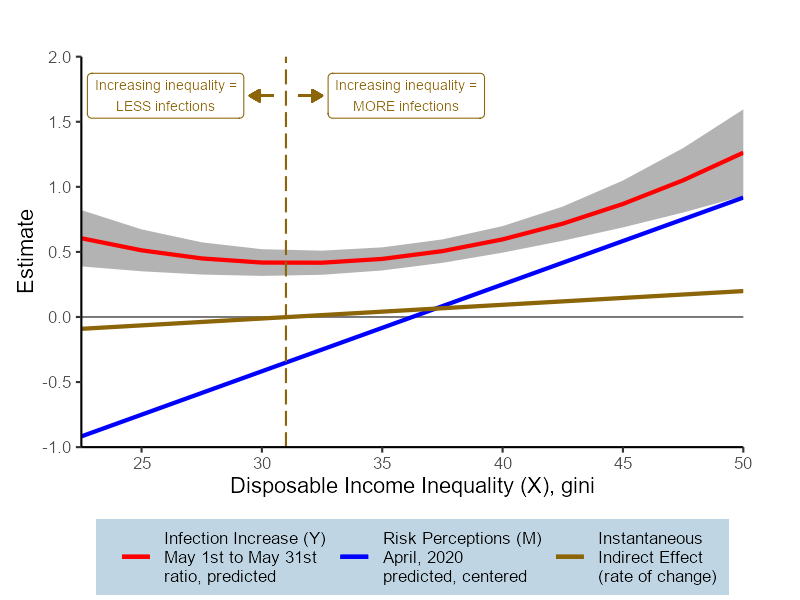
\includegraphics[width=11.11in]{results/Fig5}

We know that there is a risk of random sampling variation causing
disturbance to the results. Therefore we again simulate the variability
in the mean risk perceptions by country.

Get rid of earlier sampling robustness exercise and just do it here for
both.

\hypertarget{robustness-of-mediation-effect-to-sampling.-simulating-plausible-alternative-values-for-country-means}{%
\paragraph{Robustness of Mediation Effect to Sampling. Simulating
Plausible Alternative Values for
Country-Means}\label{robustness-of-mediation-effect-to-sampling.-simulating-plausible-alternative-values-for-country-means}}

The confidence interval of our regression estimates is based on a
sampling distribution across countries, but we have a potentially large
source of uncertainty within countries due to the use of an online
survey and some very small samples. The online survey problem cannot be
solved directly through bootstrapping, but we can asses the robustness
of our estimates using the within-country uncertainty.

We `bootstrap' the estimates by generating random data that follow a
normal distribution for each country based on the standard error. Then
we run the analysis on each dataset to generate a confidence interval
for our estimates that incorporates the within-country standard error of
the mean.

Designate the model and calculate the slope of the indirect effect

\begin{Shaded}
\begin{Highlighting}[]
\NormalTok{r43 <-}\StringTok{ '    rate_2 ~ c1*gini_dispR + c2*gini_disp2 + w11*days_since_peak + w12*conf_delta + w13*gov_resp}
\StringTok{             concern_self ~ a1*gini_dispR + a2*gini_disp2 + w1*days_since_peak + w2*conf_delta + w3*gov_resp }
\StringTok{             rate_2 ~ b1*concern_self + b2*concern_selfsq }
\StringTok{             concern_selfsq ~ concern_self}
\StringTok{             concern_self ~~ gini_disp2}
\StringTok{             concern_self ~ i1*1}
\StringTok{             rate_2 ~ i2*1}
\StringTok{             a2 == 0}
\StringTok{             x1 := .225}
\StringTok{             x12 := .50}
\StringTok{             predm1 := i1+(a1*x1)+w1*.30+w2*0.37+0*w3}
\StringTok{             predm12 := i1+(a1*x12)+w1*.30+w2*0.37+0*w3}
\StringTok{             theta1 := (b1+2*b2*predm1)*a1}
\StringTok{             theta12 := (b1+2*b2*predm12)*a1}
\StringTok{             slope := (theta12-theta1)/(x12-x1)}
\StringTok{             yint := theta12 - (slope*x12)}
\StringTok{             xint := -yint/slope}
\StringTok{         '}
\end{Highlighting}
\end{Shaded}

note with limited RAM I can only do 750 at a time

first 750

\begin{Shaded}
\begin{Highlighting}[]
\CommentTok{# }
\ControlFlowTok{for}\NormalTok{ (i }\ControlFlowTok{in} \DecValTok{1}\OperatorTok{:}\DecValTok{750}\NormalTok{) \{}
  \KeywordTok{assign}\NormalTok{(}\KeywordTok{paste0}\NormalTok{(}\StringTok{"r43_"}\NormalTok{,i), }\KeywordTok{str_replace_all}\NormalTok{(r43, }\StringTok{"concern_self"}\NormalTok{, test[i]))}
\NormalTok{\}}

\CommentTok{# fit first 750 models}

\CommentTok{# get list}
\NormalTok{model.list <-}\StringTok{ }\KeywordTok{mget}\NormalTok{(}\KeywordTok{grep}\NormalTok{(}\StringTok{"r43_[0-9]+$"}\NormalTok{, }\KeywordTok{ls}\NormalTok{(),}\DataTypeTok{value=}\NormalTok{T))}

\CommentTok{# remove values (clear up RAM)}
\KeywordTok{rm}\NormalTok{(}\DataTypeTok{list =} \KeywordTok{ls}\NormalTok{(}\DataTypeTok{pattern =} \StringTok{"r43_"}\NormalTok{))}

\CommentTok{# fitting loop}
\ControlFlowTok{for}\NormalTok{ (m }\ControlFlowTok{in} \DecValTok{1}\OperatorTok{:}\KeywordTok{length}\NormalTok{(model.list)) \{}
\KeywordTok{assign}\NormalTok{(}\KeywordTok{paste0}\NormalTok{(}\StringTok{"fit_"}\NormalTok{, }\KeywordTok{names}\NormalTok{(model.list[m])), }\KeywordTok{sem}\NormalTok{(}\KeywordTok{paste0}\NormalTok{(model.list[m]), }\DataTypeTok{data =}\NormalTok{ finaldf_Ca_sim, }\DataTypeTok{meanstructure =}\NormalTok{ T, }\DataTypeTok{check.gradient =}\NormalTok{ F))}
\NormalTok{\}}

\CommentTok{# get fit list}
\NormalTok{fit.list <-}\StringTok{ }\KeywordTok{mget}\NormalTok{(}\KeywordTok{grep}\NormalTok{(}\StringTok{"fit_r43_[0-9]+$"}\NormalTok{, }\KeywordTok{ls}\NormalTok{(),}\DataTypeTok{value=}\NormalTok{T))}
\KeywordTok{rm}\NormalTok{(}\DataTypeTok{list =} \KeywordTok{ls}\NormalTok{(}\DataTypeTok{pattern =} \StringTok{"fit_r43_"}\NormalTok{))}

\CommentTok{# extract iie}
\NormalTok{iie_fit <-}\StringTok{ }\KeywordTok{matrix}\NormalTok{(}\DataTypeTok{nrow =} \DecValTok{2000}\NormalTok{, }\DataTypeTok{ncol =} \DecValTok{2}\NormalTok{)}
\NormalTok{i <-}\StringTok{ }\DecValTok{1}
\ControlFlowTok{for}\NormalTok{ (e }\ControlFlowTok{in} \DecValTok{1}\OperatorTok{:}\DecValTok{750}\NormalTok{) \{}
\NormalTok{iie_fit[i,}\DecValTok{1}\NormalTok{] <-}\StringTok{ }\NormalTok{fit.list[[e]]}\OperatorTok{@}\NormalTok{ParTable[[}\StringTok{"est"}\NormalTok{]][}\DecValTok{44}\NormalTok{]}
\NormalTok{iie_fit[i,}\DecValTok{2}\NormalTok{] <-}\StringTok{ }\NormalTok{fit.list[[e]]}\OperatorTok{@}\NormalTok{ParTable[[}\StringTok{"est"}\NormalTok{]][}\DecValTok{46}\NormalTok{]}
\NormalTok{i <-}\StringTok{ }\NormalTok{i }\OperatorTok{+}\StringTok{ }\DecValTok{1}
\NormalTok{\}}

\KeywordTok{rm}\NormalTok{(fit.list, model.list)}
\end{Highlighting}
\end{Shaded}

751-1500

\begin{Shaded}
\begin{Highlighting}[]
\CommentTok{# }
\ControlFlowTok{for}\NormalTok{ (i }\ControlFlowTok{in} \DecValTok{751}\OperatorTok{:}\DecValTok{1500}\NormalTok{) \{}
  \KeywordTok{assign}\NormalTok{(}\KeywordTok{paste0}\NormalTok{(}\StringTok{"r43_"}\NormalTok{,i), }\KeywordTok{str_replace_all}\NormalTok{(r43, }\StringTok{"concern_self"}\NormalTok{, test[i]))}
\NormalTok{\}}

\CommentTok{# fit first 750 models}

\CommentTok{# get list}
\NormalTok{model.list <-}\StringTok{ }\KeywordTok{mget}\NormalTok{(}\KeywordTok{grep}\NormalTok{(}\StringTok{"r43_[0-9]+$"}\NormalTok{, }\KeywordTok{ls}\NormalTok{(),}\DataTypeTok{value=}\NormalTok{T))}

\CommentTok{# remove values (clear up RAM)}
\KeywordTok{rm}\NormalTok{(}\DataTypeTok{list =} \KeywordTok{ls}\NormalTok{(}\DataTypeTok{pattern =} \StringTok{"r43_"}\NormalTok{))}

\CommentTok{# fitting loop}
\ControlFlowTok{for}\NormalTok{ (m }\ControlFlowTok{in} \DecValTok{1}\OperatorTok{:}\KeywordTok{length}\NormalTok{(model.list)) \{}
\KeywordTok{assign}\NormalTok{(}\KeywordTok{paste0}\NormalTok{(}\StringTok{"fit_"}\NormalTok{, }\KeywordTok{names}\NormalTok{(model.list[m])), }\KeywordTok{sem}\NormalTok{(}\KeywordTok{paste0}\NormalTok{(model.list[m]), }\DataTypeTok{data =}\NormalTok{ finaldf_Ca_sim, }\DataTypeTok{meanstructure =}\NormalTok{ T, }\DataTypeTok{check.gradient =}\NormalTok{ F))}
\NormalTok{\}}

\CommentTok{# get fit list}
\NormalTok{fit.list <-}\StringTok{ }\KeywordTok{mget}\NormalTok{(}\KeywordTok{grep}\NormalTok{(}\StringTok{"fit_r43_[0-9]+$"}\NormalTok{, }\KeywordTok{ls}\NormalTok{(),}\DataTypeTok{value=}\NormalTok{T))}
\KeywordTok{rm}\NormalTok{(}\DataTypeTok{list =} \KeywordTok{ls}\NormalTok{(}\DataTypeTok{pattern =} \StringTok{"fit_r43_"}\NormalTok{))}

\CommentTok{# extract iie}
\NormalTok{i <-}\StringTok{ }\DecValTok{751}
\ControlFlowTok{for}\NormalTok{ (e }\ControlFlowTok{in} \DecValTok{1}\OperatorTok{:}\DecValTok{750}\NormalTok{) \{}
\NormalTok{iie_fit[i,}\DecValTok{1}\NormalTok{] <-}\StringTok{ }\NormalTok{fit.list[[e]]}\OperatorTok{@}\NormalTok{ParTable[[}\StringTok{"est"}\NormalTok{]][}\DecValTok{44}\NormalTok{]}
\NormalTok{iie_fit[i,}\DecValTok{2}\NormalTok{] <-}\StringTok{ }\NormalTok{fit.list[[e]]}\OperatorTok{@}\NormalTok{ParTable[[}\StringTok{"est"}\NormalTok{]][}\DecValTok{46}\NormalTok{]}
\NormalTok{i <-}\StringTok{ }\NormalTok{i }\OperatorTok{+}\StringTok{ }\DecValTok{1}
\NormalTok{\}}
\KeywordTok{rm}\NormalTok{(fit.list, model.list)}
\end{Highlighting}
\end{Shaded}

1501-2000

\begin{Shaded}
\begin{Highlighting}[]
\CommentTok{# }
\ControlFlowTok{for}\NormalTok{ (i }\ControlFlowTok{in} \DecValTok{1501}\OperatorTok{:}\DecValTok{2000}\NormalTok{) \{}
  \KeywordTok{assign}\NormalTok{(}\KeywordTok{paste0}\NormalTok{(}\StringTok{"r43_"}\NormalTok{,i), }\KeywordTok{str_replace_all}\NormalTok{(r43, }\StringTok{"concern_self"}\NormalTok{, test[i]))}
\NormalTok{\}}

\CommentTok{# fit first 750 models}

\CommentTok{# get list}
\NormalTok{model.list <-}\StringTok{ }\KeywordTok{mget}\NormalTok{(}\KeywordTok{grep}\NormalTok{(}\StringTok{"r43_[0-9]+$"}\NormalTok{, }\KeywordTok{ls}\NormalTok{(),}\DataTypeTok{value=}\NormalTok{T))}

\CommentTok{# remove values (clear up RAM)}
\KeywordTok{rm}\NormalTok{(}\DataTypeTok{list =} \KeywordTok{ls}\NormalTok{(}\DataTypeTok{pattern =} \StringTok{"r43_"}\NormalTok{))}

\CommentTok{# fitting loop}
\ControlFlowTok{for}\NormalTok{ (m }\ControlFlowTok{in} \DecValTok{1}\OperatorTok{:}\KeywordTok{length}\NormalTok{(model.list)) \{}
\KeywordTok{assign}\NormalTok{(}\KeywordTok{paste0}\NormalTok{(}\StringTok{"fit_"}\NormalTok{, }\KeywordTok{names}\NormalTok{(model.list[m])), }\KeywordTok{sem}\NormalTok{(}\KeywordTok{paste0}\NormalTok{(model.list[m]), }\DataTypeTok{data =}\NormalTok{ finaldf_Ca_sim, }\DataTypeTok{meanstructure =}\NormalTok{ T, }\DataTypeTok{check.gradient =}\NormalTok{ F))}
\NormalTok{\}}

\CommentTok{# get fit list}
\NormalTok{fit.list <-}\StringTok{ }\KeywordTok{mget}\NormalTok{(}\KeywordTok{grep}\NormalTok{(}\StringTok{"fit_r43_[0-9]+$"}\NormalTok{, }\KeywordTok{ls}\NormalTok{(),}\DataTypeTok{value=}\NormalTok{T))}
\KeywordTok{rm}\NormalTok{(}\DataTypeTok{list =} \KeywordTok{ls}\NormalTok{(}\DataTypeTok{pattern =} \StringTok{"fit_r43_"}\NormalTok{))}

\CommentTok{# extract iie}
\NormalTok{i <-}\StringTok{ }\DecValTok{1501}
\ControlFlowTok{for}\NormalTok{ (e }\ControlFlowTok{in} \DecValTok{1}\OperatorTok{:}\DecValTok{500}\NormalTok{) \{}
\NormalTok{iie_fit[i,}\DecValTok{1}\NormalTok{] <-}\StringTok{ }\NormalTok{fit.list[[e]]}\OperatorTok{@}\NormalTok{ParTable[[}\StringTok{"est"}\NormalTok{]][}\DecValTok{44}\NormalTok{]}
\NormalTok{iie_fit[i,}\DecValTok{2}\NormalTok{] <-}\StringTok{ }\NormalTok{fit.list[[e]]}\OperatorTok{@}\NormalTok{ParTable[[}\StringTok{"est"}\NormalTok{]][}\DecValTok{46}\NormalTok{]}
\NormalTok{i <-}\StringTok{ }\NormalTok{i }\OperatorTok{+}\StringTok{ }\DecValTok{1}
\NormalTok{\}}
\KeywordTok{rm}\NormalTok{(fit.list, model.list)}

\NormalTok{iie_fit <-}\StringTok{ }\KeywordTok{as.data.frame}\NormalTok{(iie_fit)}
\KeywordTok{colnames}\NormalTok{(iie_fit) <-}\StringTok{ }\KeywordTok{c}\NormalTok{(}\StringTok{"slope"}\NormalTok{,}\StringTok{"intercept"}\NormalTok{)}

\CommentTok{# put into original metric}
\NormalTok{iie_fit}\OperatorTok{$}\NormalTok{slope <-}\StringTok{ }\KeywordTok{round}\NormalTok{(iie_fit}\OperatorTok{$}\NormalTok{slope}\OperatorTok{/}\DecValTok{100}\NormalTok{, }\DecValTok{3}\NormalTok{)}
\NormalTok{iie_fit}\OperatorTok{$}\NormalTok{intercept <-}\StringTok{ }\KeywordTok{round}\NormalTok{(iie_fit}\OperatorTok{$}\NormalTok{intercept}\OperatorTok{*}\DecValTok{100}\NormalTok{, }\DecValTok{3}\NormalTok{)}

\CommentTok{# get standard error }
\NormalTok{rob1 <-}\StringTok{ }\KeywordTok{apply}\NormalTok{(iie_fit, }\DecValTok{2}\NormalTok{, mean)}
\NormalTok{rob2 <-}\StringTok{ }\KeywordTok{apply}\NormalTok{(iie_fit, }\DecValTok{2}\NormalTok{, sd)}
\NormalTok{rob3 <-}\StringTok{ }\KeywordTok{c}\NormalTok{(}\OtherTok{NA}\NormalTok{,}\OtherTok{NA}\NormalTok{)}
\NormalTok{rob <-}\StringTok{ }\KeywordTok{rbind}\NormalTok{(rob1, rob2, rob3)}

\NormalTok{rob[}\DecValTok{3}\NormalTok{,}\DecValTok{1}\NormalTok{] <-}\StringTok{ }\NormalTok{rob[}\DecValTok{2}\NormalTok{,}\DecValTok{1}\NormalTok{]}\OperatorTok{/}\KeywordTok{sqrt}\NormalTok{(}\DecValTok{2000}\NormalTok{)}
\NormalTok{rob[}\DecValTok{3}\NormalTok{,}\DecValTok{2}\NormalTok{] <-}\StringTok{ }\NormalTok{rob[}\DecValTok{2}\NormalTok{,}\DecValTok{2}\NormalTok{]}\OperatorTok{/}\KeywordTok{sqrt}\NormalTok{(}\DecValTok{2000}\NormalTok{)}
\NormalTok{m43slope <-}\StringTok{ }\NormalTok{(m43pfit}\OperatorTok{@}\NormalTok{ParTable[[}\StringTok{"est"}\NormalTok{]][}\DecValTok{73}\NormalTok{]}\OperatorTok{-}\NormalTok{m43pfit}\OperatorTok{@}\NormalTok{ParTable[[}\StringTok{"est"}\NormalTok{]][}\DecValTok{72}\NormalTok{])}\OperatorTok{/}\NormalTok{(.}\DecValTok{5} \OperatorTok{-}\StringTok{ }\FloatTok{.475}\NormalTok{)}
\NormalTok{m43yint <-}\StringTok{ }\NormalTok{m43pfit}\OperatorTok{@}\NormalTok{ParTable[[}\StringTok{"est"}\NormalTok{]][}\DecValTok{73}\NormalTok{] }\OperatorTok{-}\StringTok{ }\NormalTok{m43slope}\OperatorTok{*}\NormalTok{.}\DecValTok{5}
\NormalTok{m43xint <-}\StringTok{ }\NormalTok{(}\OperatorTok{-}\NormalTok{m43yint}\OperatorTok{/}\NormalTok{m43slope)}\OperatorTok{*}\DecValTok{100}
\NormalTok{m43slope <-}\StringTok{ }\NormalTok{m43slope}\OperatorTok{/}\DecValTok{100}
\end{Highlighting}
\end{Shaded}

For the instantaneous indirect effects, the robust mean slope is
0.711763 with a standard error of 0.0094763 and the robust mean
intercept is 29.7752245 with a standard error of 0.1183316. Original
slope is 1.0543015 and x-int 31.1193831

\hypertarget{references}{%
\subsection{References}\label{references}}

Hayes, Andrew F., and Kristopher J. Preacher. 2010. ``Quantifying and
Testing Indirect Effects in Simple Mediation Models When the Constituent
Paths Are Nonlinear.'' Multivariate Behavioral Research 45(4):627--60.
\href{http://quantpsy.org/pubs/hayes_preacher_2010.pdf}{Shared Copy}

\end{document}
